\chapter{Case Study: a 1/2-spin XYZ Heisenberg Chain Coupled to Two External Baths}
\label{Chapter3}

%%%%%%%%%%%%%%%%%%%%%%%%%%%%%%%%%%%%%%%%%%%%%%%%%%%%%%%%%%%%%%%%%%%%%
%%%%%%%%%%%%%%%%%%%%%%%%%%%%%%%%%%%%%%%%%%%%%%%%%%%%%%%%%%%%%%%%%%%%%
%%%%%%%%%%%%%%%%%%%%%%%%%%%%%%%%%%%%%%%%%%%%%%%%%%%%%%%%%%%%%%%%%%%%%
\section{The Model}
\label{sec:model}
Non-equilibrium dynamics of quantum many-body systems have become a subject of great interest, due especially to the breakthrough in the experimental methods in the field of ultracold atoms. As already mentioned in chapter~\ref{chapter2}, several platforms, which have been theorised or implemented~\cite{exp_spinChain}, can realize one-dimensional spin chains with great accuracy. 

One of the oldest and paradigmatic model of interacting quantum particles is the Heisenberg model. Despite being exactly solvable by the Bethe ansatz, calculating its properties is not trivial. 

%\textcolor{red}{add a sketch of the model}

In the present work, we have chosen to consider the anisotropic Heisenberg model: the Heisenberg XYZ chain of N $\frac{1}{2}$-spin, coupled to two external reservoirs positioned at its boundaries. The density matrix describing the chain evolves according to the Lindblad master equation
\begin{equation}
    \frac{d\rho}{dt} = -i[H, \rho] - \sum_{a=1}^{N}\gamma_a\Bigl(\frac{1}{2}L_a^{\dagger}L_a\rho + \frac{1}{2}\rho L_a^{\dagger}L_a - L_a\rho L_a^{\dagger}\Bigl),
\end{equation}
where the bath-coupling strength parameters $\gamma_a \neq 0$ only for $a = 1, N$ and
$H$ being the Hamiltonian of the model:
\begin{equation}
\label{ham_chain}
    H = \sum_{i = 1}^{N-1} (J_x \sigma_i^x \sigma_{i+1}^x + J_y \sigma_i^y \sigma_{i+1}^y + J_z \sigma_i^z \sigma_{i+1}^z),
\end{equation}
where $\sigma^x$, $\sigma^y$ and $\sigma^z$ are the Pauli matrices, which are defined as follows:
\begin{equation}
\sigma^x = 
    \begin{pmatrix}
        0 & 1 \\
        1 & 0
    \end{pmatrix}
    , \quad \sigma^y = 
    \begin{pmatrix}
        0 & -i \\
        i & 0
    \end{pmatrix}
    , \quad \sigma^z = 
    \begin{pmatrix}
        1 & 0 \\
        0 & -1
    \end{pmatrix}
    .
\end{equation}
The coupling constant are choose to be $J_x = 1$, $J_y = 0.5$ all over the dissertation, while $J_z$ will be varied as it will see in the following sections. However, in this chapter it assumes the value $J_z = 1$, when not specified differently.
The $L_a$ are the Lindblad operators representing the single-spin bath coupled to the first and the last spin of the chain:
\begin{equation}
\label{dissipators}
    L_1 = \frac{1}{2}(\sigma_x + i\sigma_y), \quad L_2 = \frac{1}{2}(\sigma_x - i\sigma_y).
\end{equation}


In the following sections, we will study three fundamental observables for the analysis of a XYZ Heisenberg chain: the magnetization profile, the two-point correlation function, the spin current; in particular, we will examine them in chains of different size: 8, 12, 16 sites. 

All fits in the present and in the next chapters are made by~\cite{root_cern} with Minuit/Migrad and Linear minimizers.

%%%%%%%%%%%%%%%%%%%%%%%%%%%%%%%%%%%%%%%%%%%%%%%%%%%%%%%%%%%%%%%%%%
%%%%%%%%%%%%%%%%%%%%%%%%%%%%%%%%%%%%%%%%%%%%%%%%%%%%%%%%%%%%%%%%%%
%%%%%%%%%%%%%%%%%%%%%%%%%%%%%%%%%%%%%%%%%%%%%%%%%%%%%%%%%%%%%%%%%%
\section{Magnetization Profile}
\label{sec:magn_profile}
The first observable we want examine is the magnetization profile of the chain, i.e. the expectation value $\langle \sigma^z \rangle$ of the Pauli matrix $\sigma^z$ for each site:
\begin{equation*}
    \langle \sigma^z \rangle = \Tr(\sigma^z \rho_s),
\end{equation*}
being $\rho_s$ the steady-state density matrix of the system.

The magnetization profile is the first marker of the dynamics of the chain: it reveals the behaviour of the system; in particular, it allows us to see the effects generated by the presence of the dissipators, described by the Lindblad operators~\ref{dissipators}. One should expect the profile to have the ends polarized toward opposite directions, because of the position (in the first and in the last chain site) of the dissipators.

%\textcolor{red}{competition between hamiltonian and dissipative dynamics}

The behaviour of magnetization is shown in fig.~\ref{fig:8sites_LMcomparisonJz1}; it is congruent with the reasoning made before. The profile is symmetrical in respect to the center of the chain, while the first half is characterized by positive values of  $\langle \sigma^z \rangle$ and the second half by negative values of $\langle \sigma^z \rangle$, because the first dissipator (positioned in the first site) forces spins to align along the positive z-axis. The opposite happens for the second dissipator.

Moreover, in order to make sure the numerical results are under control, a comparison between MPO and QT methods is done for a 8-sites chain. It is clear that the results are overlapping, so it is reasonable to treat them as plausible ones.

\begin{figure}[H]
    \centering
    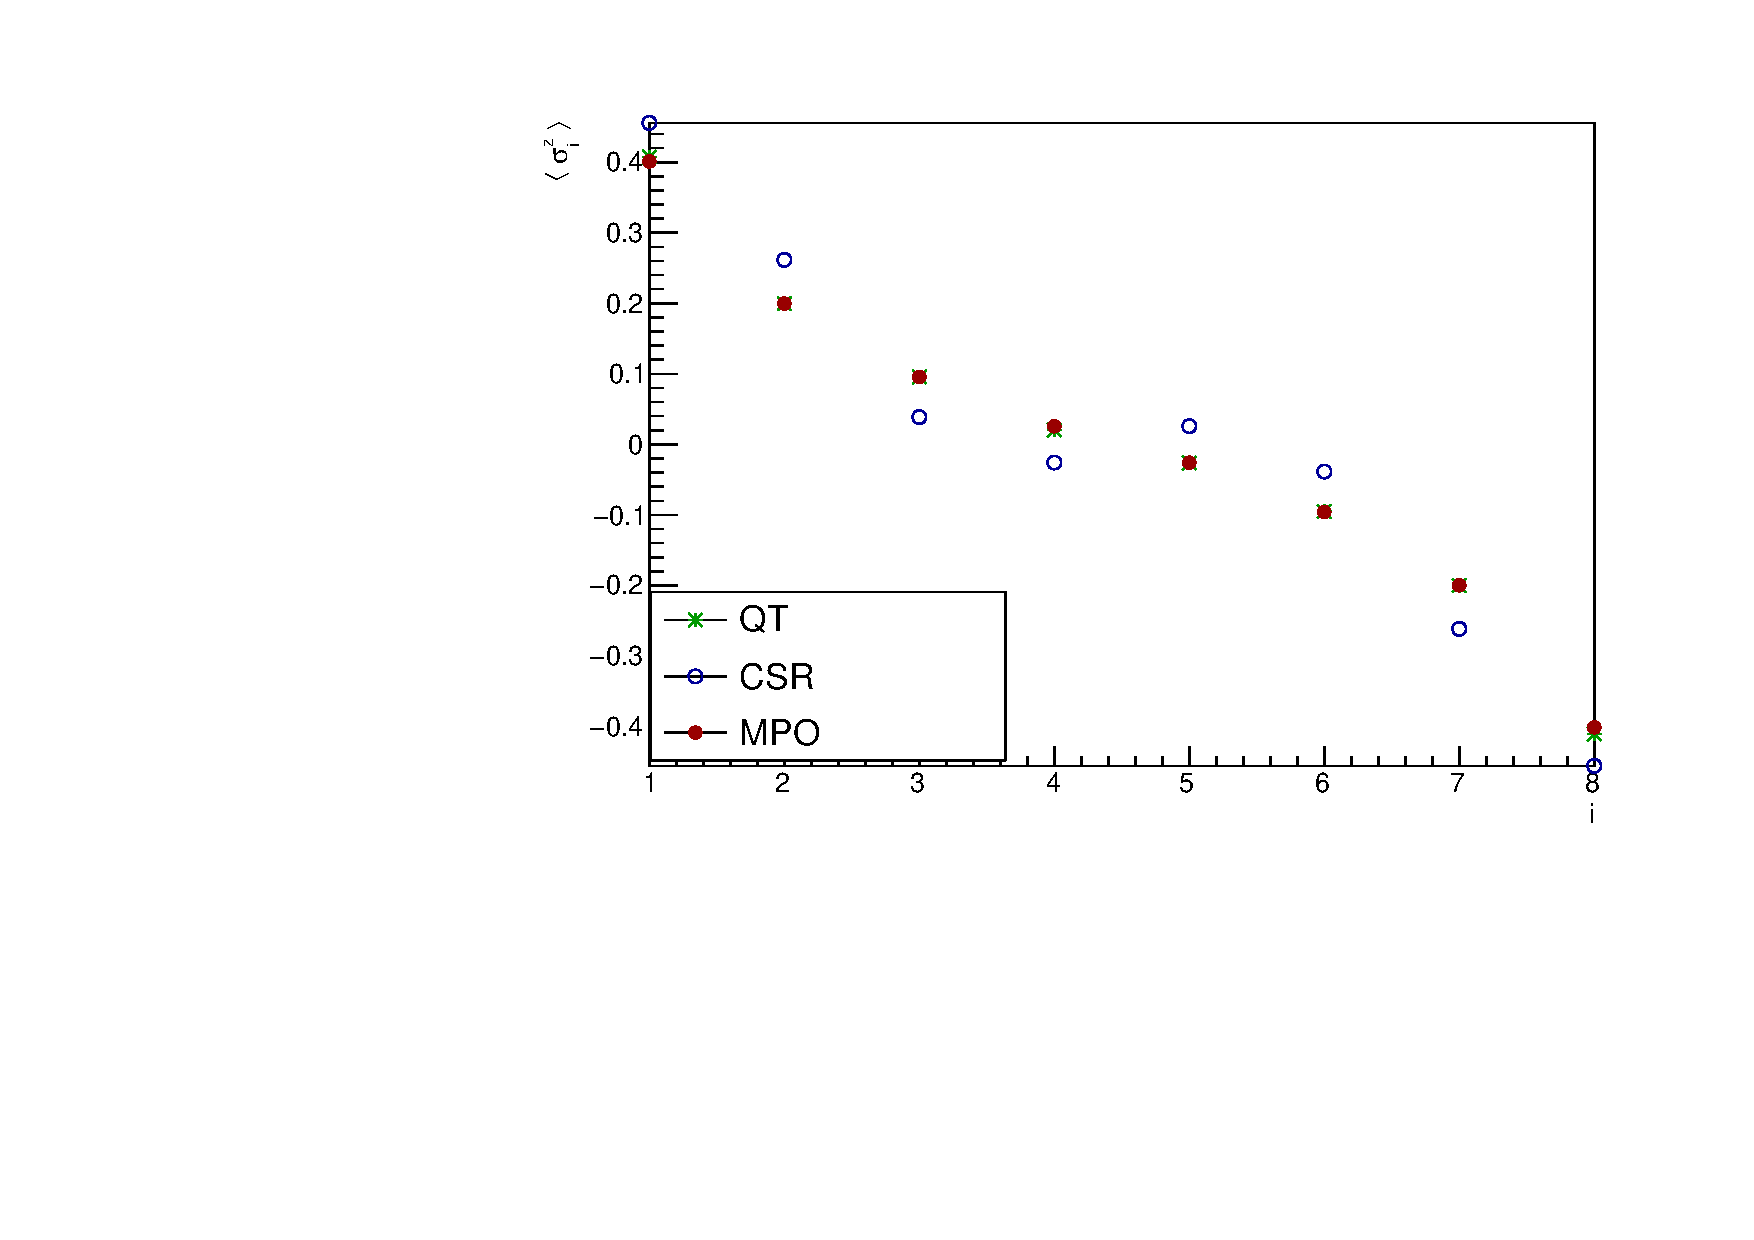
\includegraphics[scale=0.7]{Figures/8sites/LMComparison_8sJ1051.pdf}
    \captionsetup{width=1.\linewidth}
    \caption{Spin profile for a 8-sites chain characterized by $\gamma=1, J_x=1, J_y=1, J_z=1$; \\ \emph{i} stands for the site index.}
    \label{fig:8sites_LMcomparisonJz1}
\end{figure}

Now, it is interesting to investigate how the change of chain length modifies the magnetization profile. In fig.~\ref{fig:LM_comparisonVSsizeJz1Gamma1} it is shown the comparison between the magnetization profile of chains with different lengths. Two characteristics stand out: the first one is the fact that the peak values of $\langle\sigma^z\rangle$ in the ends of the chain are independent from the size of the system; this is true also for different values of $\gamma$: the peak values still remains the same for different lengths of the chain; the second one involves the fact that increasing the length of the chain, the spin profile gets flatter.

\begin{figure}[H]
    \centering
    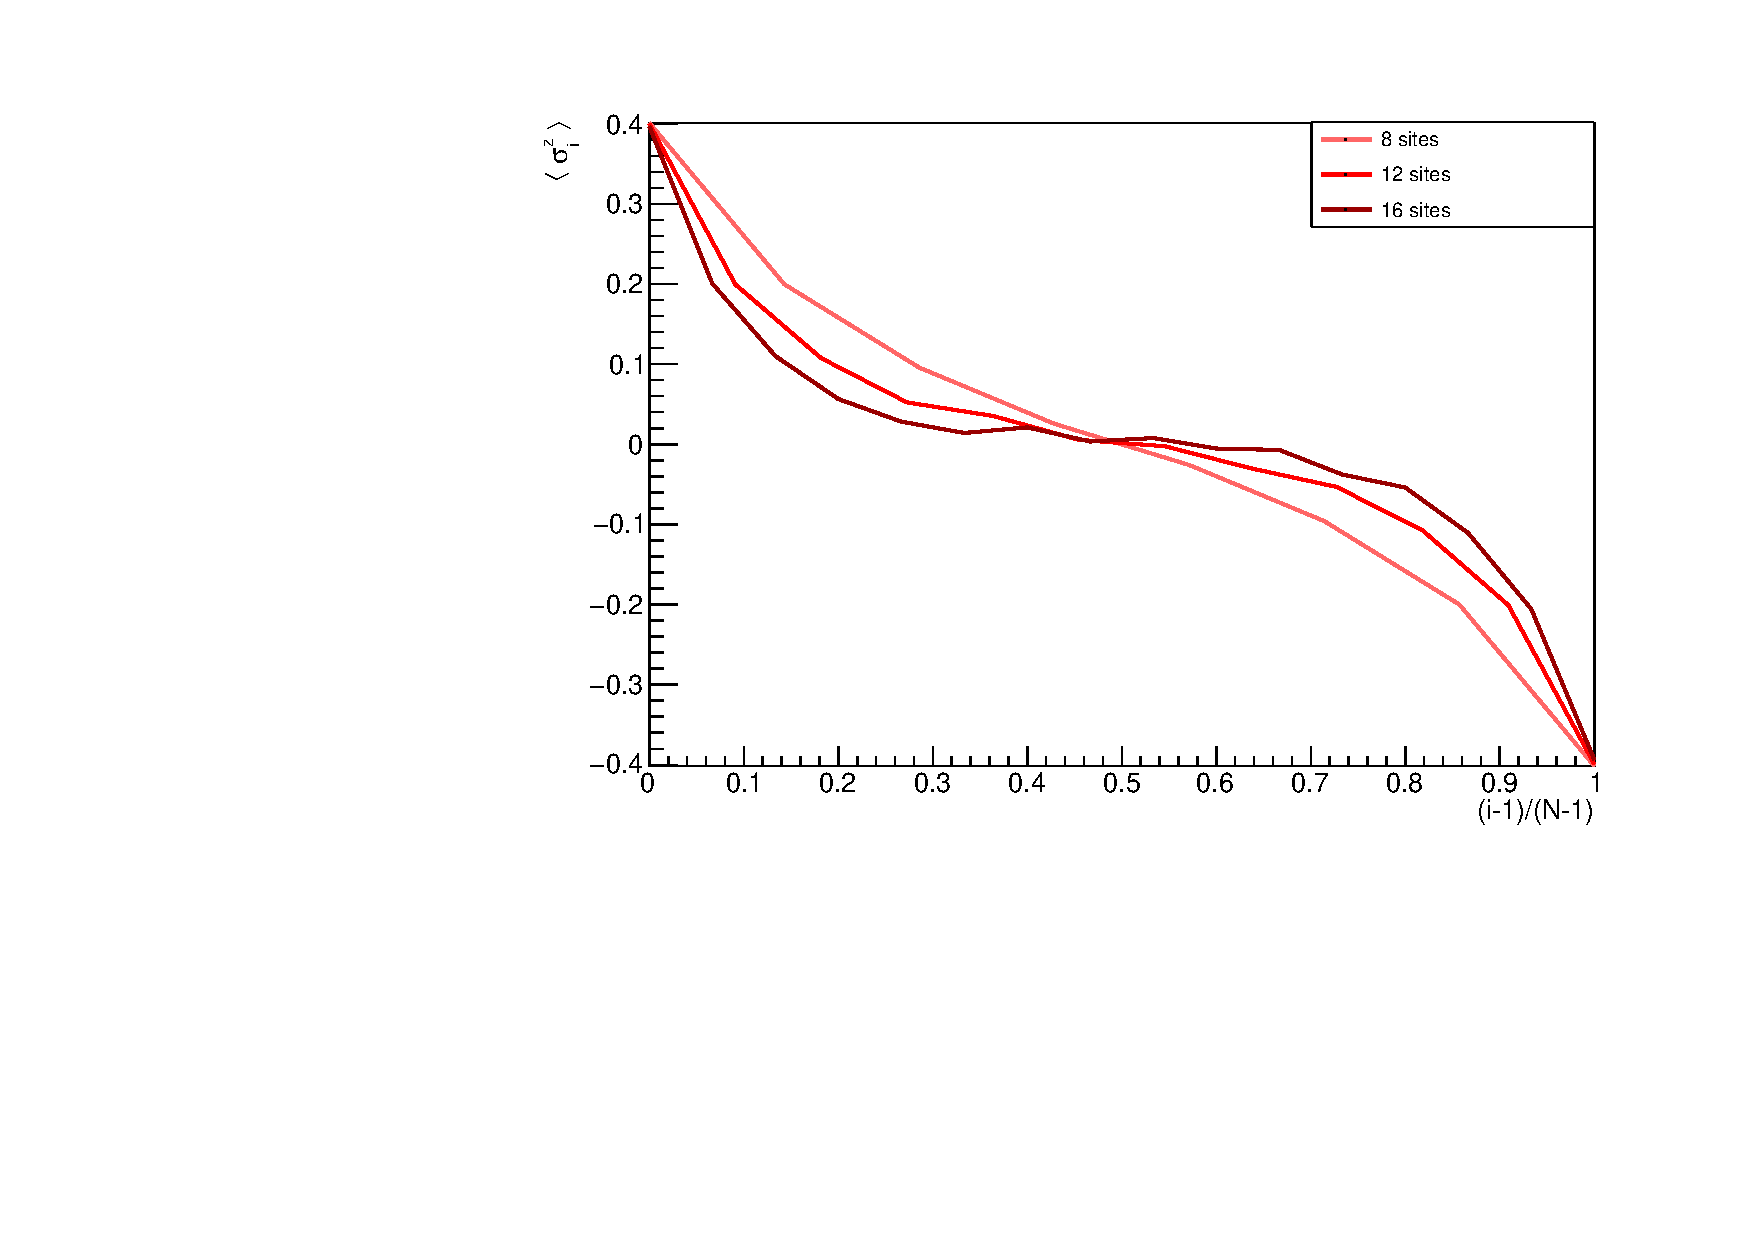
\includegraphics[scale=0.7]{Figures/NORM_LM_comparisonVSsize.pdf}
    \captionsetup{width=1.\linewidth}
    \caption{Spin profile for the model under study at $J_z = 1$ and $\gamma=1$. Data for different chain length are shown and they are obtained from MPO method.}
    \label{fig:LM_comparisonVSsizeJz1Gamma1}
\end{figure}

In order to analyze these properties in more detail, in the following figures we see how the behaviour of magnetization profile changes for different values of dissipation rate $\gamma$. 

First of all, it is convenient separate the curves for each size (8, 12 and 16 sites) in order to distinguish the profiles. The plots are shown in figures~\ref{fig:8sites_LMvsGamma},~\ref{fig:12sites_LMvsGamma},~\ref{fig:16sites_LMvsGamma}.

It is worth noting several aspects that arise from these plots. First of all, it seems clear that, while increasing $\gamma$, the ends of the chain become more and more polarized. This is true for every length of the chain because, as mentioned previously, the peak values are independent of the length of the chain.

The profile is not trivially linear, but changes while $\gamma$ changes. This trend becomes more and more evident as the length increases. Indeed, while $L$ grows, the plots show with increasing clearness the formation of a \emph{plateau} in which the magnetization is zero. Only near the edges it tends to boost, because of the driving effect of the dissipators.


\begin{figure}[H]
    \centering
    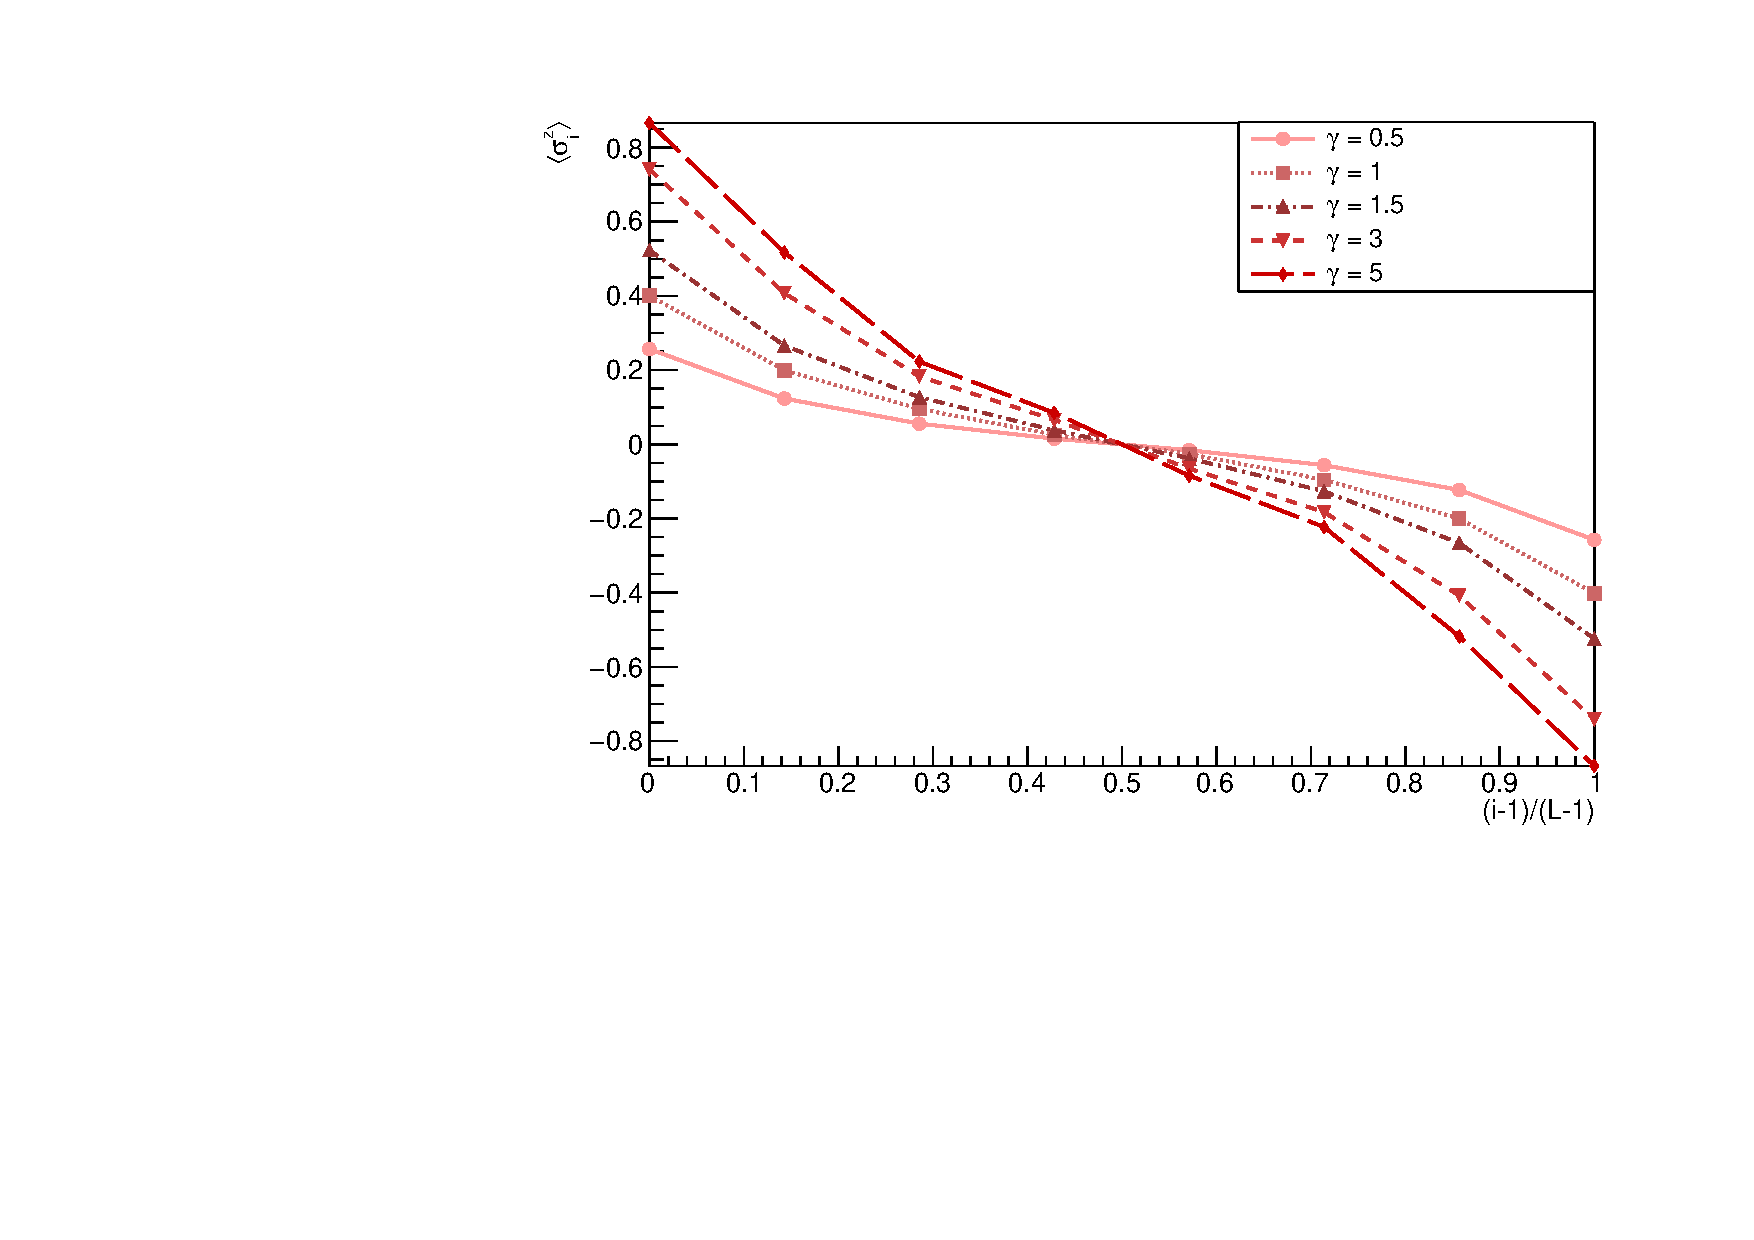
\includegraphics[scale=0.7]{Figures/8sites/8sites_LMvsGamma.pdf}
    \captionsetup{width=1.\linewidth}
    \caption{Spin profile for a 8-sites chain varying on dissipation rate $\gamma$. Data are obtained from MPO method.}
    \label{fig:8sites_LMvsGamma}
\end{figure}

\begin{figure}[H]
    \centering
    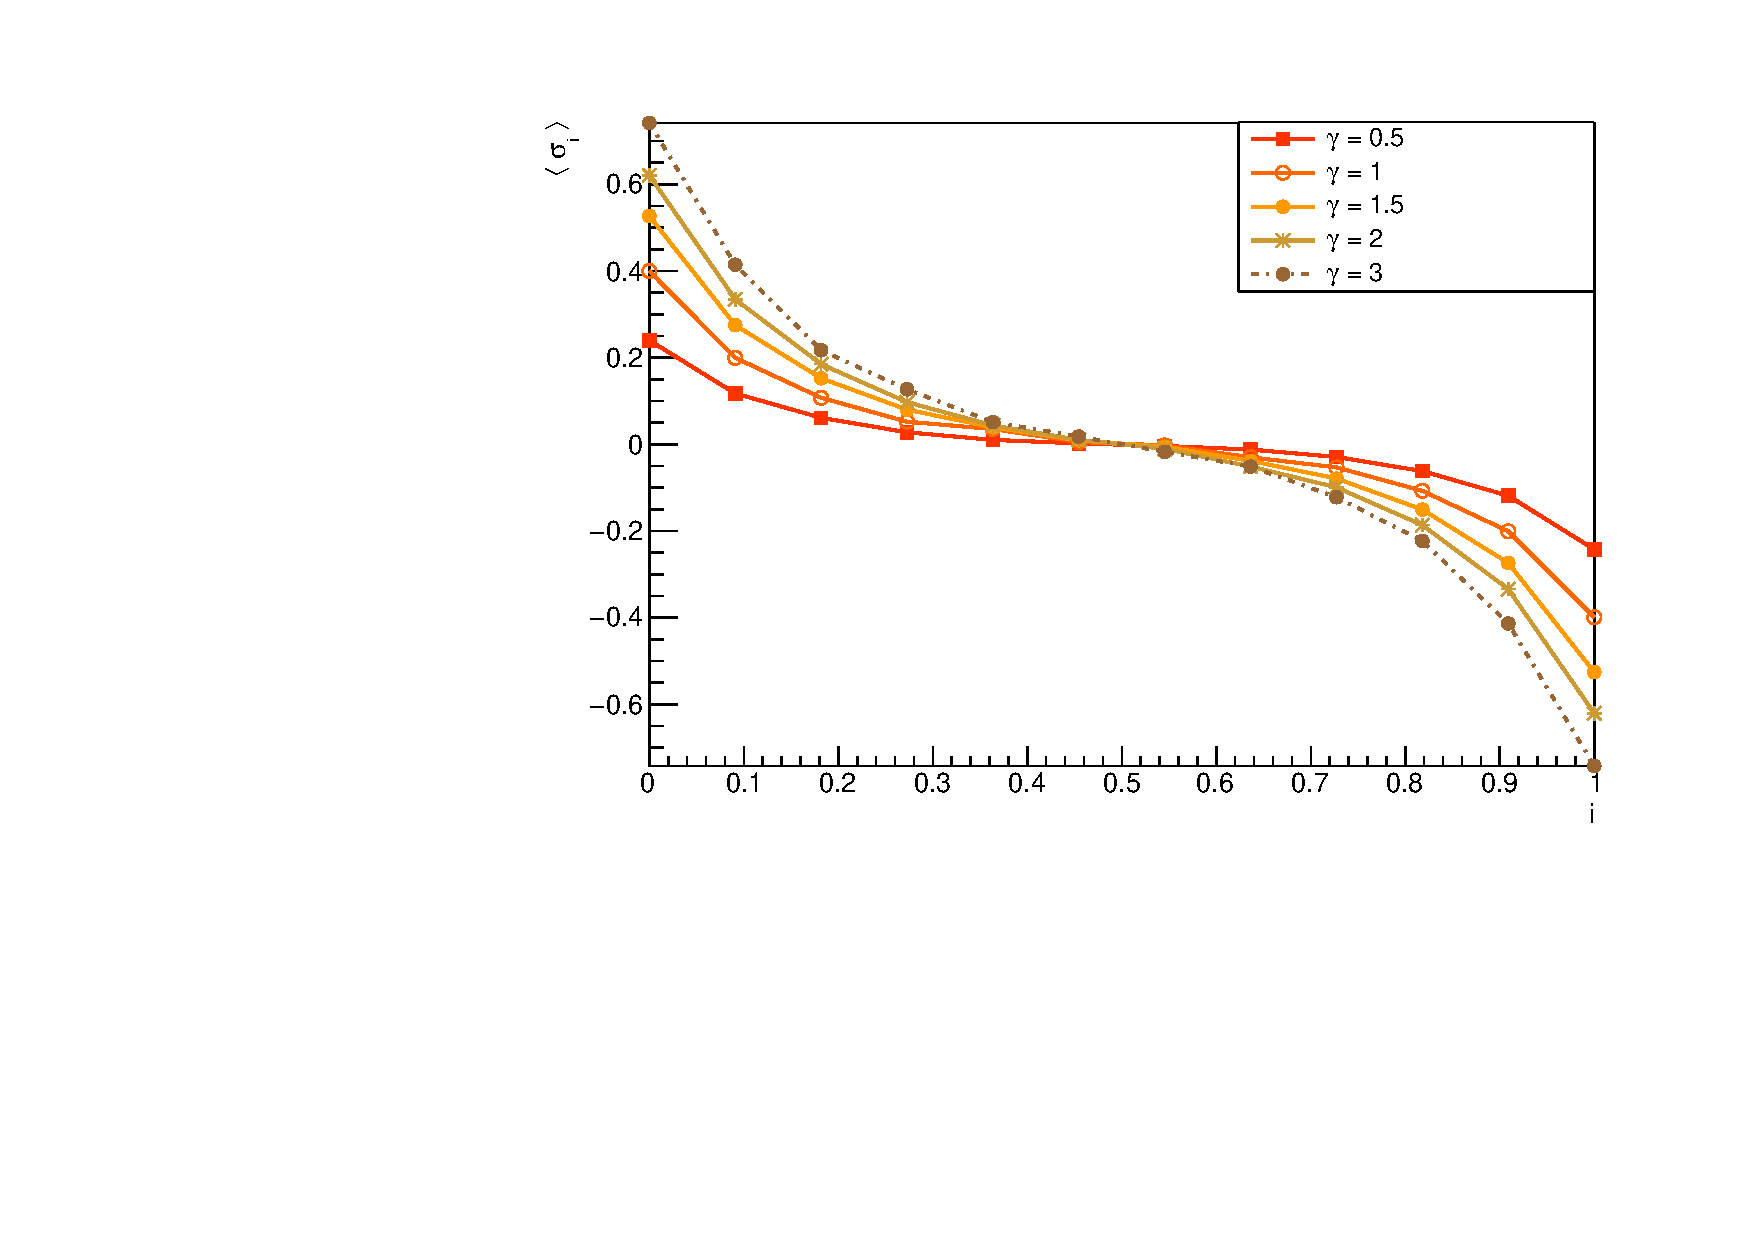
\includegraphics[scale=0.7]{Figures/12sites/12sites_LMvsGamma.pdf}
    \captionsetup{width=1.\linewidth}
    \caption{Spin profile for a 12-sites chain varying on dissipation rate $\gamma$. Data are obtained from MPO method.}
    \label{fig:12sites_LMvsGamma}
\end{figure}

\begin{figure}[H]
    \centering
    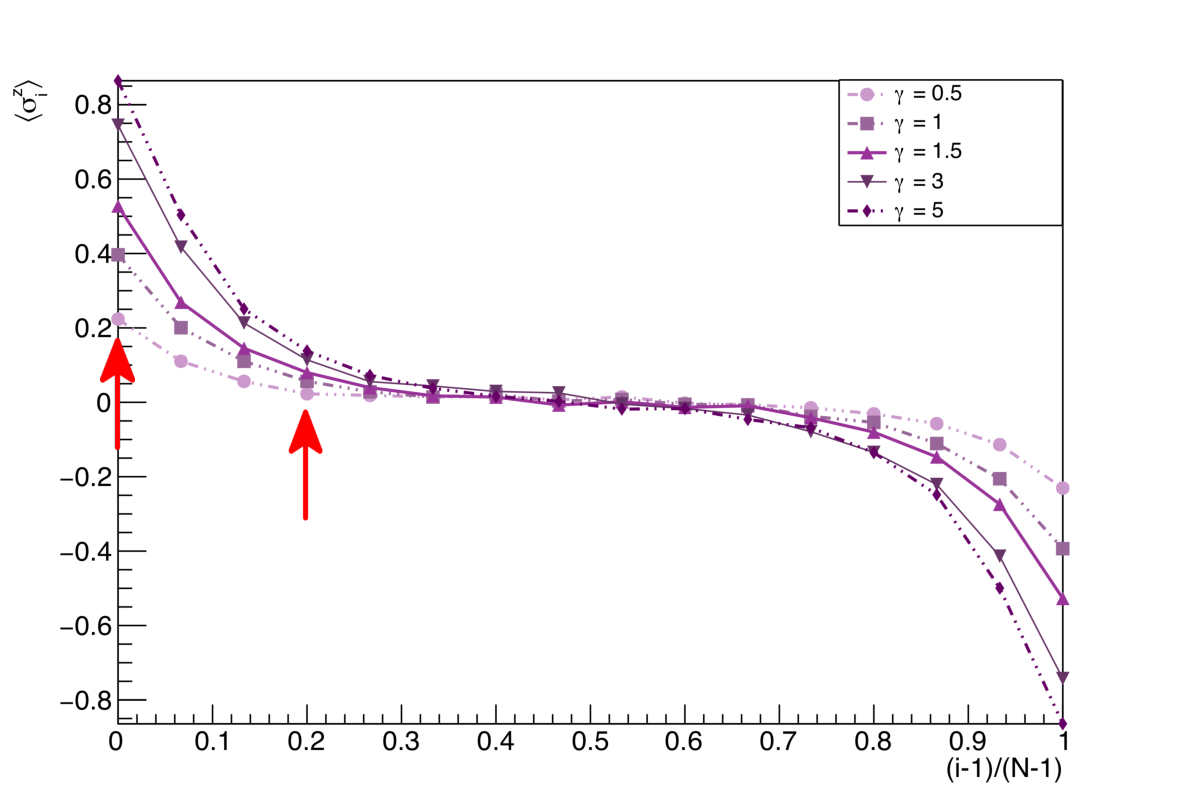
\includegraphics[scale=0.7]{Figures/16sites/16sites_LMvsGamma.pdf}
    \captionsetup{width=1.\linewidth}
    \caption{Spin profile for a 16-sites chain varying on dissipation rate $\gamma$. Data are obtained from MPO method.}
    \label{fig:16sites_LMvsGamma}
\end{figure}

As said previously, the peak value of $\langle\sigma^z\rangle$ varies with $\gamma$. In the fig.~\ref{fig:FIT_PeakLMvsGamma_J1051} it is presented the fit~\cite{root_cern} that shows an exponential behaviour. 

\begin{figure}[H]
    \centering
    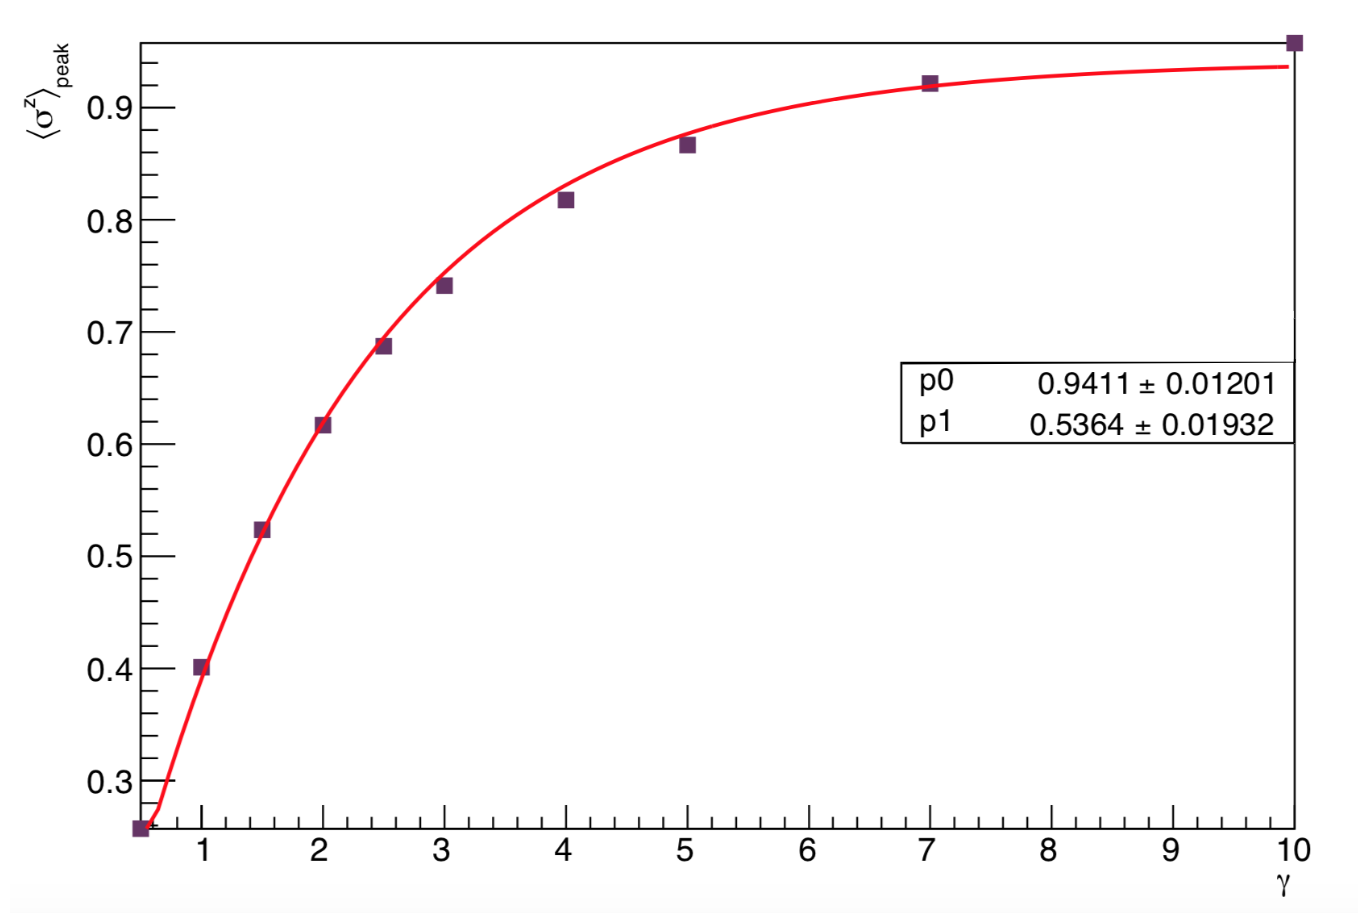
\includegraphics[scale=0.5]{Figures/FIT_PeakLMVsGamma.png}
    \captionsetup{width=1.\linewidth}
    \caption{The red line shows the fit $\langle\sigma^z\rangle_{max} = p_0(1-e^{-p_1\gamma})$.}
    \label{fig:FIT_PeakLMvsGamma_J1051}
\end{figure}

It is interesting noting that the same dependence is keep also by $\langle\sigma^z\rangle$ of spins lying in the $\frac{L}{4}$-th site, as shown in fig.~\ref{fig:FIT_16sites_4thSiteVSgamma} (the same trend is confirmed in the case of 8 and 12 sites, shown in \textcolor{red}{appendix?}).

\begin{figure}[H]
    \centering
    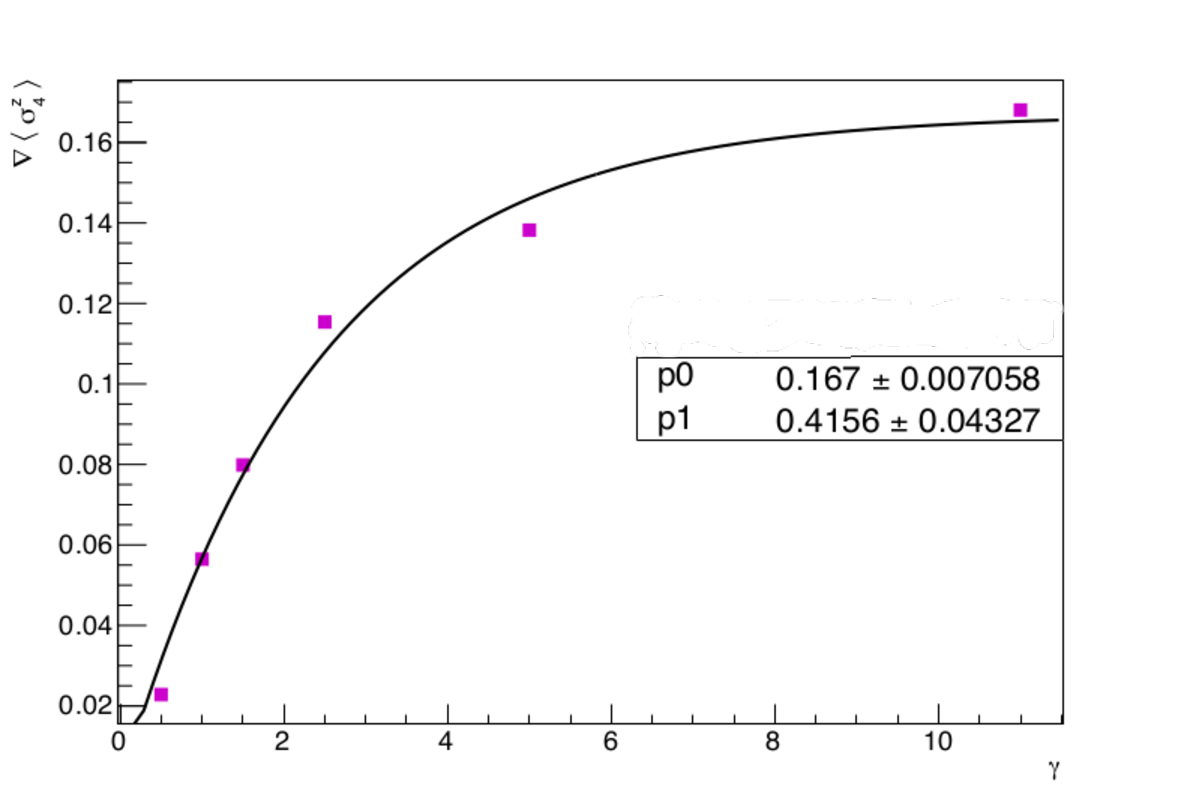
\includegraphics[scale=0.7]{Figures/16sites/FIT_16sites_4thSiteVSgamma.pdf}
    \captionsetup{width=1.\linewidth}
    \caption{16 sites, the black line shows the fit $\langle\sigma^z_{4th}\rangle(\gamma) = p_0(1-e^{-p_1\gamma})$. 
    \\textcolor{red}{Error in the label of y-axis.}}
    \label{fig:FIT_16sites_4thSiteVSgamma}
\end{figure}

These two plots displayed in fig.~\ref{fig:FIT_PeakLMvsGamma_J1051} and in fig.~\ref{fig:FIT_16sites_4thSiteVSgamma} show that for large values of $\gamma$, i.e. for more and more important driving, $\langle\sigma^z\rangle$ tends asymptotically to a maximum value.

%In the following, we study the gradient of magnetization for the middle sites in the 8-sites chain. In fig.~\ref{fig:FIT_8sites_gradLM23VSgamma}, \ref{fig:FIT_12sites_gradLM34VSgamma}, \ref{fig:FIT_16sites_gradLM45VSgamma} the gradient of magnetization between the spin lying in the $\frac{N}{4}$-th site and the neighbouring site. The profile here shown, seems to confirm the fits in fig.\ref{fig:FIT8sites_LM_2ndSiteVSgamma}, \ref{fig:FIT12sites_3rdSiteVSgamma}, \ref{fig:FIT_16sites_4thSiteVSgamma}.

%\begin{figure}[H]
    %\centering
    %\includegraphics[scale=0.7]{Figures/8sites/FIT_8sites_gradLMcente%rVSgamma.pdf}
    %\caption{8 sites, the red line shows the fit \\$\nabla %\langle\sigma^z\rangle_{center}(\gamma) = %-p_0+p_1\exp{(-p_2\gamma)}$.}
    %\label{fig:FIT_8sites_gradLMcenterVSgamma}
%\end{figure}

%\begin{figure}[H]
    %\centering
    %\includegraphics[scale=0.7]{Figures/8sites/FIT_8sites_gradLM23VSg%amma.pdf}
    %\caption{8 sites, the red line shows the fit \\$\nabla %\langle\sigma^z\rangle_{2-3}(\gamma) = %-p_0+p_1\exp{(-p_2\gamma)}$.}
    %\label{fig:FIT_8sites_gradLM23VSgamma}
%\end{figure}

%\begin{figure}[H]
    %\centering
    %\includegraphics[scale=0.7]{Figures/12sites/FIT_12sites_gradLM34V%Sgamma.pdf}
    %\caption{12 sites, the orange line shows the fit \\$\nabla %\langle\sigma^z\rangle_{3-4}(\gamma) = %-p_0+p_1\exp{(-p_2\gamma)}$.}
    %\label{fig:FIT_12sites_gradLM34VSgamma}
%\end{figure}

%\begin{figure}[H]
    %\centering
    %\includegraphics[scale=0.7]{Figures/16sites/FIT_16sites_gradLM45V%Sgamma.pdf}
    %\captionsetup{width=1.\linewidth}
    %\caption{16 sites, the black line shows the fit $\nabla %\langle\sigma^z\rangle_{4-5}(\gamma) = %-p_0+p_1\exp{(-p_2\gamma)}$.}
    %\label{fig:FIT_16sites_gradLM45VSgamma}
%\end{figure}

%In the following, a comparison between the profiles of the chain of different size.

%\begin{figure}[H]
    %\centering
    %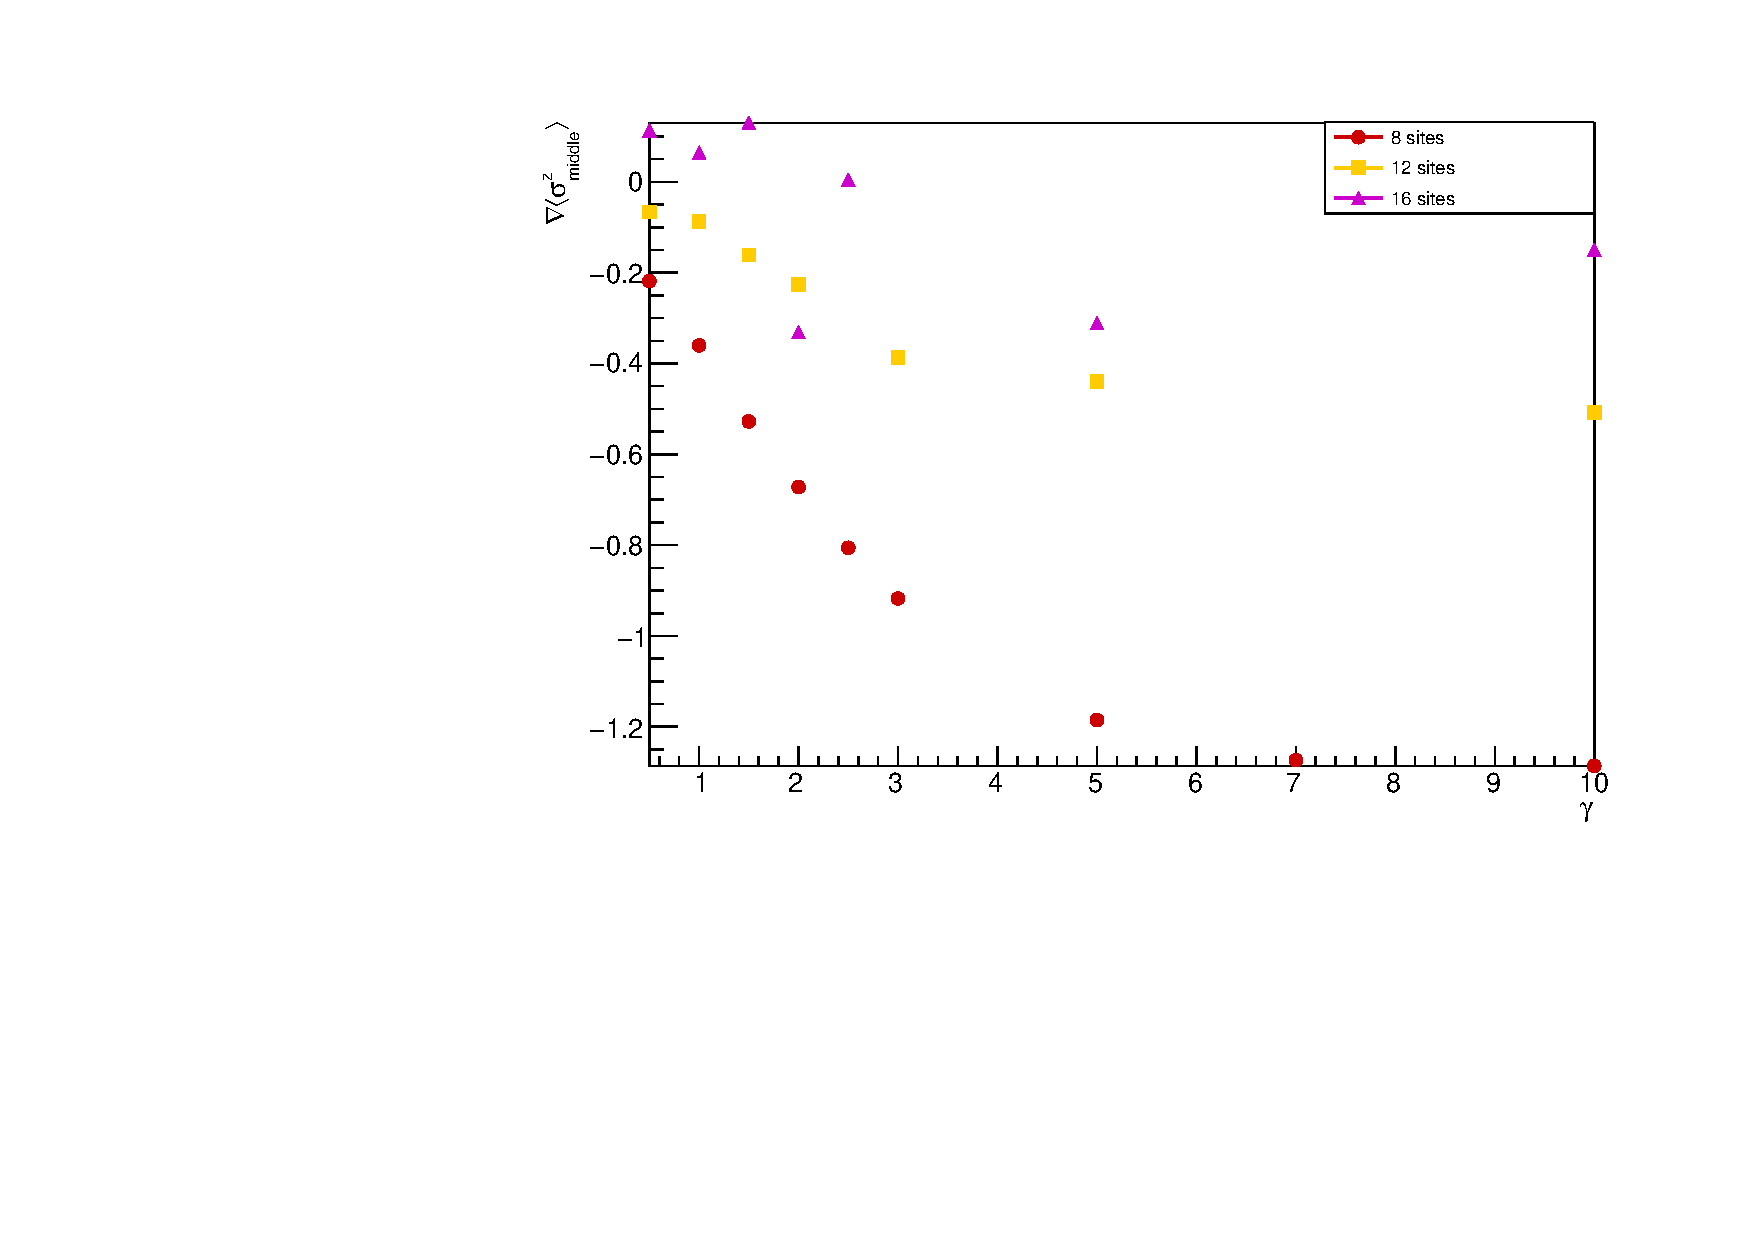
\includegraphics[scale=0.7]{Figures/gradLMvsGammavsSize.pdf}
    %\caption{Gradient of magnetization for the middle sites in 8, 12, %16-sites chain versus $\gamma$.}
    %\label{fig:gradLMvsGammavsSize}
%\end{figure}

%\begin{figure}[H]
    %\centering
    %\includegraphics[scale=0.7]{Figures/gradLMvsGammavsSize_firstQuar%terChain.pdf}
    %\caption{Gradient of magnetization for the sites lying in the %$\frac{N}{4}$-th site in 8, 12, 16-sites chain versus $\gamma$.}
    %\label{fig:gradLMvsGammavsSize_firstQuarterChain}
%\end{figure}


%%%%%%%%%%%%%%%%%%%%%%%%%%%%%%%%%%%%%%%%%%%%%%%%%%%%%%%%%%%%%%%%%%%%%%%%%%%%%%%%%%%%%%%%%%%%%%%%%%%%%%%%%%%%%%%%%%%%%%%%%%%%%%%%%%%%%%%%%%%%%%%%%%%%%%%%%%%%%%%%%%%%%%%%%%%%%%%%%%%%%%%%%%%%%%%%%%%%%%%%%%%%%%%%%%%%%%%%%%%%%%%%%%%%%%%%%%%%%%%%%%%%%%%%%%%%%%%%%%%%%
\section{Two-Points Correlation Functions}
Another observable of interest is certainly the steady-state two-point correlation function, defined as follows:
\begin{equation}
    C(i, j) = \langle \sigma^z_i \sigma^z_j \rangle - \langle \sigma^z_i \rangle \langle \sigma^z_j \rangle,
\end{equation}
where $\langle \sigma^z_i \sigma^z_j \rangle = \Tr(\sigma^z_i \sigma^z_j \rho_{s})$ and $\langle \sigma^z_i \rangle = \Tr(\sigma^z_i \rho_{s})$, being $\rho_{s}$ the steady-state density matrix.

In particular, the two-point correlation function will be studied considering the system symmetry, using the so-called \emph{bulk} correlation function; that is, starting from the middle sites of the chain, the correlation function will be calculated between equidistant sites from the center of the chain. 

%First of all, as done in the last section, a comparison of the data obtained from MPO and QT method is shown; in particular, the spin-spin correlation function in relation to the first site $C(1, j)$ is displayed. In the following,

%\begin{figure}[H]
    %\centering
    %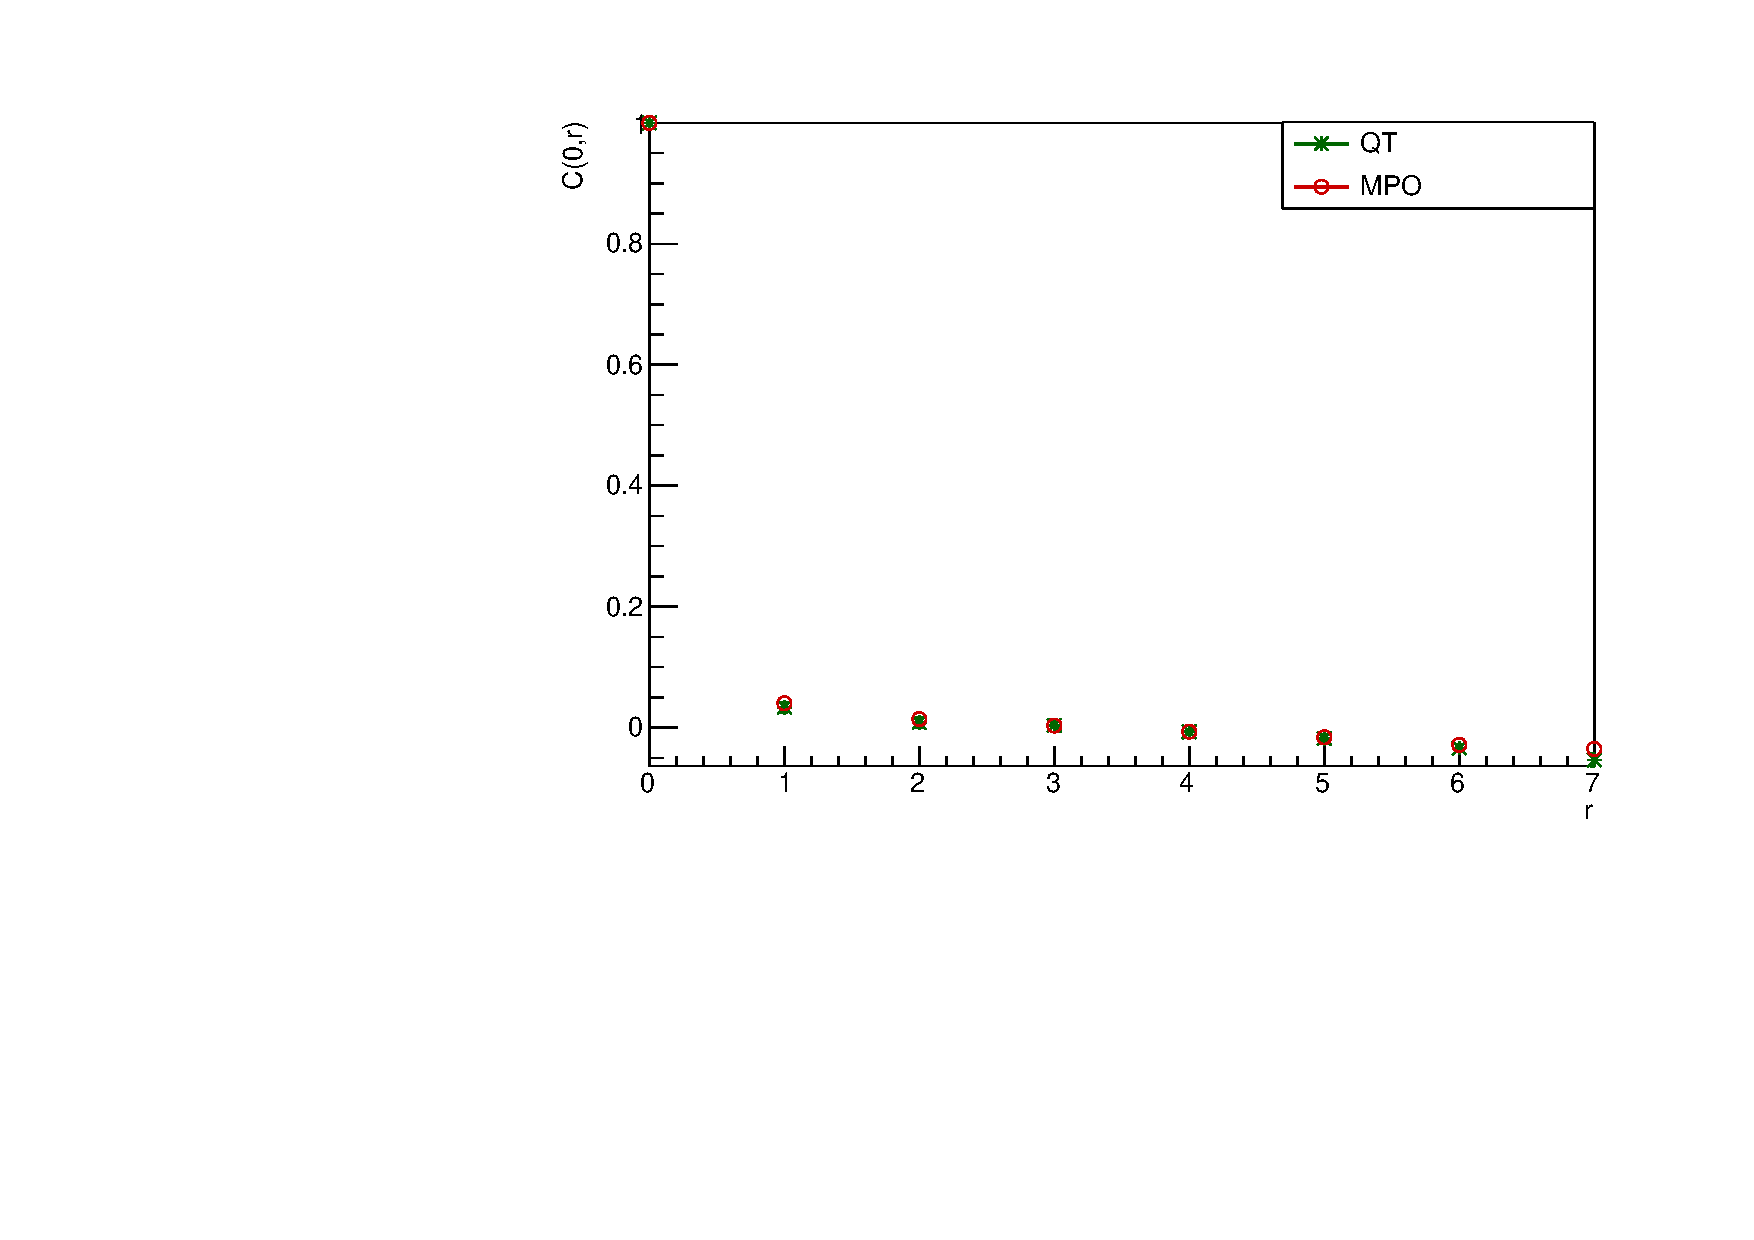
\includegraphics[scale=0.7]{Figures/8sites/CorrFunc1_8s_J10505.pdf}
    %\caption{Correlation function with respect to the spin positioned in the first %site of the chain, characterized by $\gamma~=~1, J_x=1, J_y=0.5, J_z=0.5$; %\emph{i} stands for the site index.}
    %\label{fig:my_label}
%\end{figure}

%\begin{figure}[H]
    %\centering
    %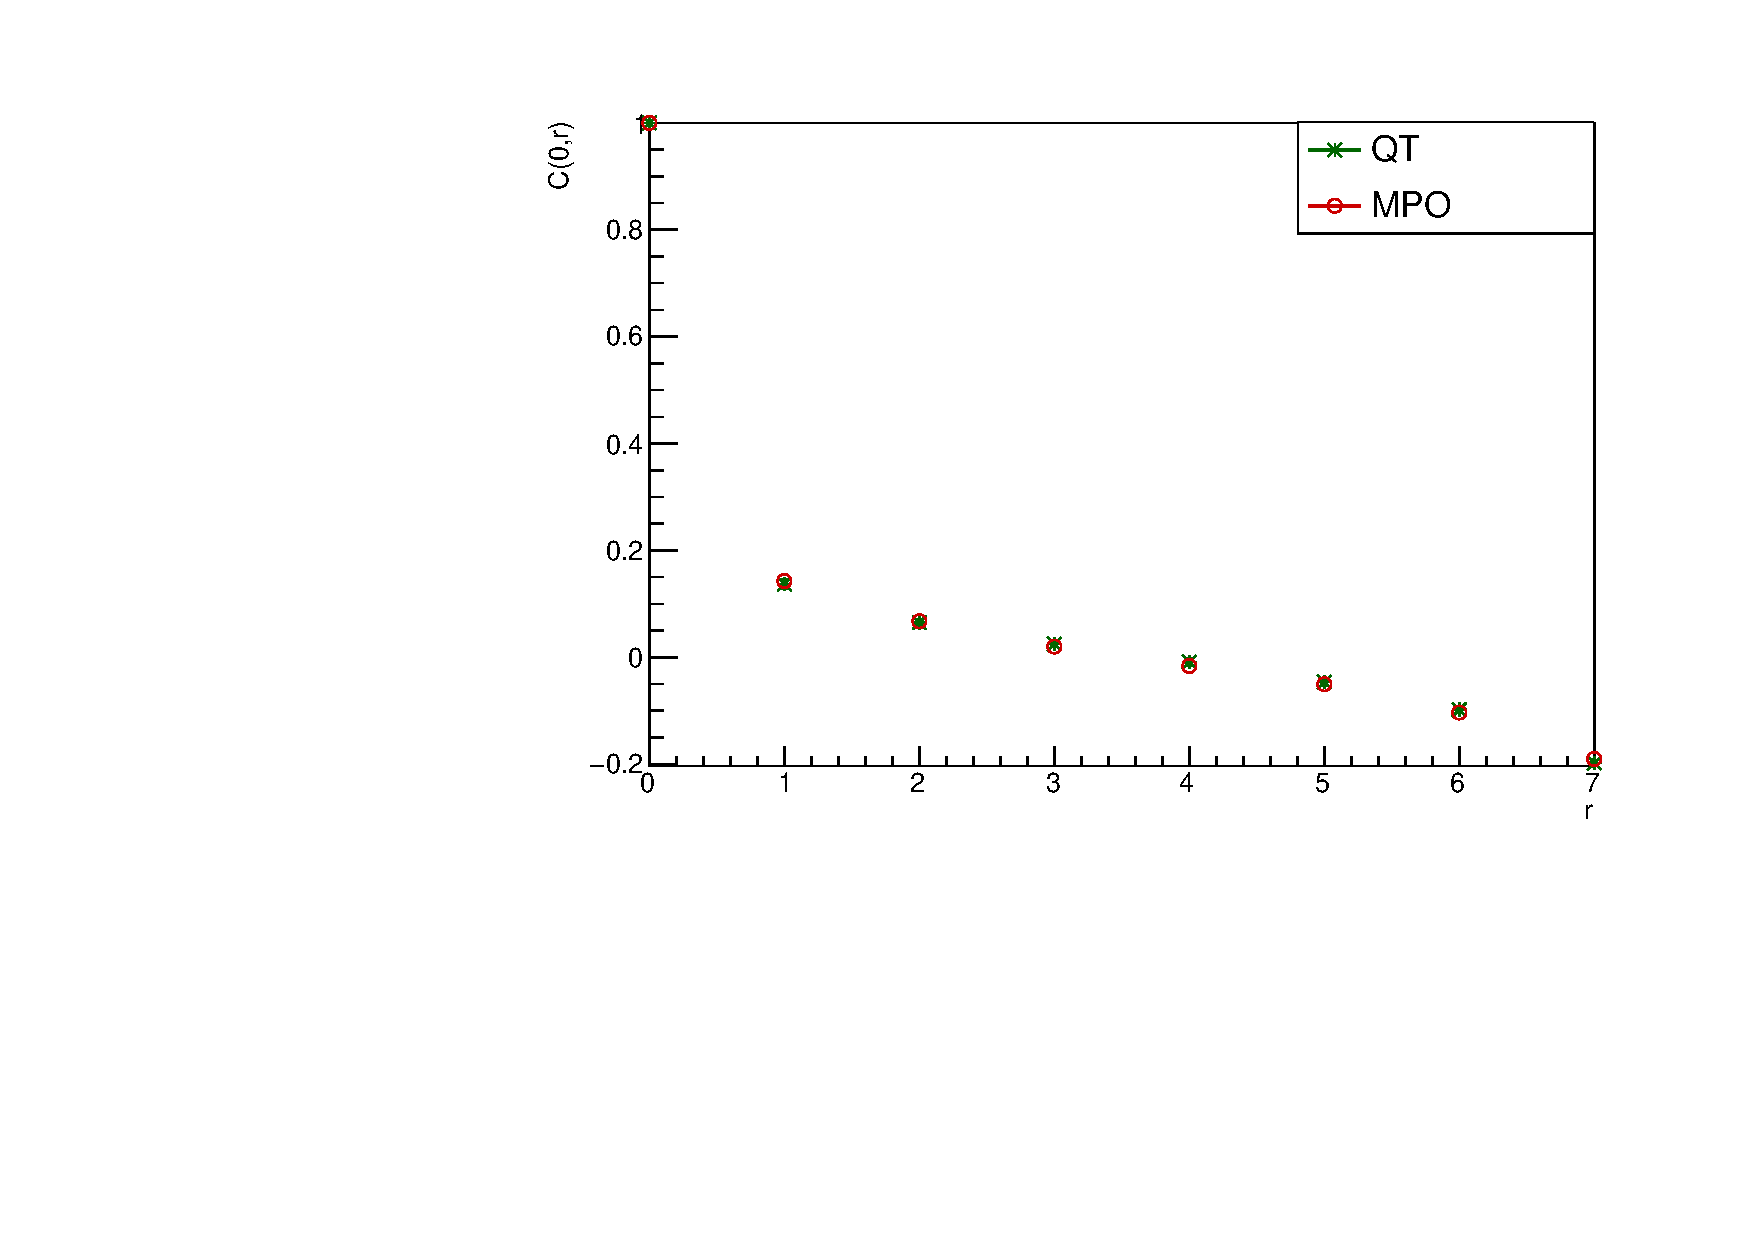
\includegraphics[scale=0.7]{Figures/8sites/CorrFunc1_8s_J1051.pdf}
    %\caption{Correlation function with respect to the spin positioned in the first %site of the chain, characterized by $\gamma~=~1, J_x=1, J_y=0.5, J_z=1$; %\emph{i} stands for the site index.}
    %\label{fig:my_label}
%\end{figure}

%\begin{figure}[H]
    %\centering
    %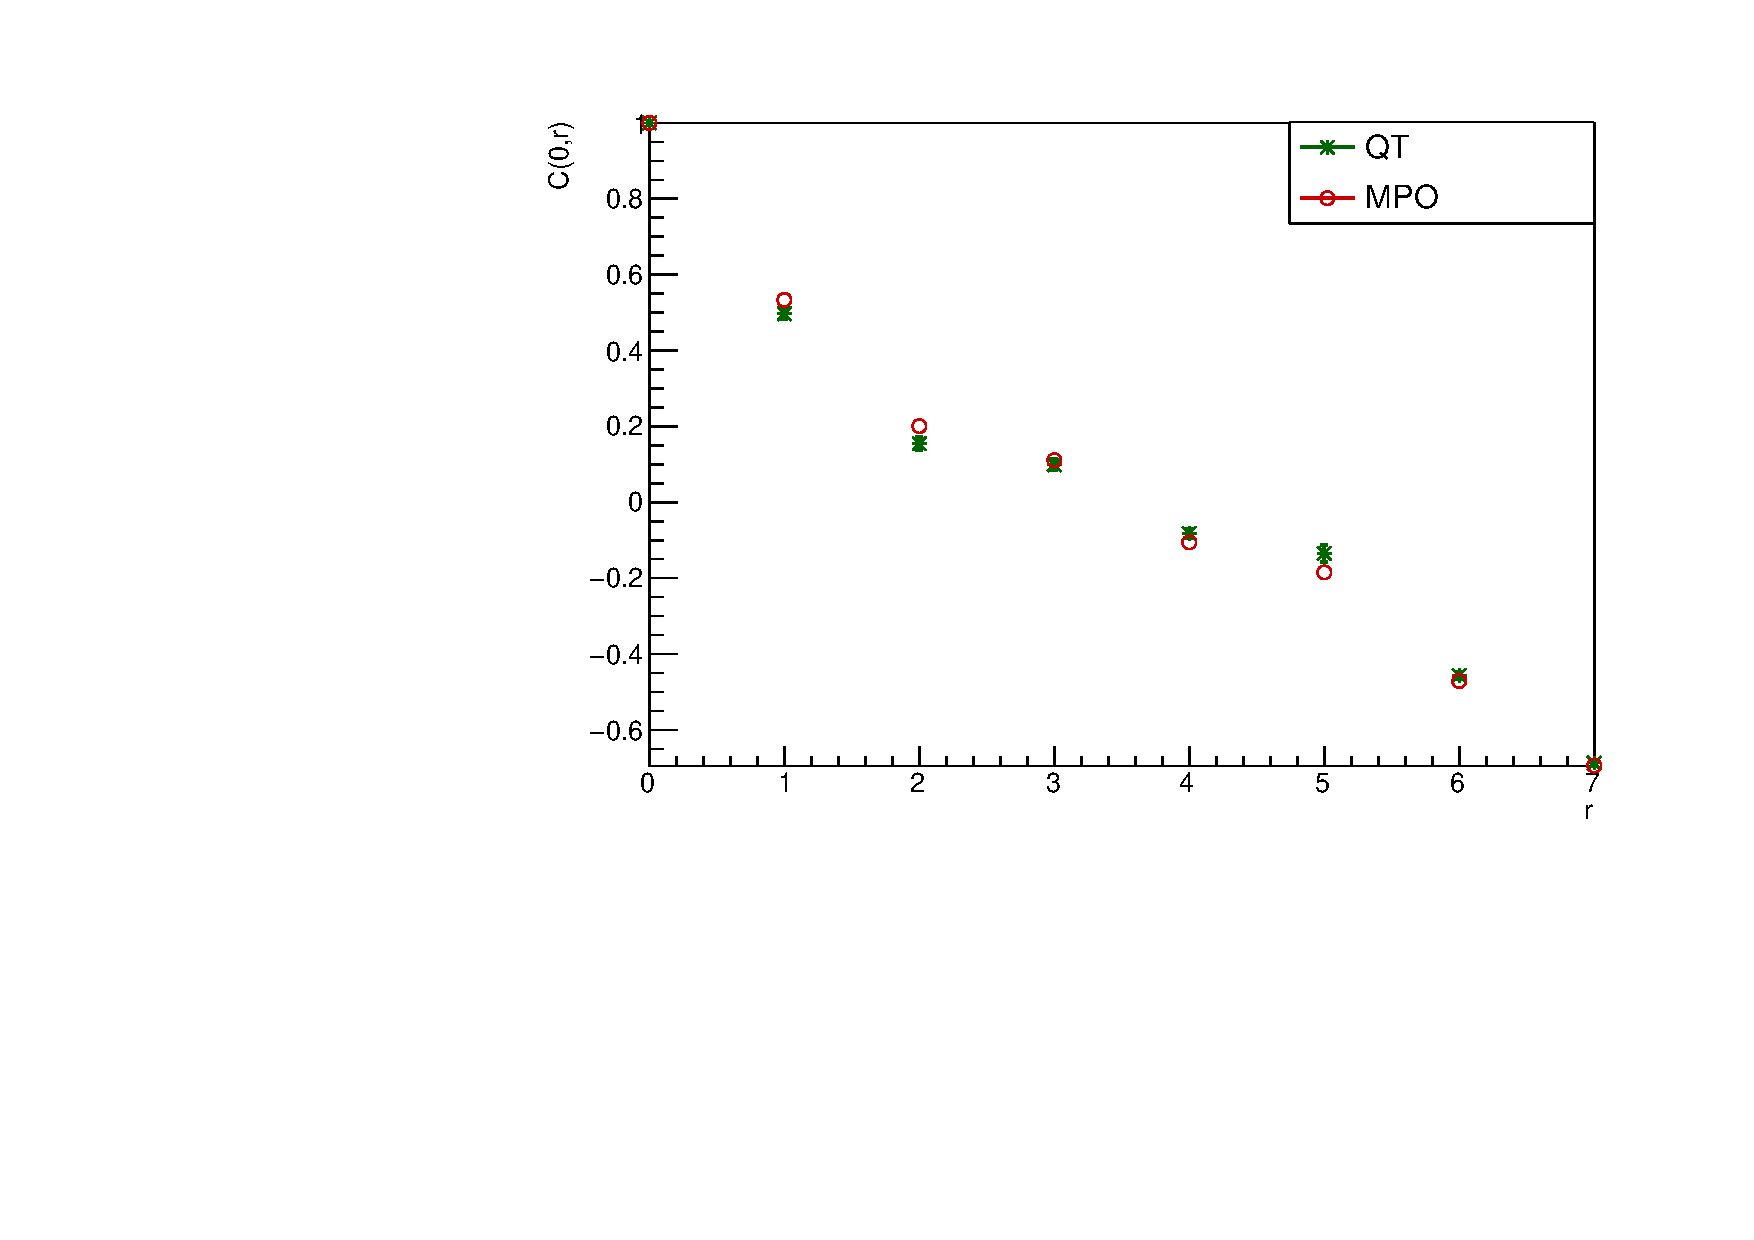
\includegraphics[scale=0.7]{Figures/8sites/CorrFunc1_8s_J10515.pdf}
    %\caption{Correlation function with respect to the spin positioned in the first %site of the chain, characterized by $\gamma~=~1, J_x=1, J_y=0.5, J_z=1.5$; %\emph{i} stands for the site index.}
    %\label{fig:my_label}
%\end{figure}

%The same is done for the bulk correlation function, calculated as explained previously.

%\begin{figure}[H]
    %\centering
    %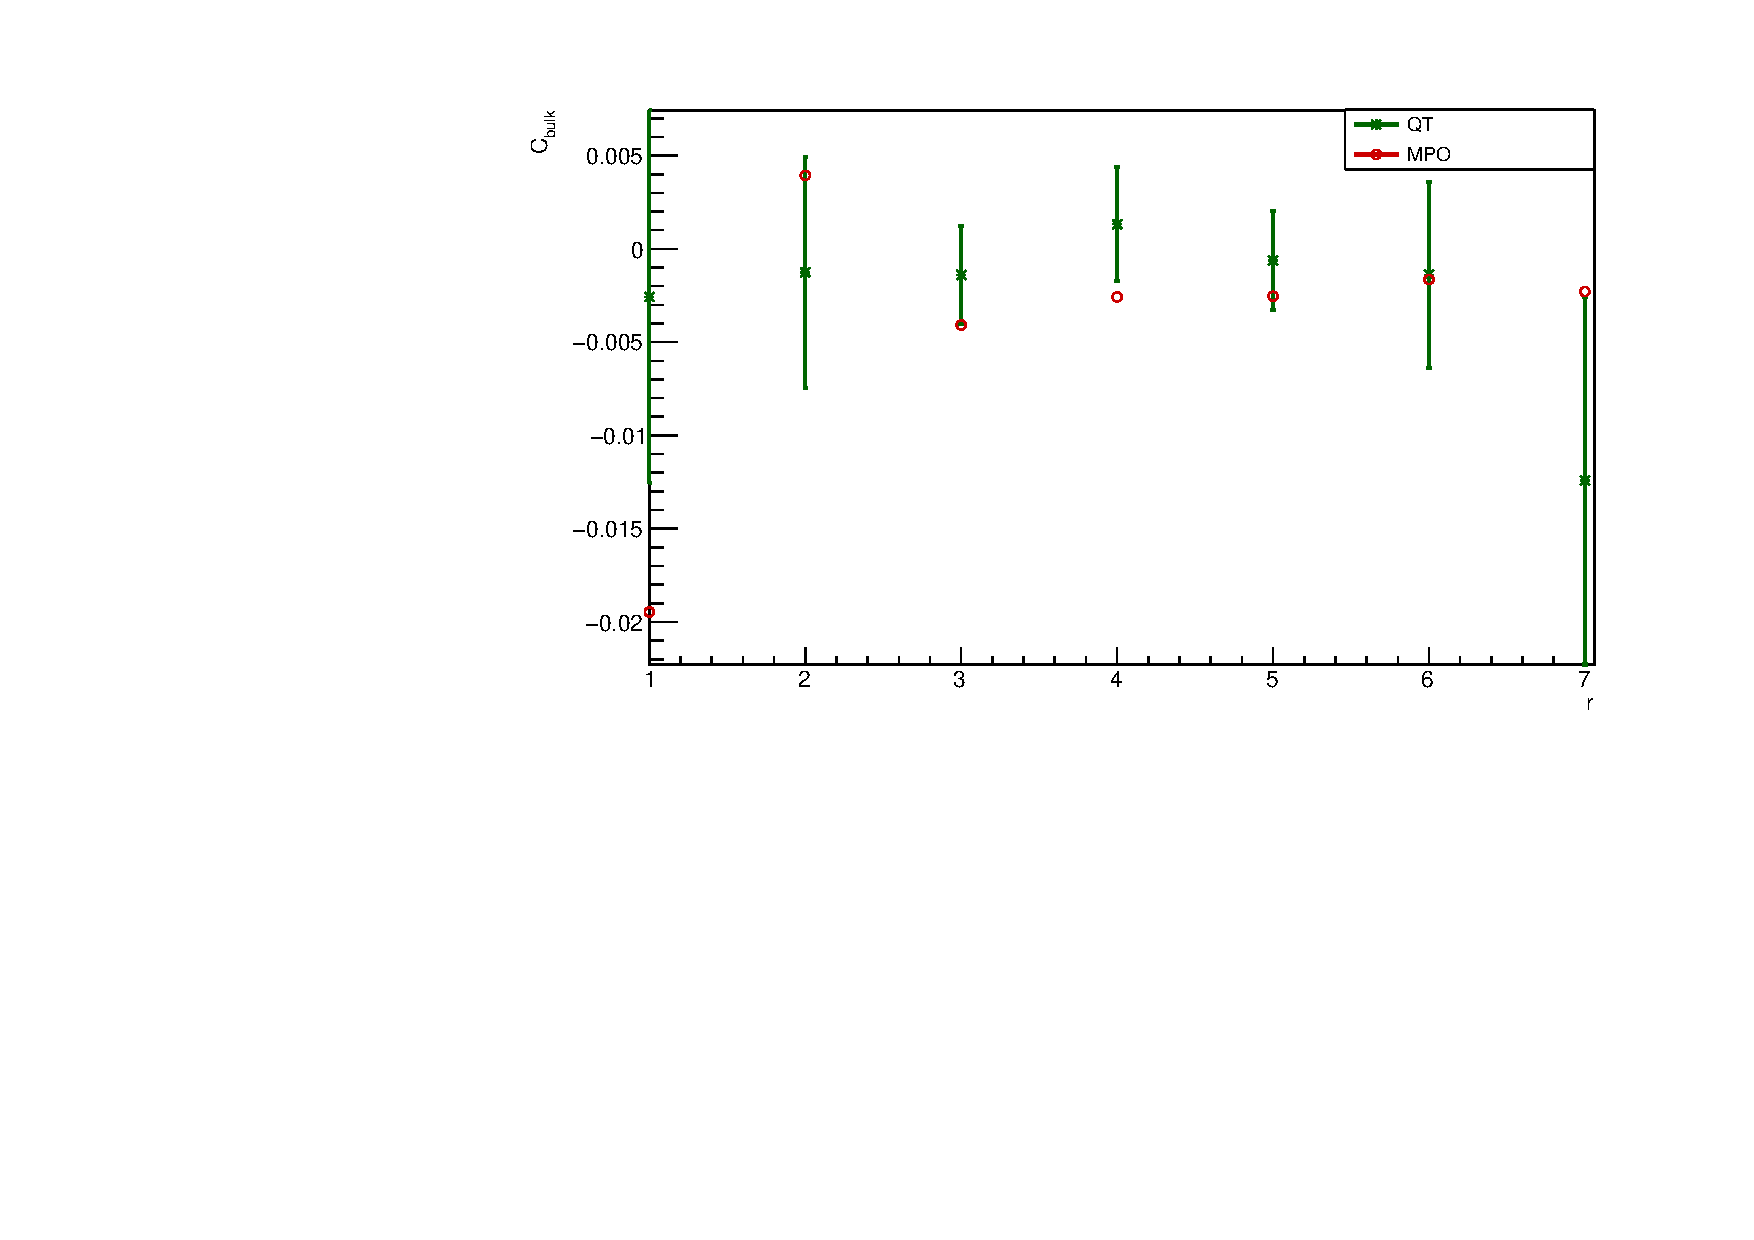
\includegraphics[scale=0.7]{Figures/8sites/CorrFuncBulkCONN_8sJ10505.pdf}
    %\caption{Bulk correlation function for a 8-sites chain characterized by %$\gamma~=~1, J_x=1, J_y=0.5, J_z=0.5$.}
    %\label{fig:my_label}
%\end{figure}

%\begin{figure}[H]
    %\centering
    %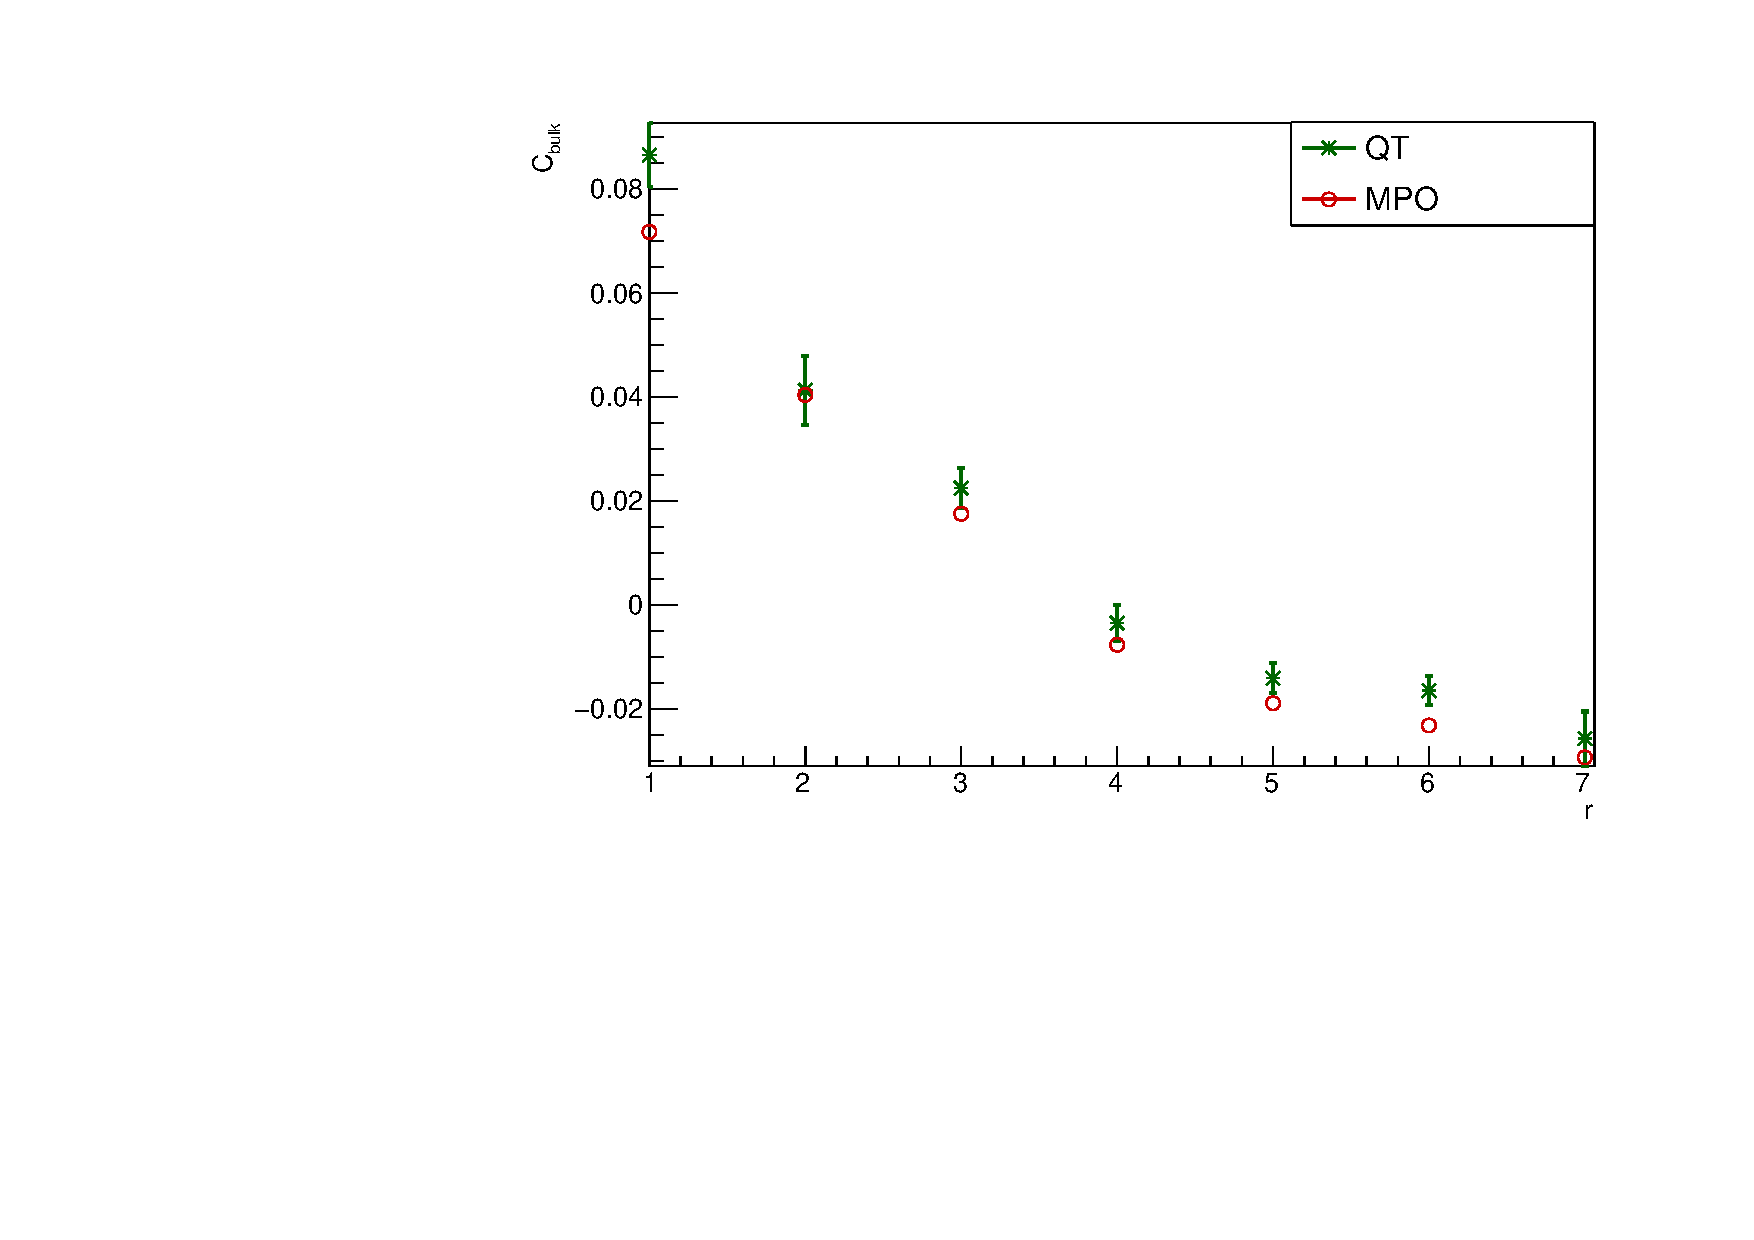
\includegraphics[scale=0.7]{Figures/8sites/CorrFuncBulkCONN_8sJ1051.pdf}
    %\caption{Bulk correlation function for a 8-sites chain characterized by %$\gamma~=~1, J_x=1, J_y=0.5, J_z=1$.}
    %\label{fig:my_label}
%\end{figure}

%\begin{figure}[H]
    %\centering
    %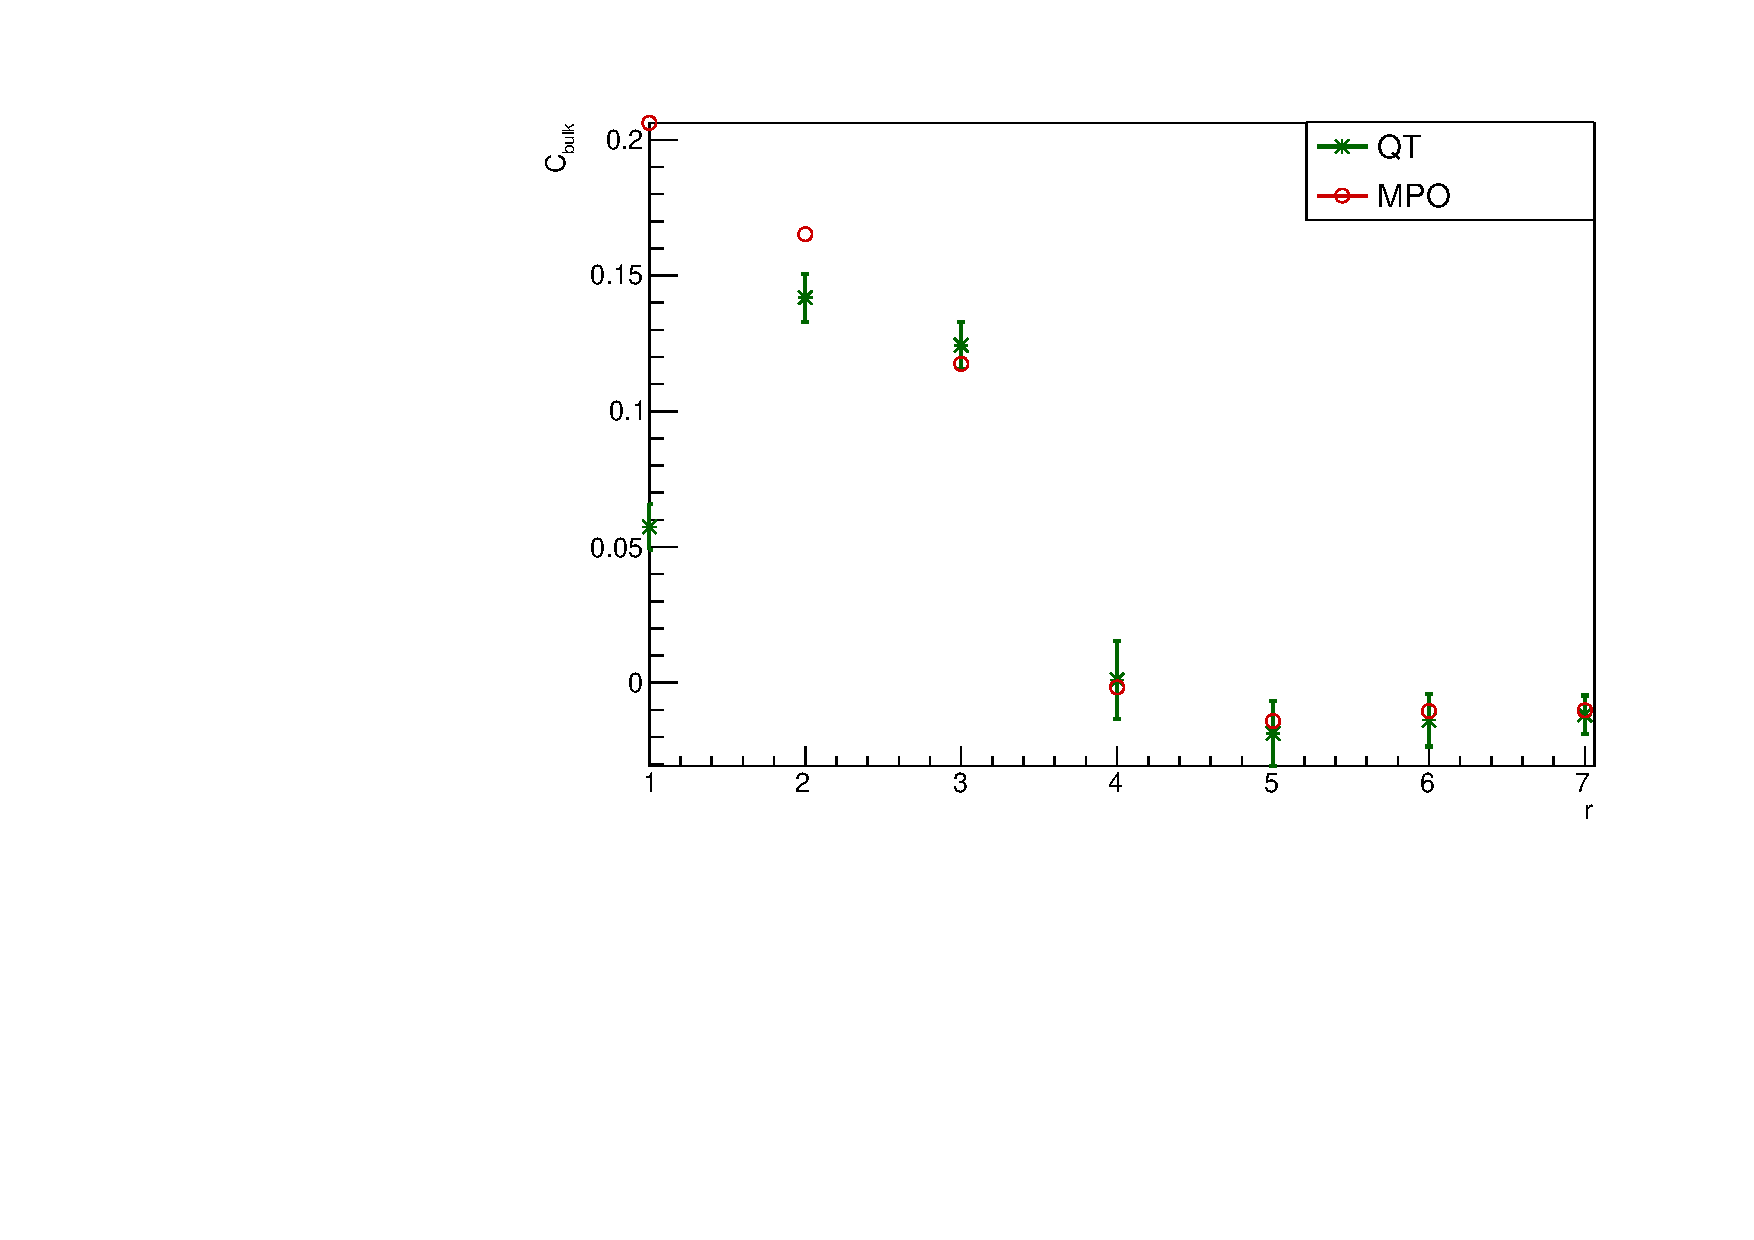
\includegraphics[scale=0.7]{Figures/8sites/CorrFuncBulkCONN_8sJ10515.pdf}
    %\caption{Bulk correlation function for a 8-sites chain characterized by %$\gamma~=~1, J_x=1, J_y=0.5, J_z=1.5$.}
    %\label{fig:my_label}
%\end{figure}

In the fig.~\ref{fig:8sites_CBulkConnVSgamma}, \ref{fig:12sites_CFBulkCONNVSgamma}, \ref{fig:16sites_CFBulkCONNVSgamma} the bulk correlation function for several values of $\gamma$ is shown, for 8, 12 and 16 sites spin chain respectively. An interesting aspect that is quite clear in these plots, involves the finite-size effect; while the size of the chain grows, the exponential profile of the correlation function become more clear. Indeed, only starting from size of 12 sites the exponential profile starts to stand out. 

\begin{figure}[H]
    \centering
    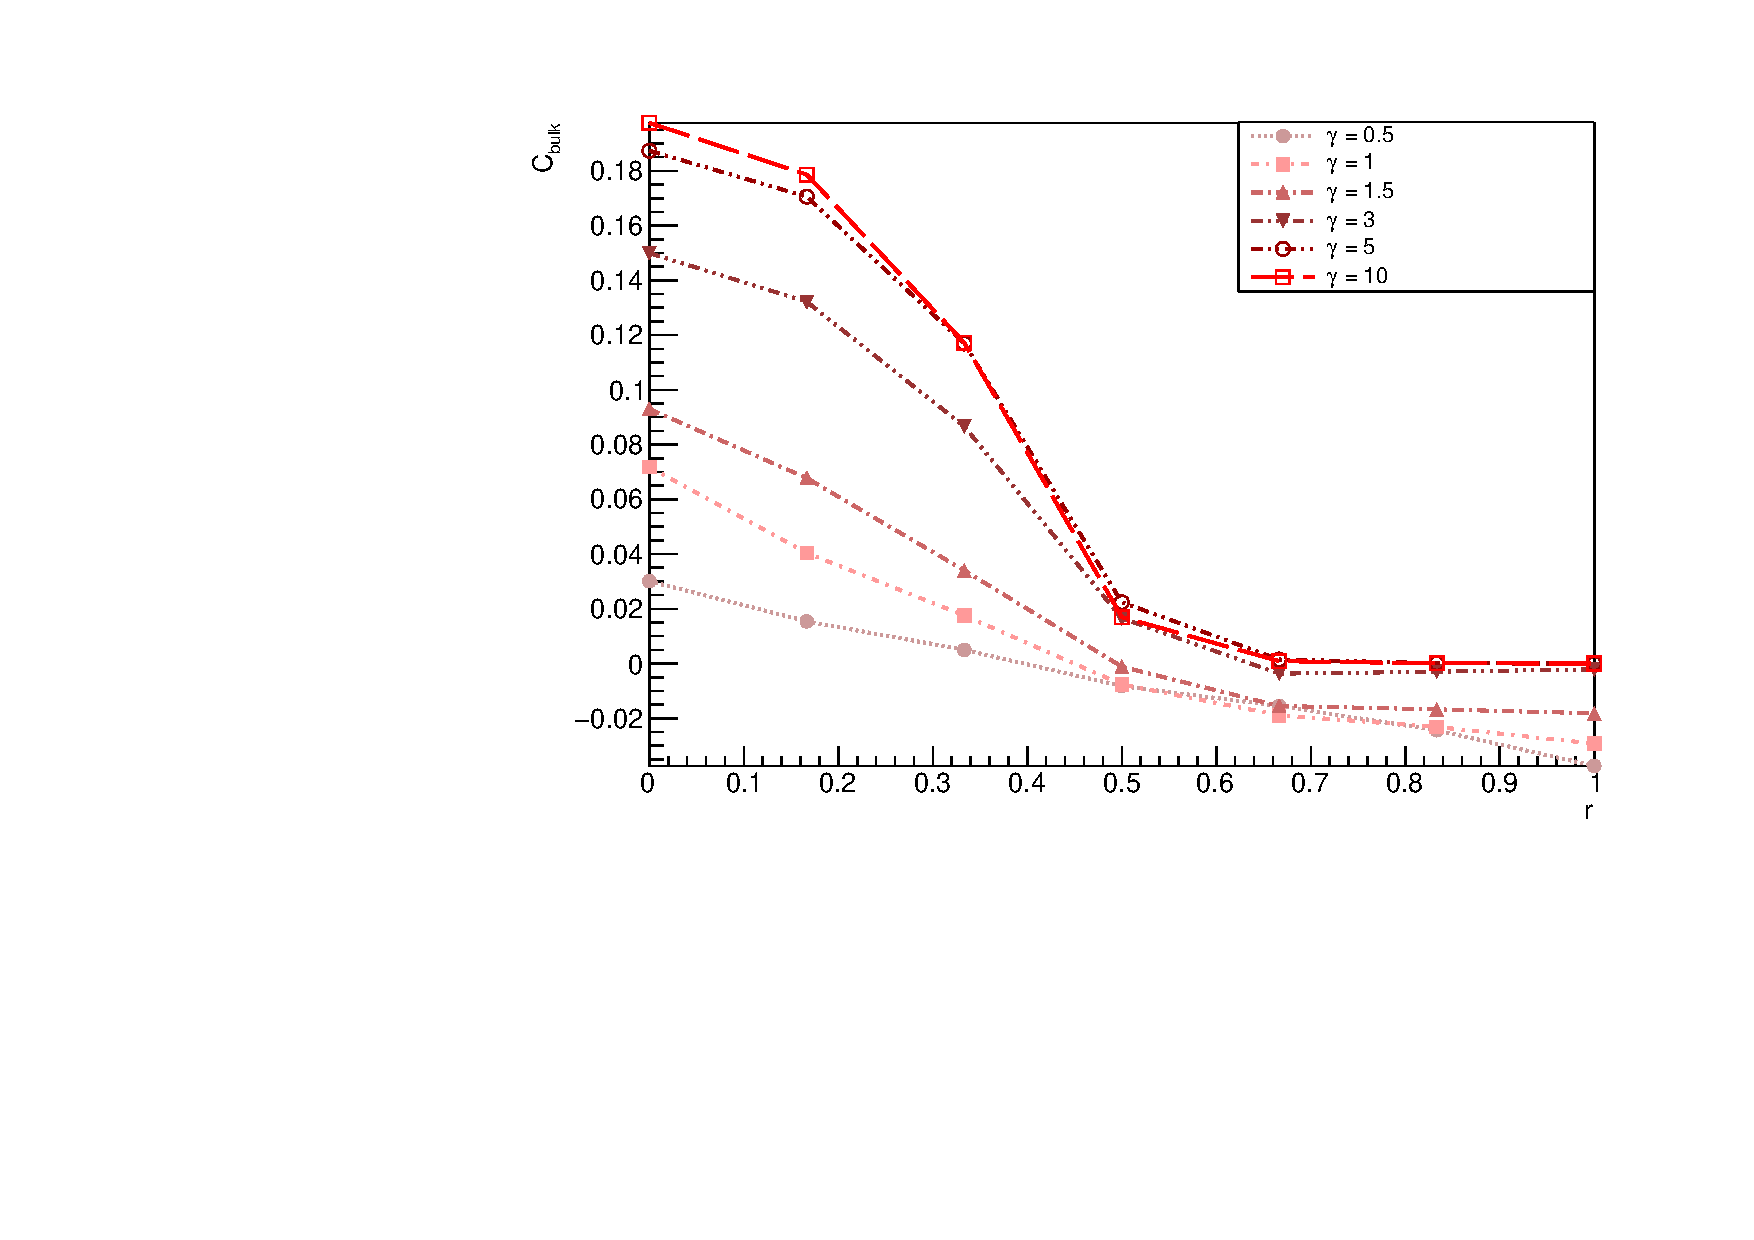
\includegraphics[scale=0.7]{Figures/8sites_CBulkConnVSgamma.pdf}
    \captionsetup{width=1.\linewidth}
    \caption{Bulk correlation function for a 8-sites spin chain. Data are obtained from MPO method.}
    \label{fig:8sites_CBulkConnVSgamma}
\end{figure}

\begin{figure}[H]
    \centering
    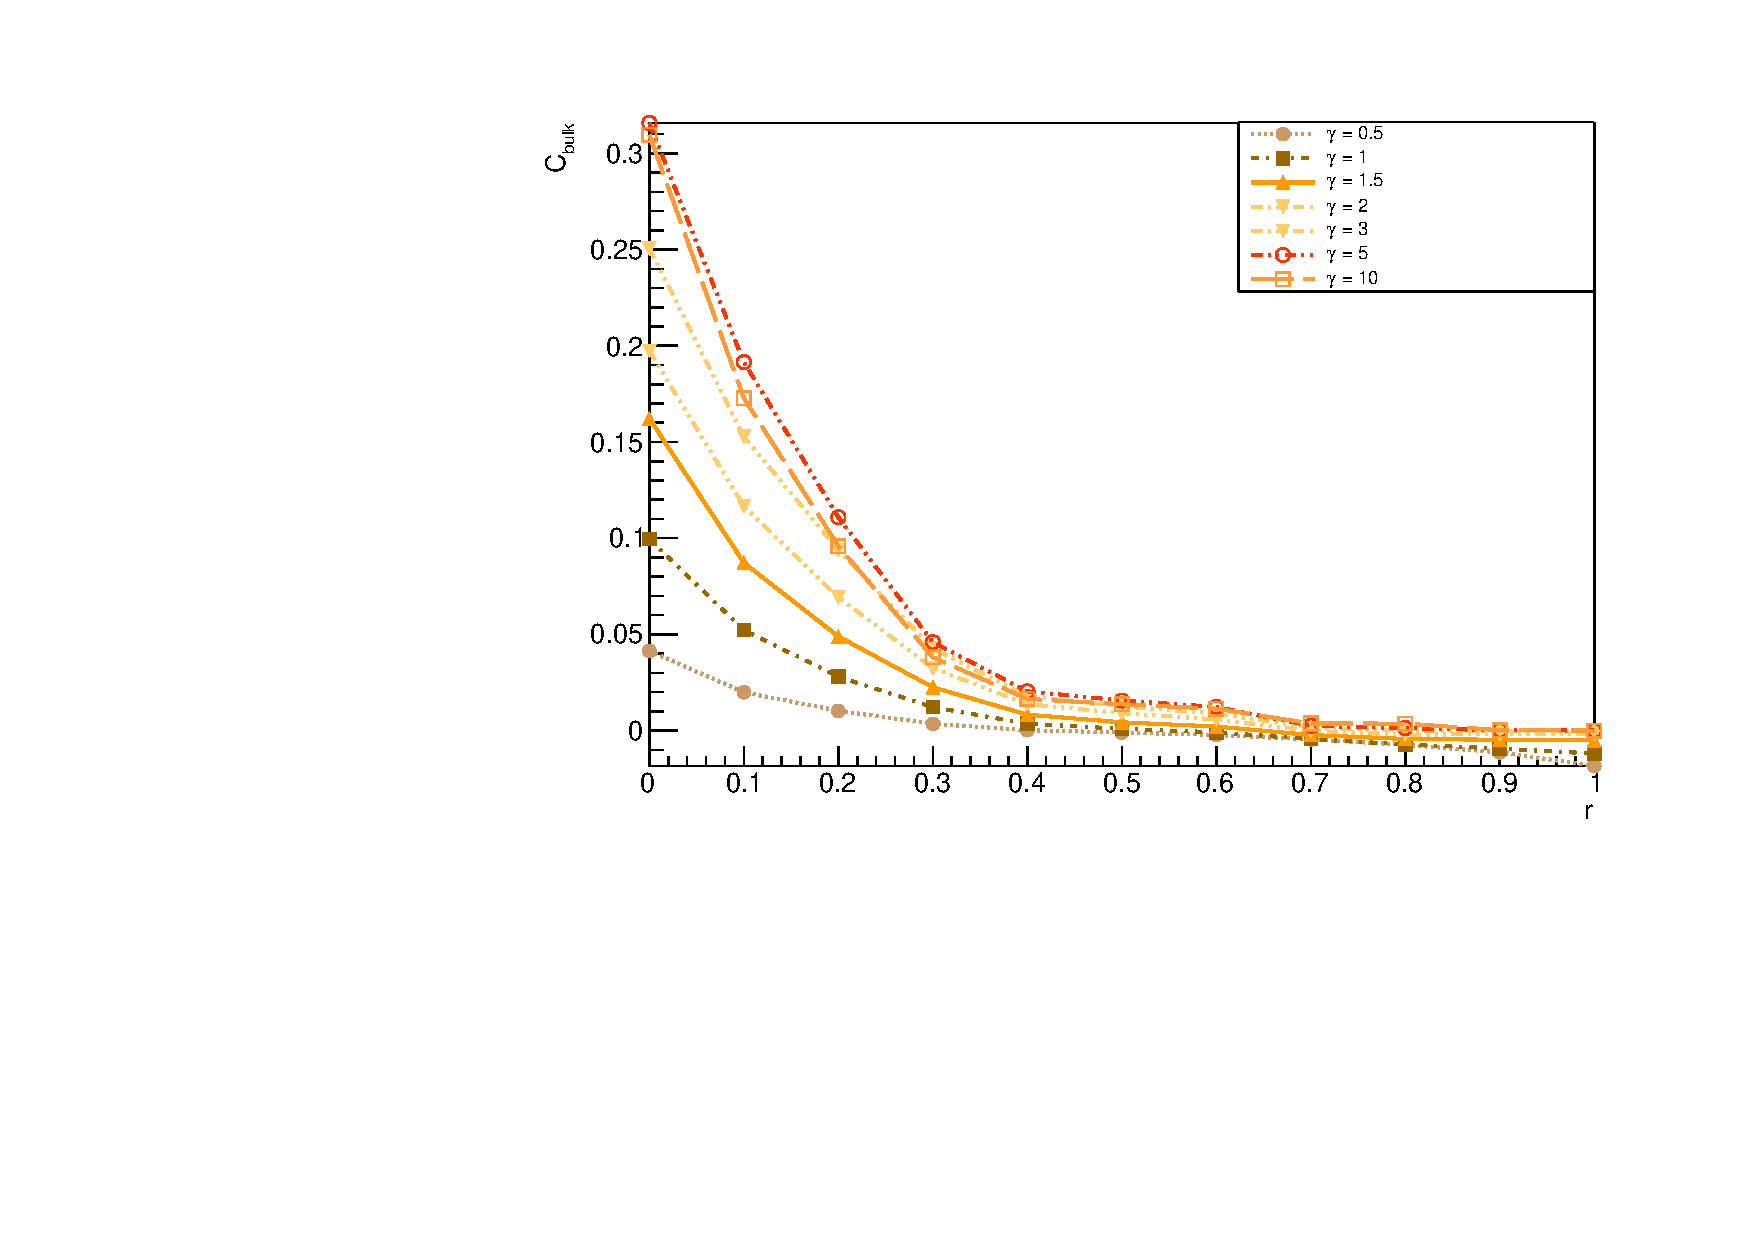
\includegraphics[scale=0.7]{Figures/12sites/12sites_CFBulkCONNVSgamma.pdf}
    \captionsetup{width=1.\linewidth}
    \caption{Bulk correlation function for a 12-sites spin chain. Data are obtained from MPO method.}
    \label{fig:12sites_CFBulkCONNVSgamma}
\end{figure}

\begin{figure}[H]
    \centering
    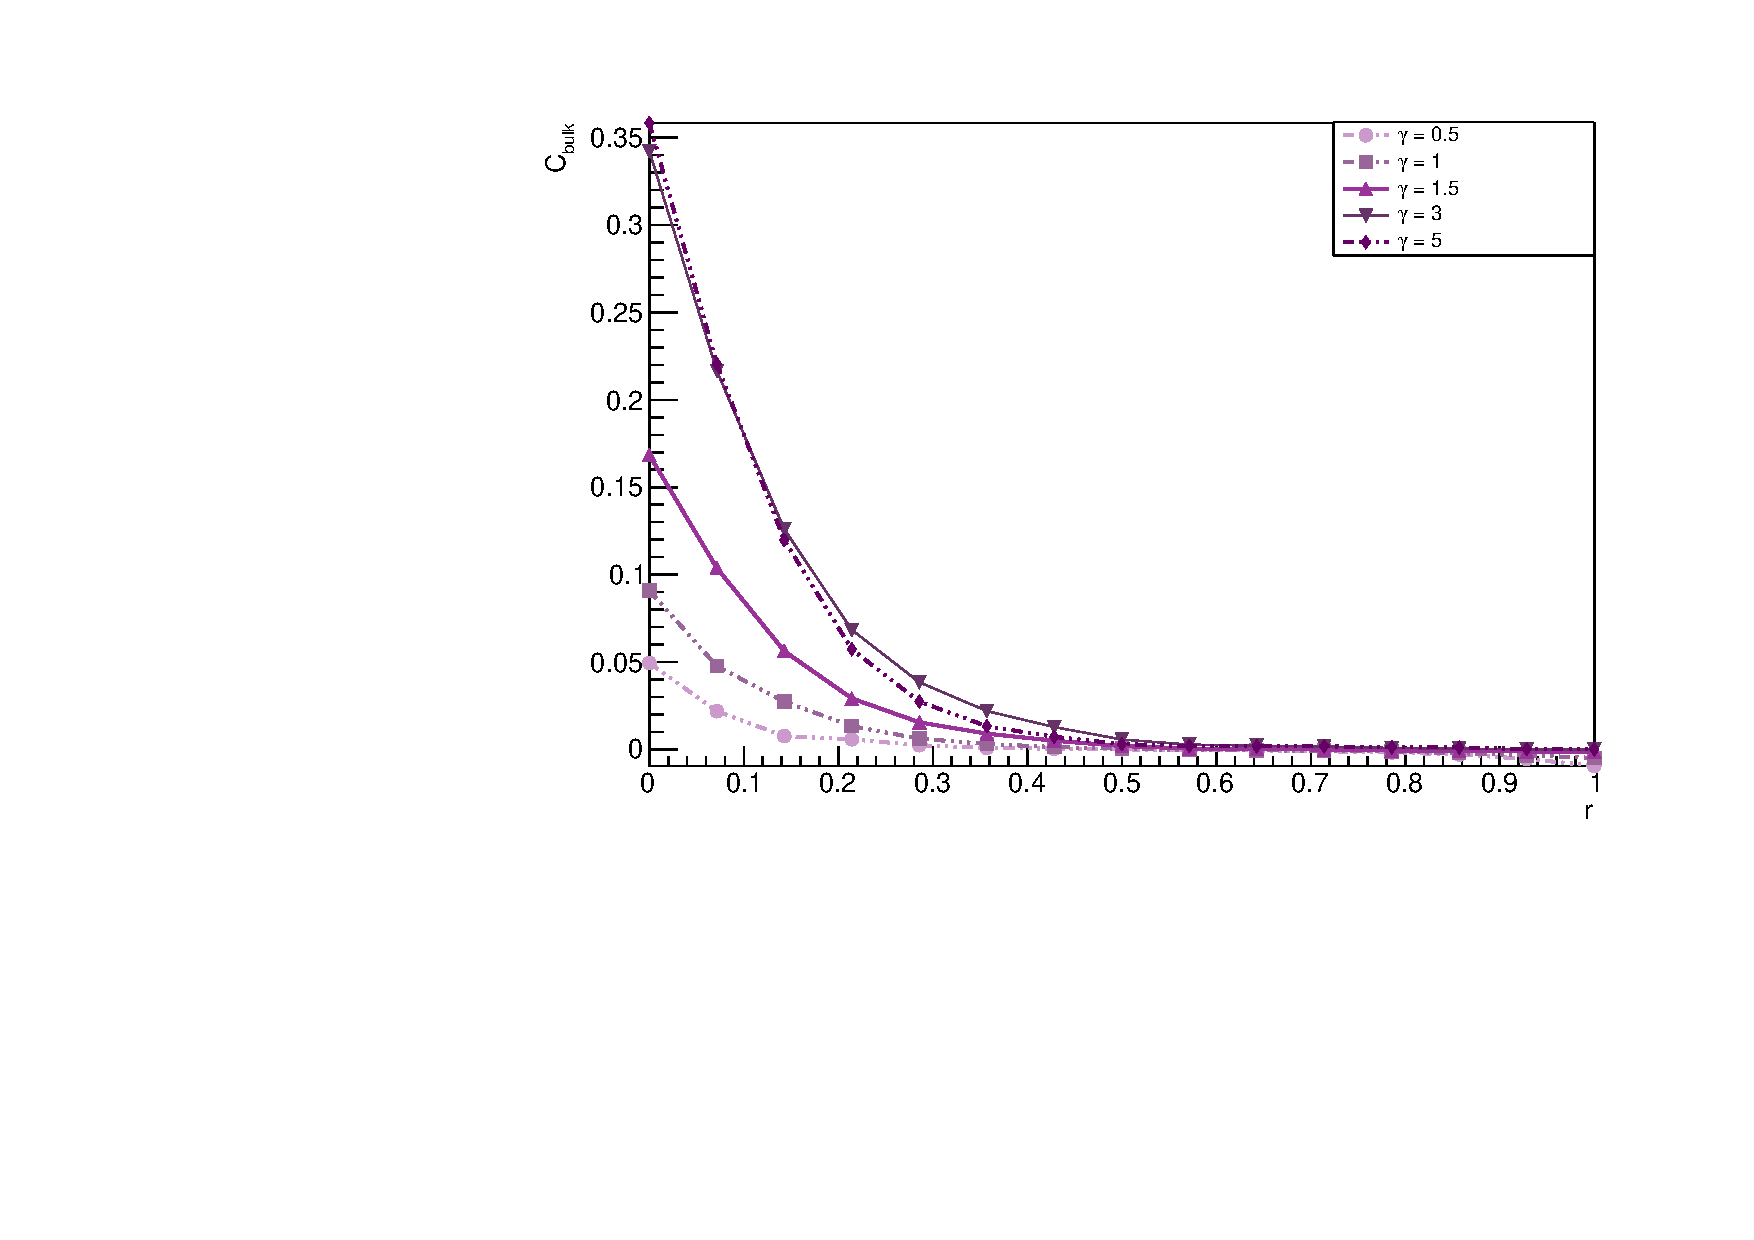
\includegraphics[scale=0.7]{Figures/16sites/16sites_CFBulkCONNVSgamma.pdf}
    \captionsetup{width=1.\linewidth}
    \caption{Bulk correlation function for a 16-sites spin chain. Data are obtained from MPO method.}
    \label{fig:16sites_CFBulkCONNVSgamma}
\end{figure}

The fit made with~\cite{root_cern} shows that the profile of correlation function is exponential. In fig.~\ref{fig:16sites_FIT_CFBulkCONNvsGamma} several observations can be made; first of all, the trend of the two-point correlation function is exponential. In particular, the dependence from the distance between the spin reads:
\begin{equation*}
    C(r) = p_0 e^{-p_1 r},
\end{equation*}
where the coefficients $p_0$ and $p_1$ are given by the fit and are displayed in fig.~\ref{fig:16sites_FIT_CFBulkCONNvsGamma}. Here, we can see that the correlation between nearest neighbours (i.e. the first point of every curve) gets bigger as $\gamma$ grows.

\begin{figure}[H]
    \centering
    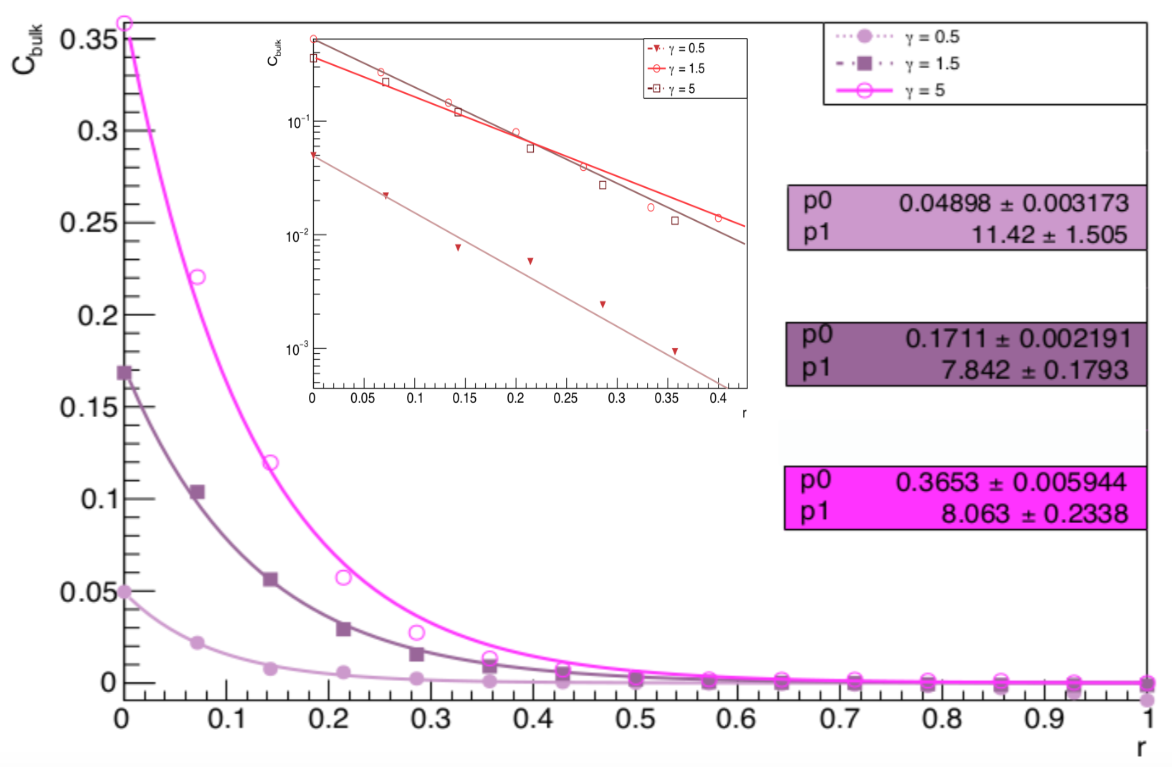
\includegraphics[scale=0.7]{Figures/16sites/16sites_FIT_CFBulkCONNvsGamma.png}
    \captionsetup{width=1.\linewidth}
    \caption{Bulk correlation function for a 16-sites spin chain for several values of $\gamma$. It is shown the fit $C_{\text{bulk}} = p_0 \exp{(-p_1 r)}$. The fit parameters are show in the same order of the legend for $\gamma$. In the box there is the same fit in a semi-logarithmic scale.}
    \label{fig:16sites_FIT_CFBulkCONNvsGamma}
\end{figure}

%\textcolor{red}{Add the comparison bet MPO and QT.}

%%%%%%%%%%%%%%%%%%%%%%%%%%%%%%%%%%%%%%%%%%%%%%%%%%%%%%%%%%%%%%%%%%%%%%%%%%%%%%%%%%%%%%%%%%%%%%%%%%%%%%%%%%%%%%%%%%%%%%%%%%%%%%%%%%%%%%%%%%%%%%%%%%%%%%%%%%%%%%%%%%%%%%%%%%%%%%%%%%%%%%%%%%%%%%%%%%%%%%%%%%%%%%%%%%%%%%%%%%%%%%%%%%%%%%%%%%%%%%%%%%%%%%%%%%%%%%%%%%
\section{Spin Transport}
In this section we are going to study the spin current $j_\sigma$ defined from the continuity equation for the local spin operators~\cite{BenentiCasatiProsenRossini}:
\begin{equation}
    \frac{\partial S^k_z}{\partial t} + \nabla (j_\sigma)_k = 0,
\end{equation}
which can be rewritten as
\begin{equation}
    (j_\sigma)_{k+1}-(j_\sigma)_k = \frac{i}{2}[\sigma_k^z , H],
\end{equation}
where $S_k^z \equiv \sigma_k^z/2$ and where $H$ is the Hamiltonian written in~\ref{ham_chain}. So, we obtain:
\begin{equation}
    j_\sigma = J_y (\sigma_k^x \sigma_{k+1}^y) - J_x (\sigma_k^y \sigma_{k+1}^x). 
\end{equation}


%\begin{figure}[H]
    %\centering
    %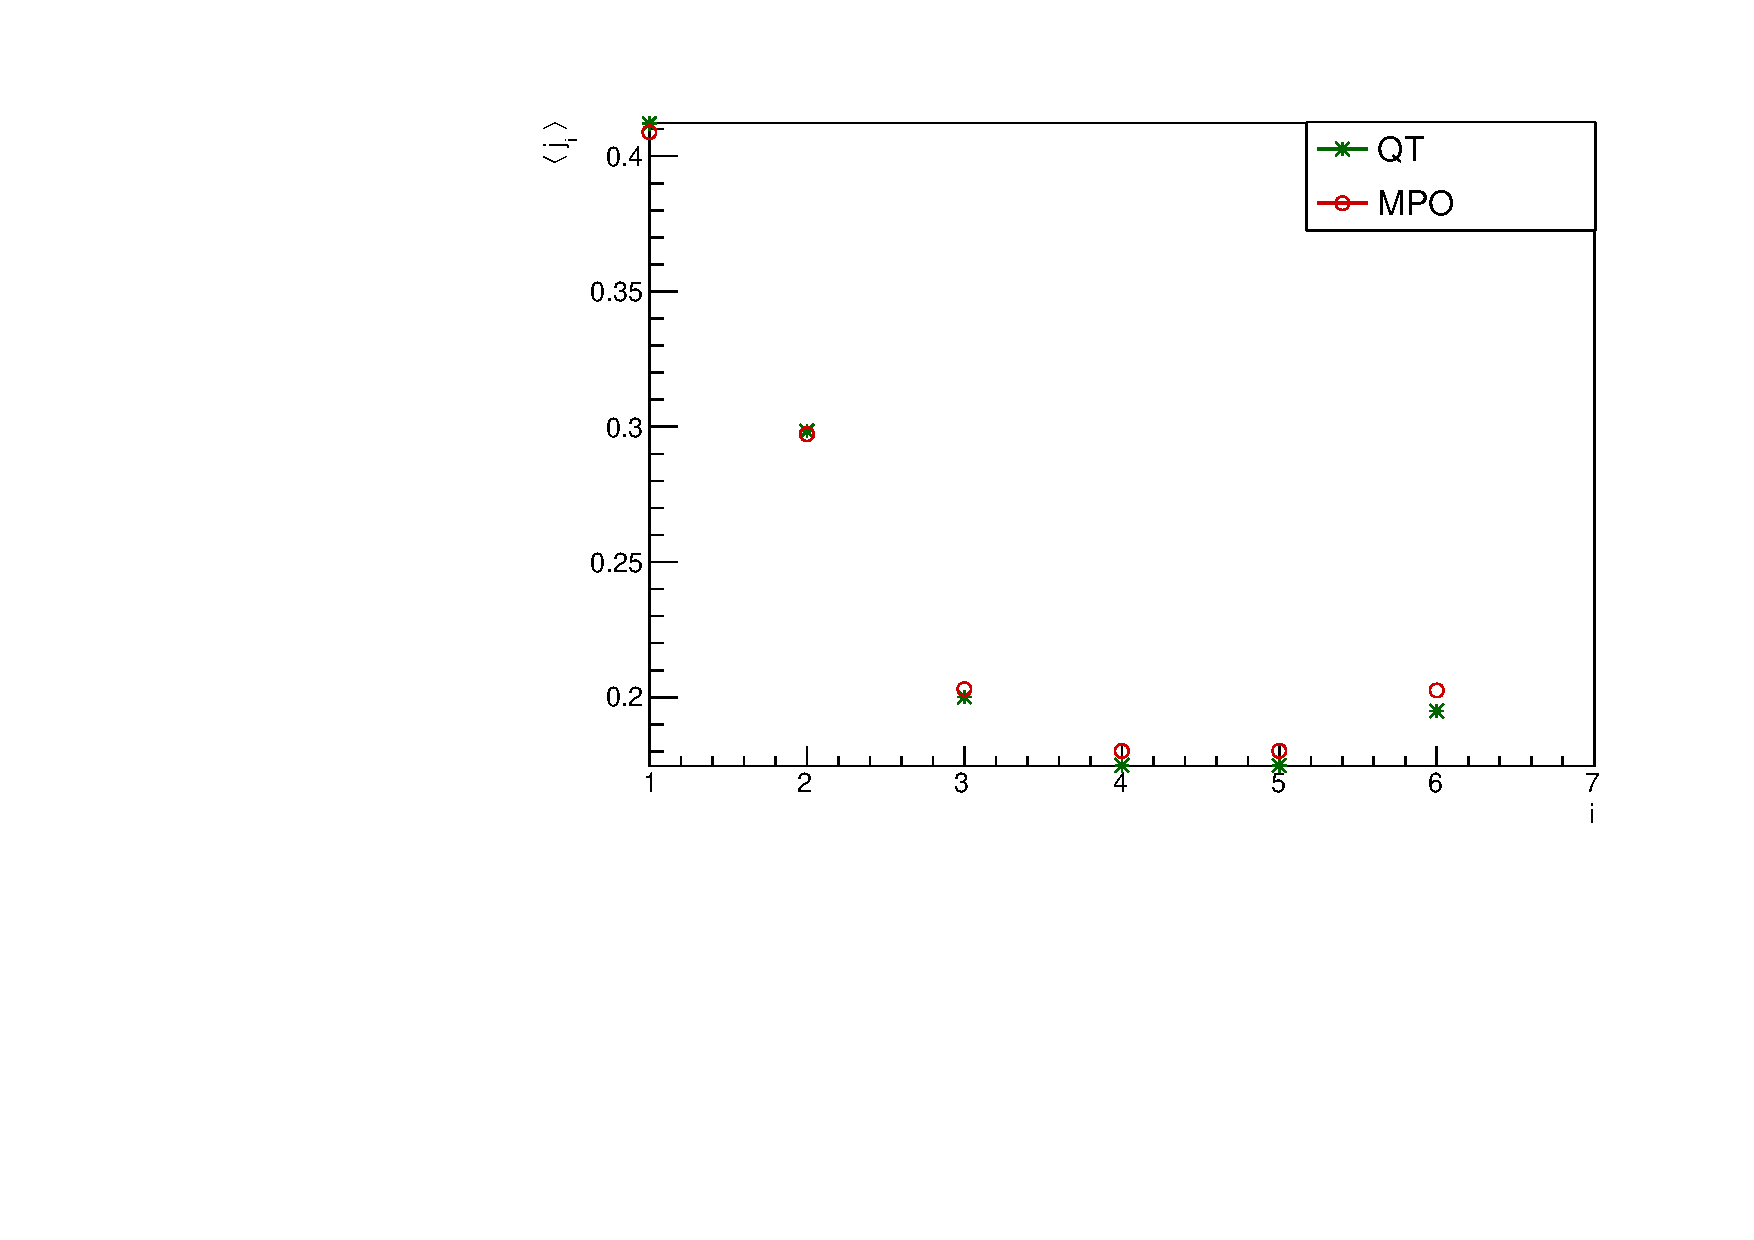
\includegraphics[scale=0.7]{Figures/8sites/SpinCurr_8s_J10505.pdf}
    %\caption{Spin current of the chain, characterized by $\gamma=1, J_x=1, J_y=0.5, %J_z=0.5$; \emph{i} stands for the site index.}
    %\label{fig:my_label}
%\end{figure}

%\begin{figure}[H]
    %\centering
    %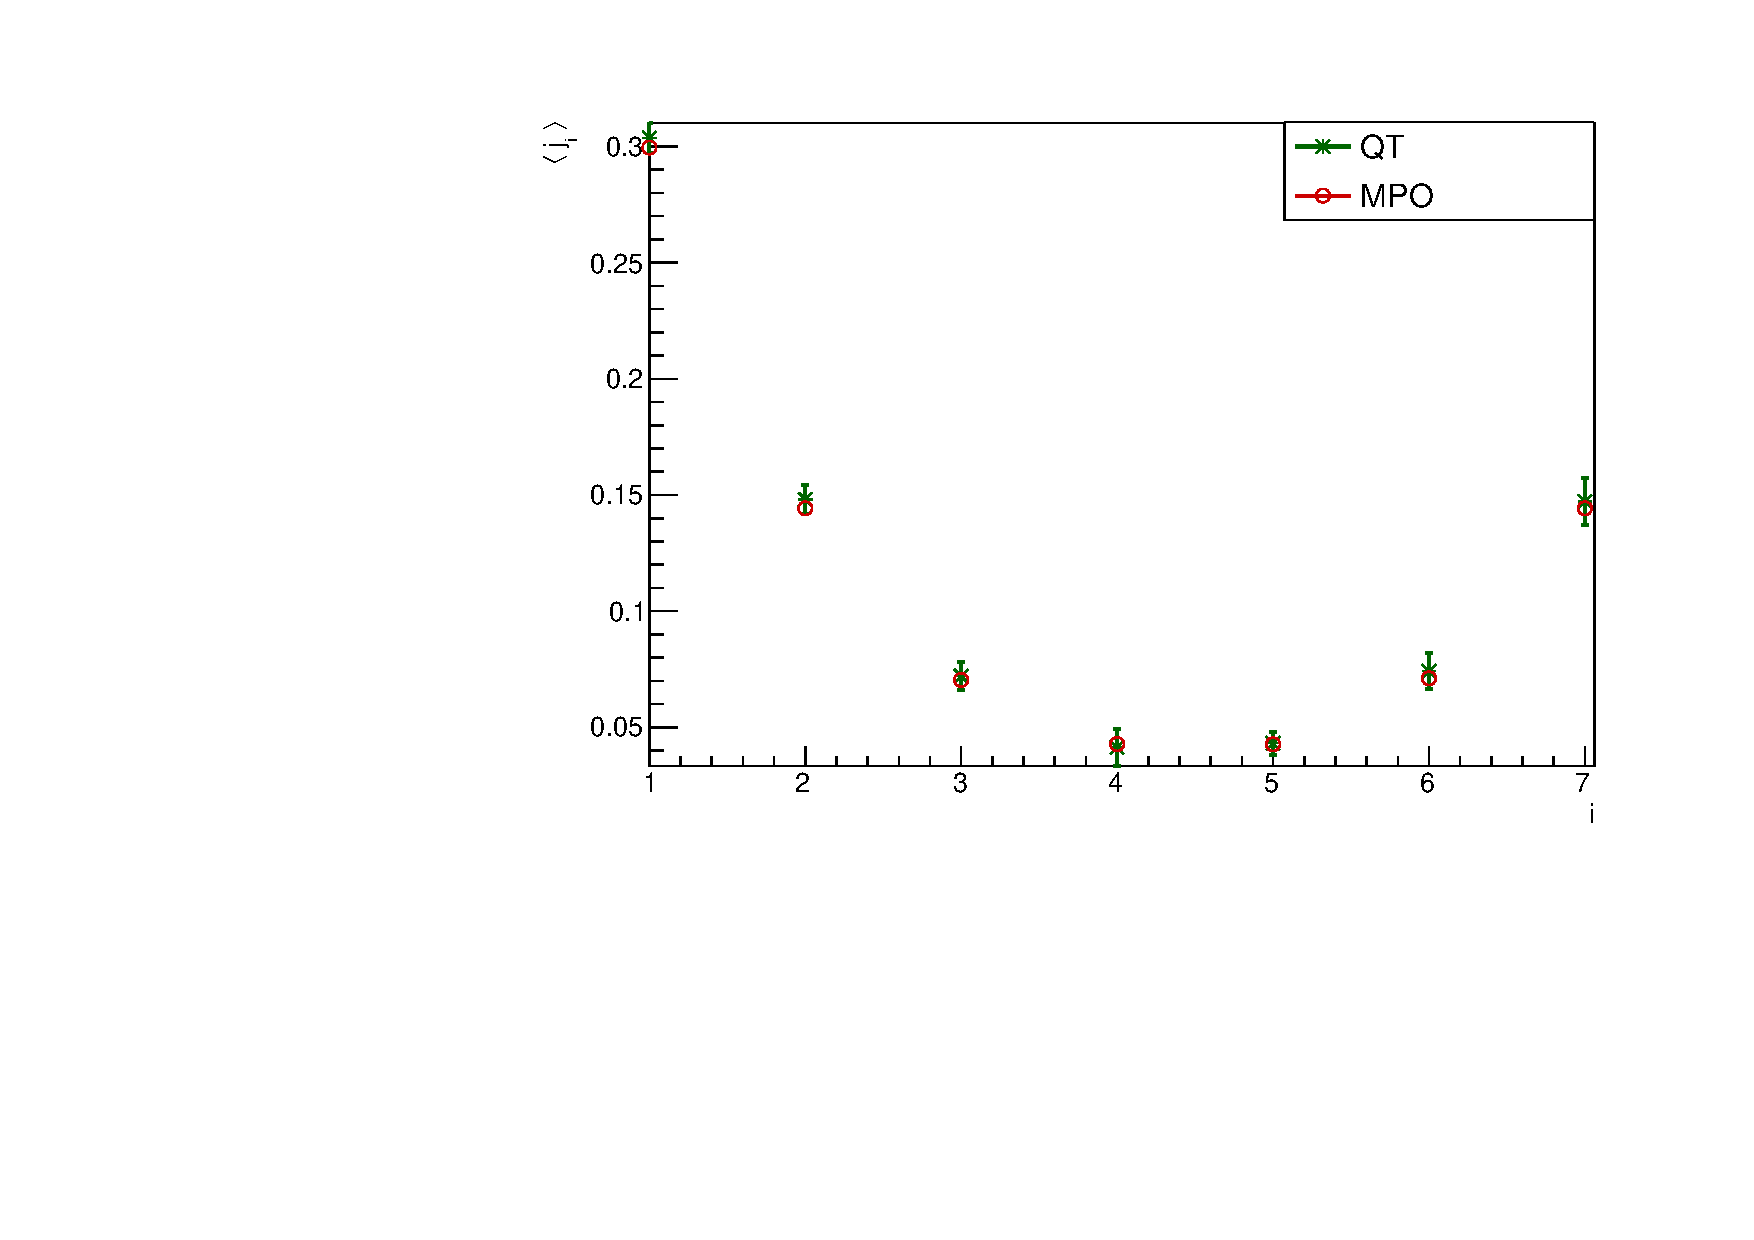
\includegraphics[scale=0.7]{Figures/8sites/SpinCurr_8s_J1051.pdf}
    %\caption{Spin current of the chain, characterized by $\gamma=1, J_x=1, J_y=0.5, %J_z=1$; \emph{i} stands for the site index.}
    %\label{fig:my_label}
%\end{figure}

%\begin{figure}[H]
    %\centering
    %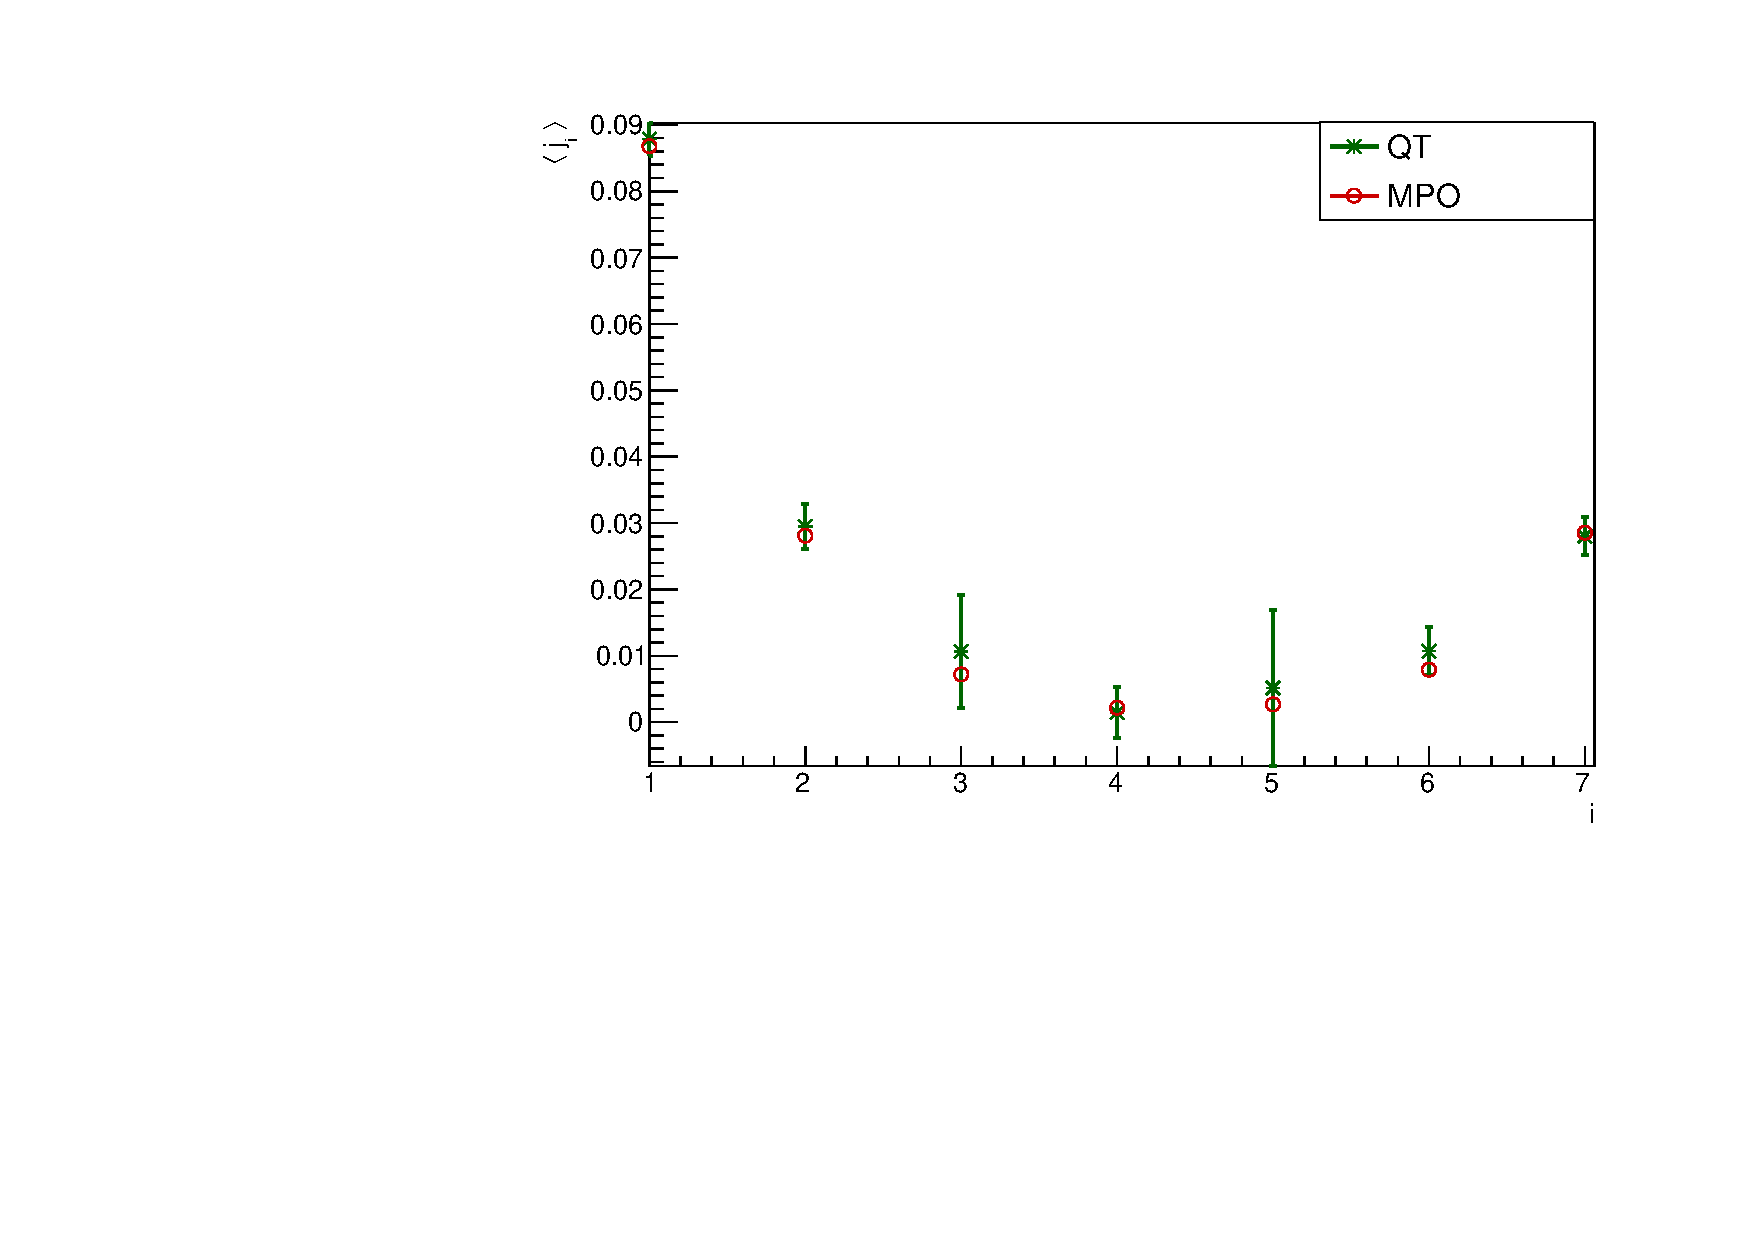
\includegraphics[scale=0.7]{Figures/8sites/SpinCurr_8s_J10515.pdf}
    %\caption{Spin current of the chain, characterized by $\gamma=1, J_x=1, J_y=0.5, %J_z=1.5$; \emph{i} stands for the site index.}
    %\label{fig:my_label}
%\end{figure}

%Let us see what happens in the case of a \textbf{12-sites} chain.
%
%\begin{figure}[H]
%    \centering
%    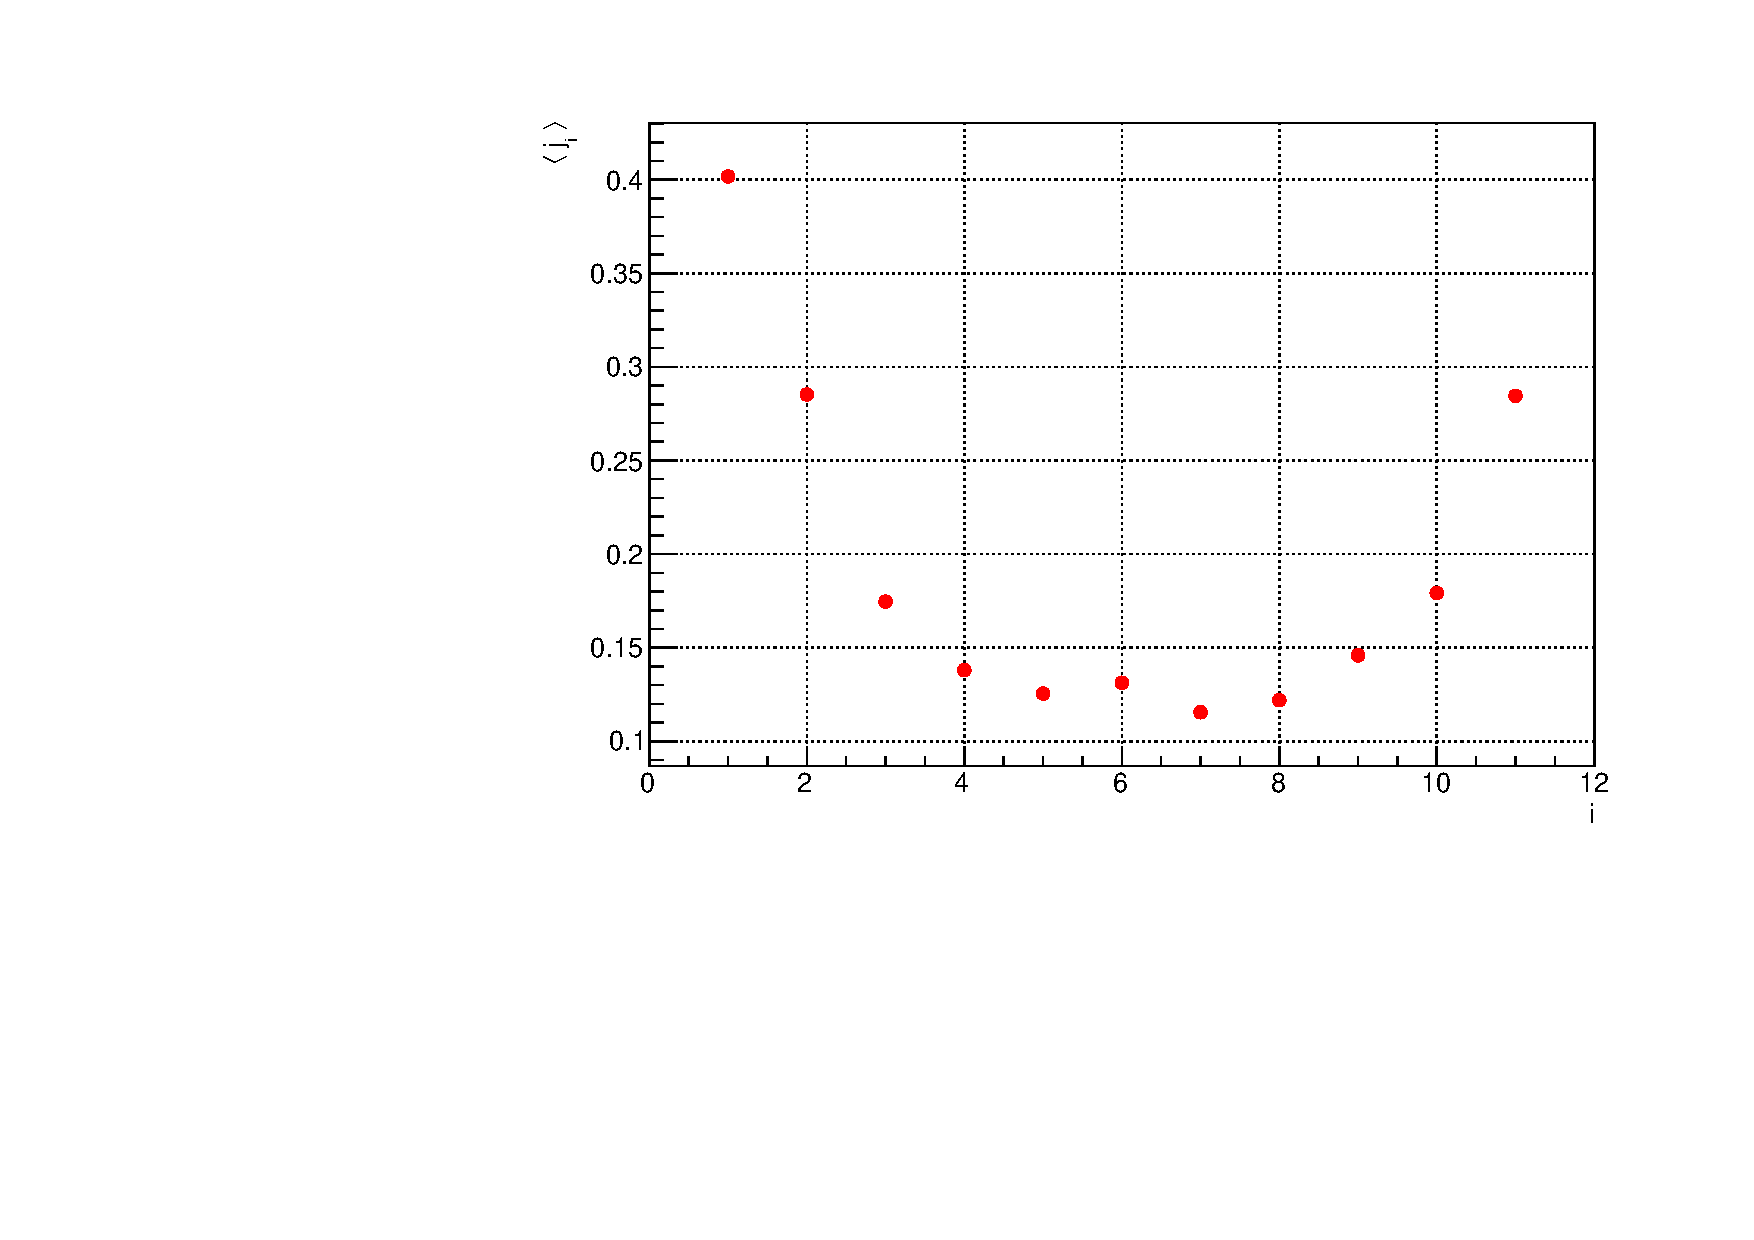
\includegraphics[scale=0.7]{Figures/12sites/SpinCurrL012m060Time002000_J10505.pdf}
%    \caption{Spin current of a 12-sites chain, characterized by $\gamma=1, J_x=1, J_y=0.5, J_z=0.5$; %\emph{i} stands for the site index. Data are obtained from MPO method.}
%    \label{fig:my_label}
%\end{figure}
%
%\begin{figure}[H]
%    \centering
%    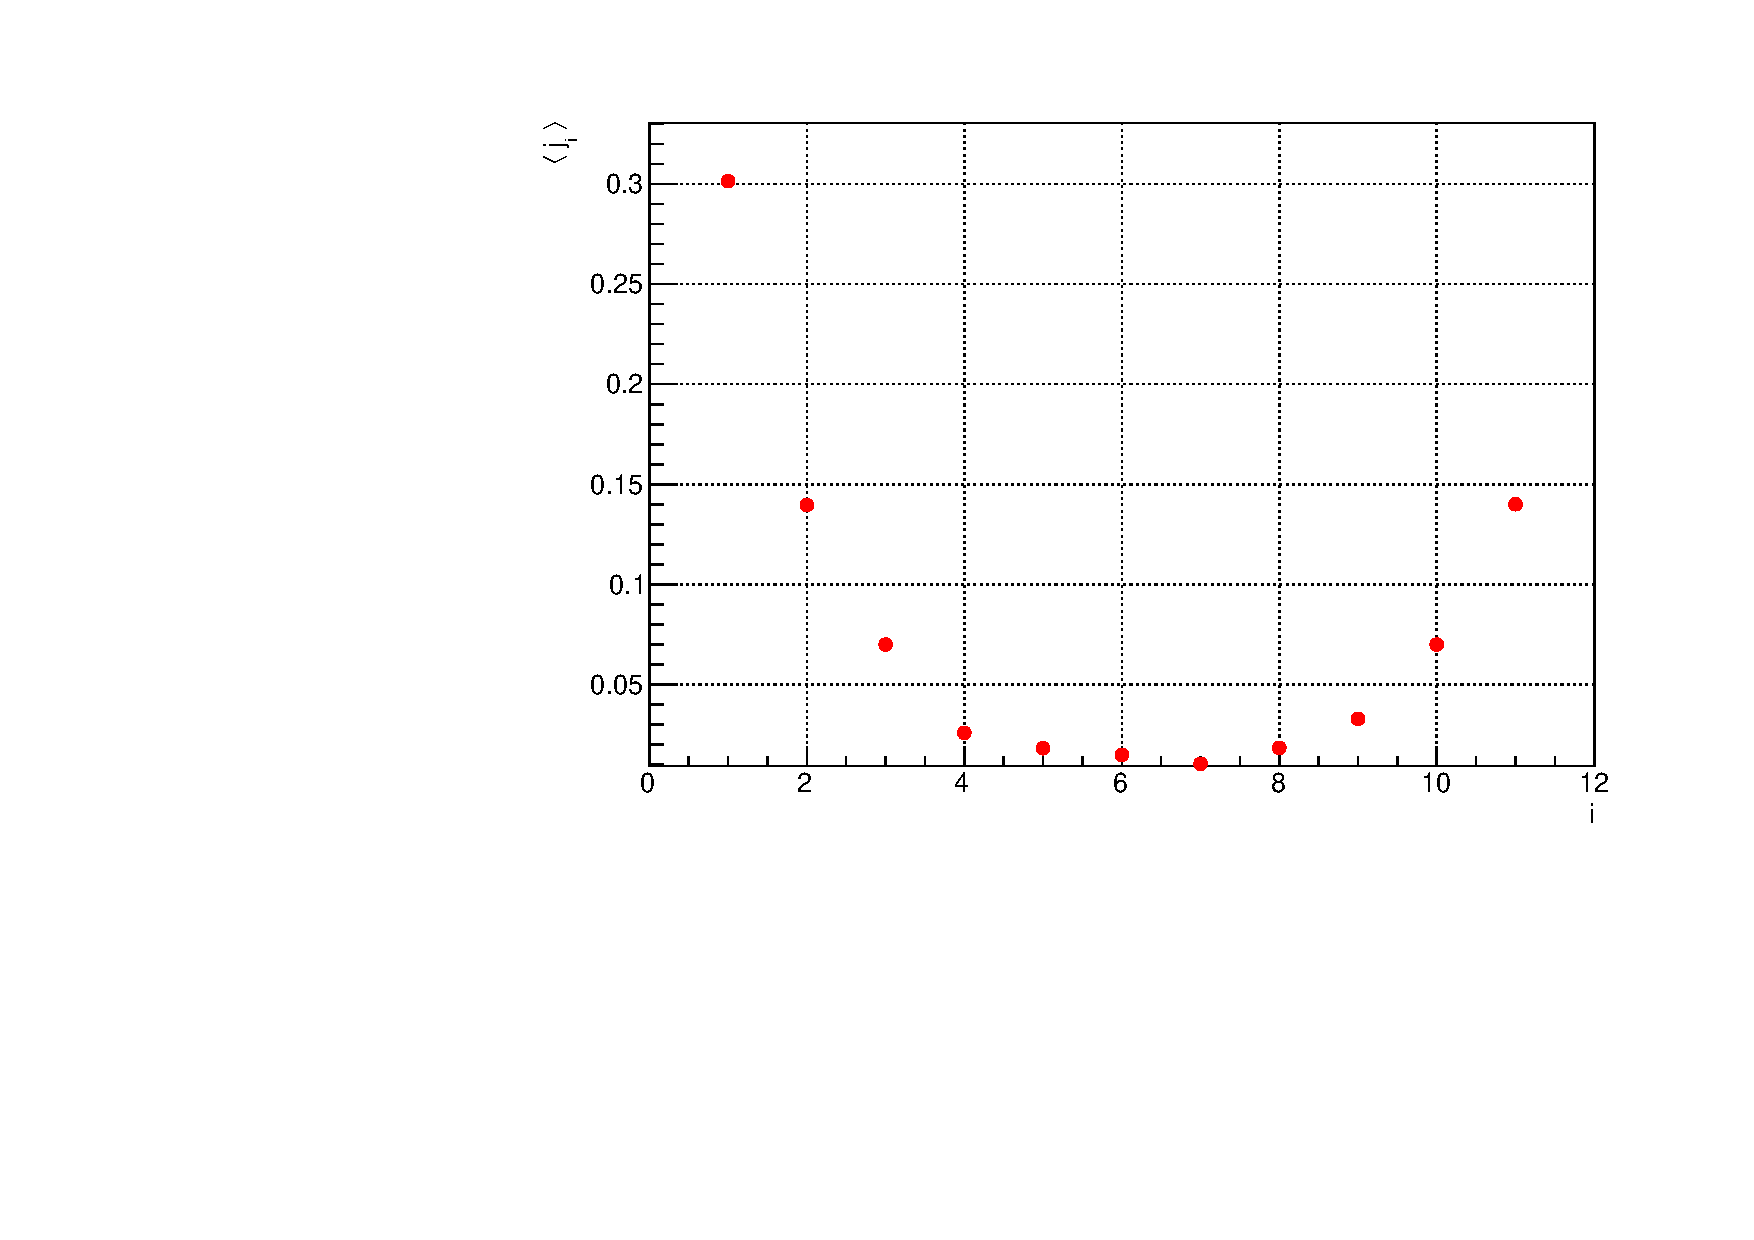
\includegraphics[scale=0.7]{Figures/12sites/SpinCurrL012m060Time002000_J1051.pdf}
%    \caption{Spin current of a 12-sites chain, characterized by $\gamma=1, J_x=1, J_y=0.5, J_z=1.$; %\emph{i} stands for the site index. Data are obtained from MPO method.}
%    \label{fig:my_label}
%\end{figure}
%
%\begin{figure}[H]
%    \centering
%    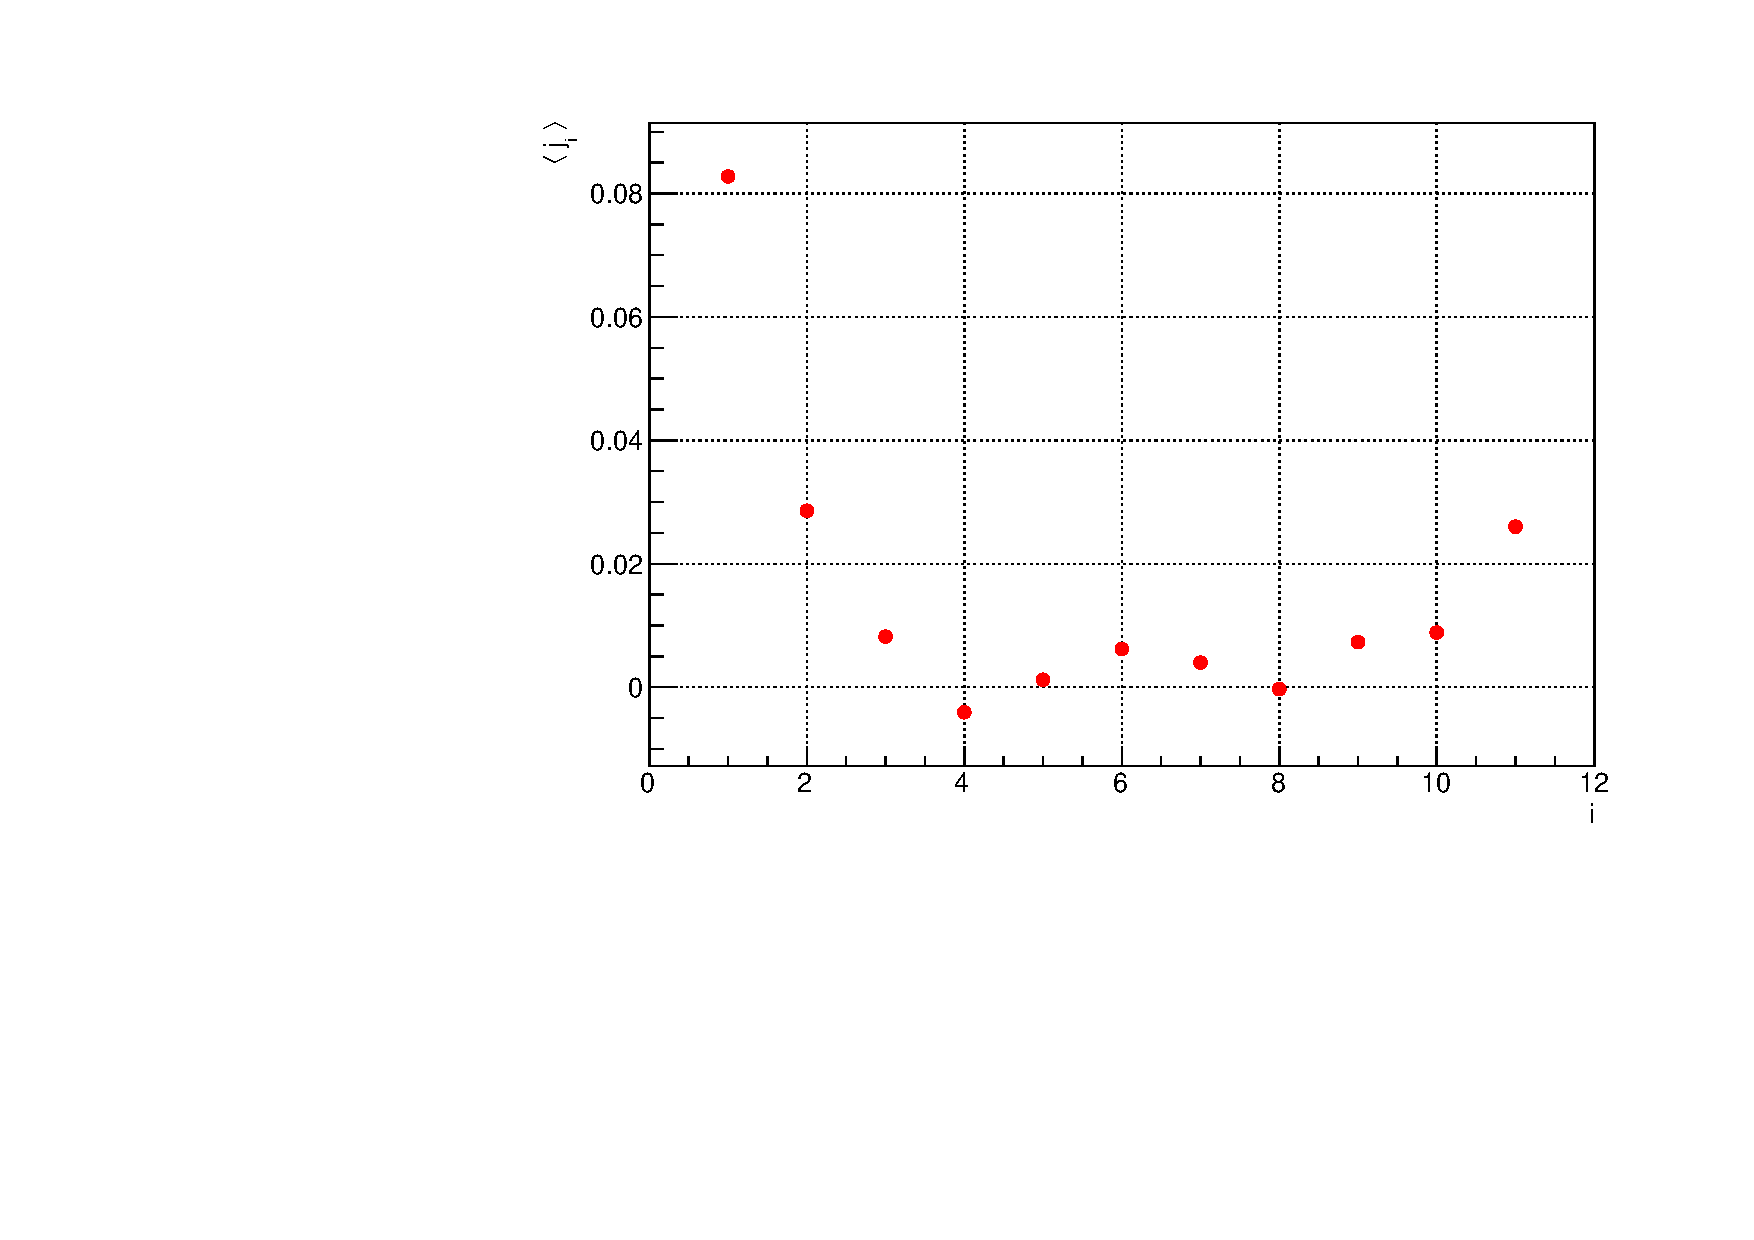
\includegraphics[scale=0.7]{Figures/12sites/SpinCurrL012m060Time002000_J10515.pdf}
%    \caption{Spin current of a 12-sites chain, characterized by $\gamma=1, J_x=1, J_y=0.5, J_z=1.5$; %\emph{i} stands for the site index. Data are obtained from MPO method.}
%    \label{fig:my_label}
%\end{figure}

As done previously for the observables already studied, we can see how the spin current changes for chain of different lengths with the same model. In fig.~\ref{fig:NORM_SpinCurr_comparisonVSsize} it is shown the spin current for a 8, 12 and 16-sites chain, characterized by $J_z = 1$ and dissipation rate $\gamma = 1$. The curves are asymmetric, due to the fact that the Heisenberg model XYZ has an intrinsic anisotropy. While the length of the chain increases, the spin current shows a flatter profile which is consistent with the fig.~\ref{fig:LM_comparisonVSsizeJz1Gamma1} where the plateau of null magnetization becomes bigger while the size of the chain grows.

\begin{figure}[H]
    \centering
    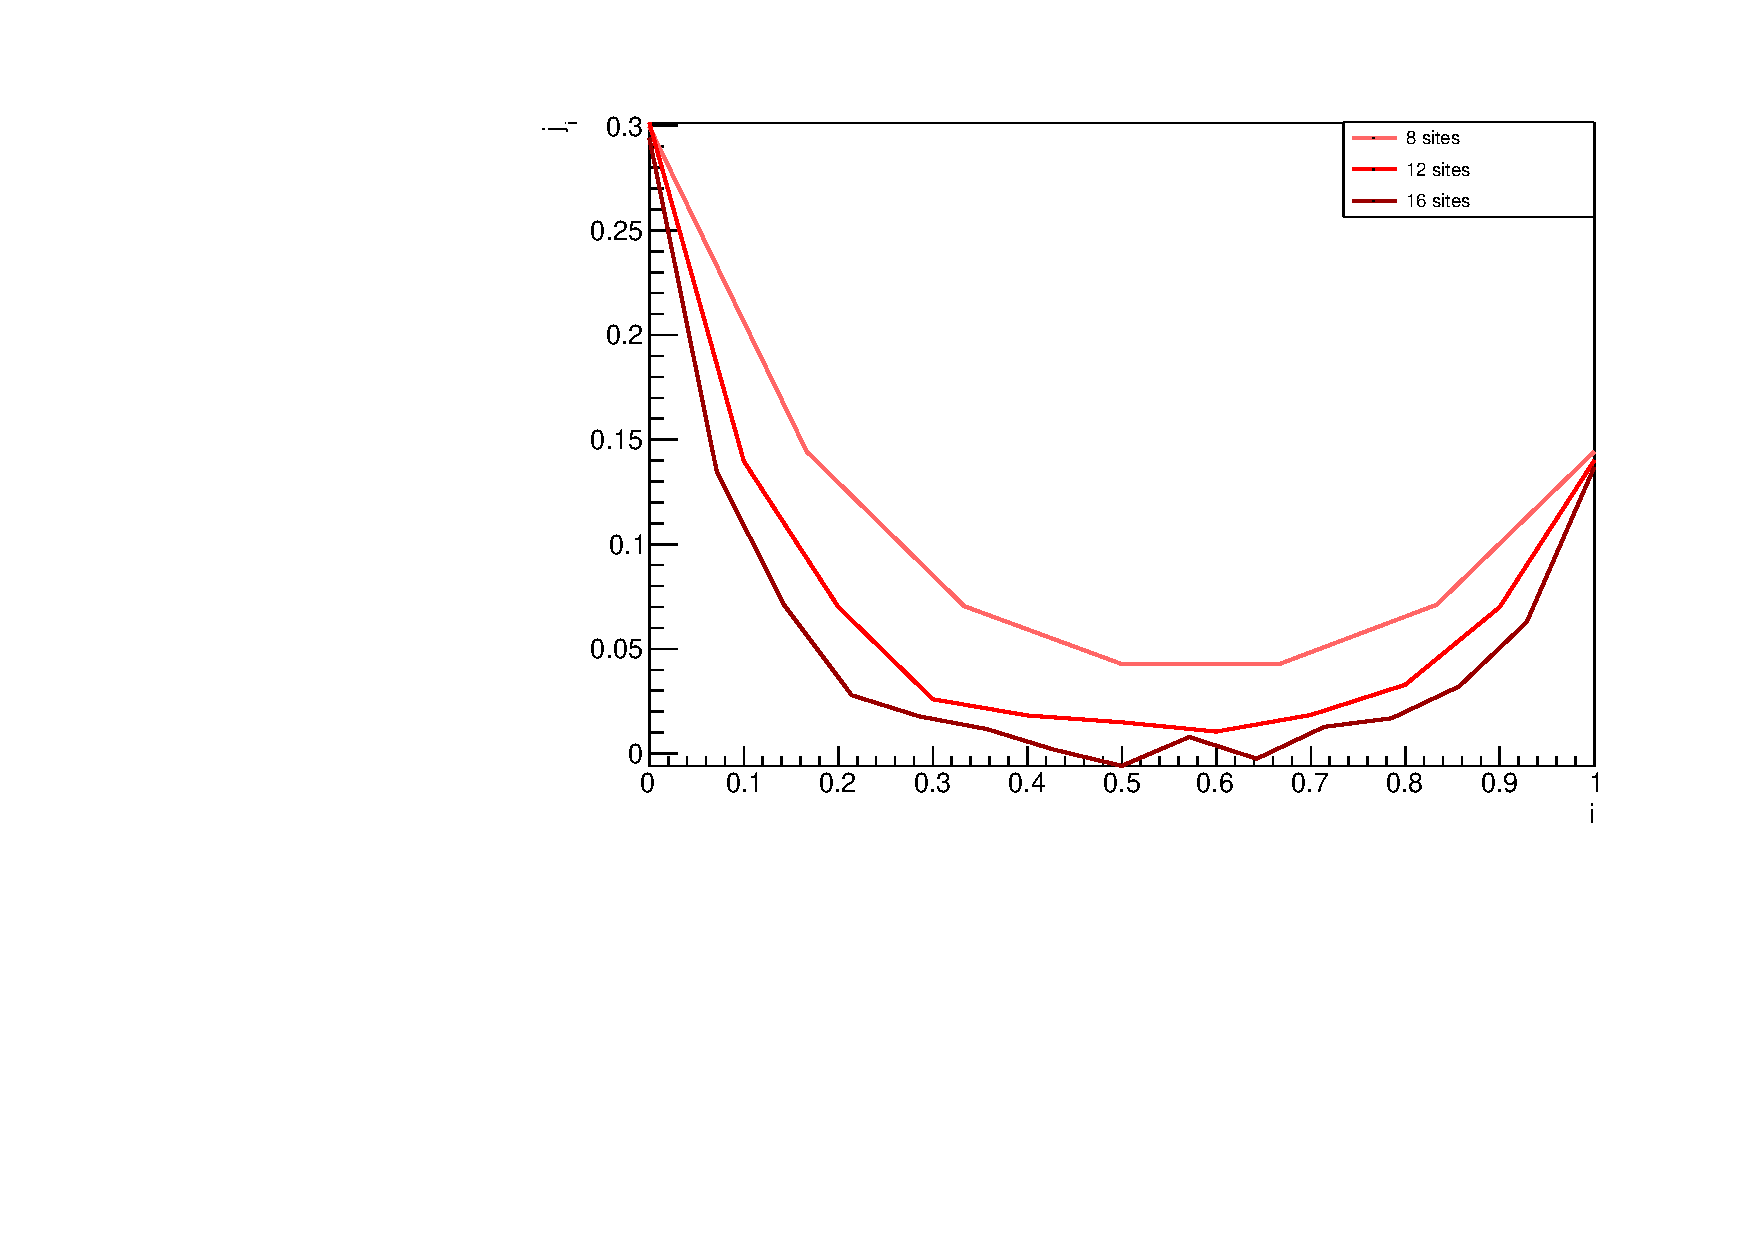
\includegraphics[scale=0.7]{Figures/NORM_SpinCurr_comparisonVSsize.pdf}
    \captionsetup{width=1.\linewidth}
    \caption{Spin current for the model at $J_z = 1$. Data for different chain lengths are shown. They are obtained from MPO method.}
    \label{fig:NORM_SpinCurr_comparisonVSsize}
\end{figure}

An aspect worth considering is the common peak value of the spin current, independent of the chain size. As done in the section~\ref{sec:magn_profile} studying the magnetization profile, we can see how this value changes varying $\gamma$. 

\begin{figure}[H]
    \centering
    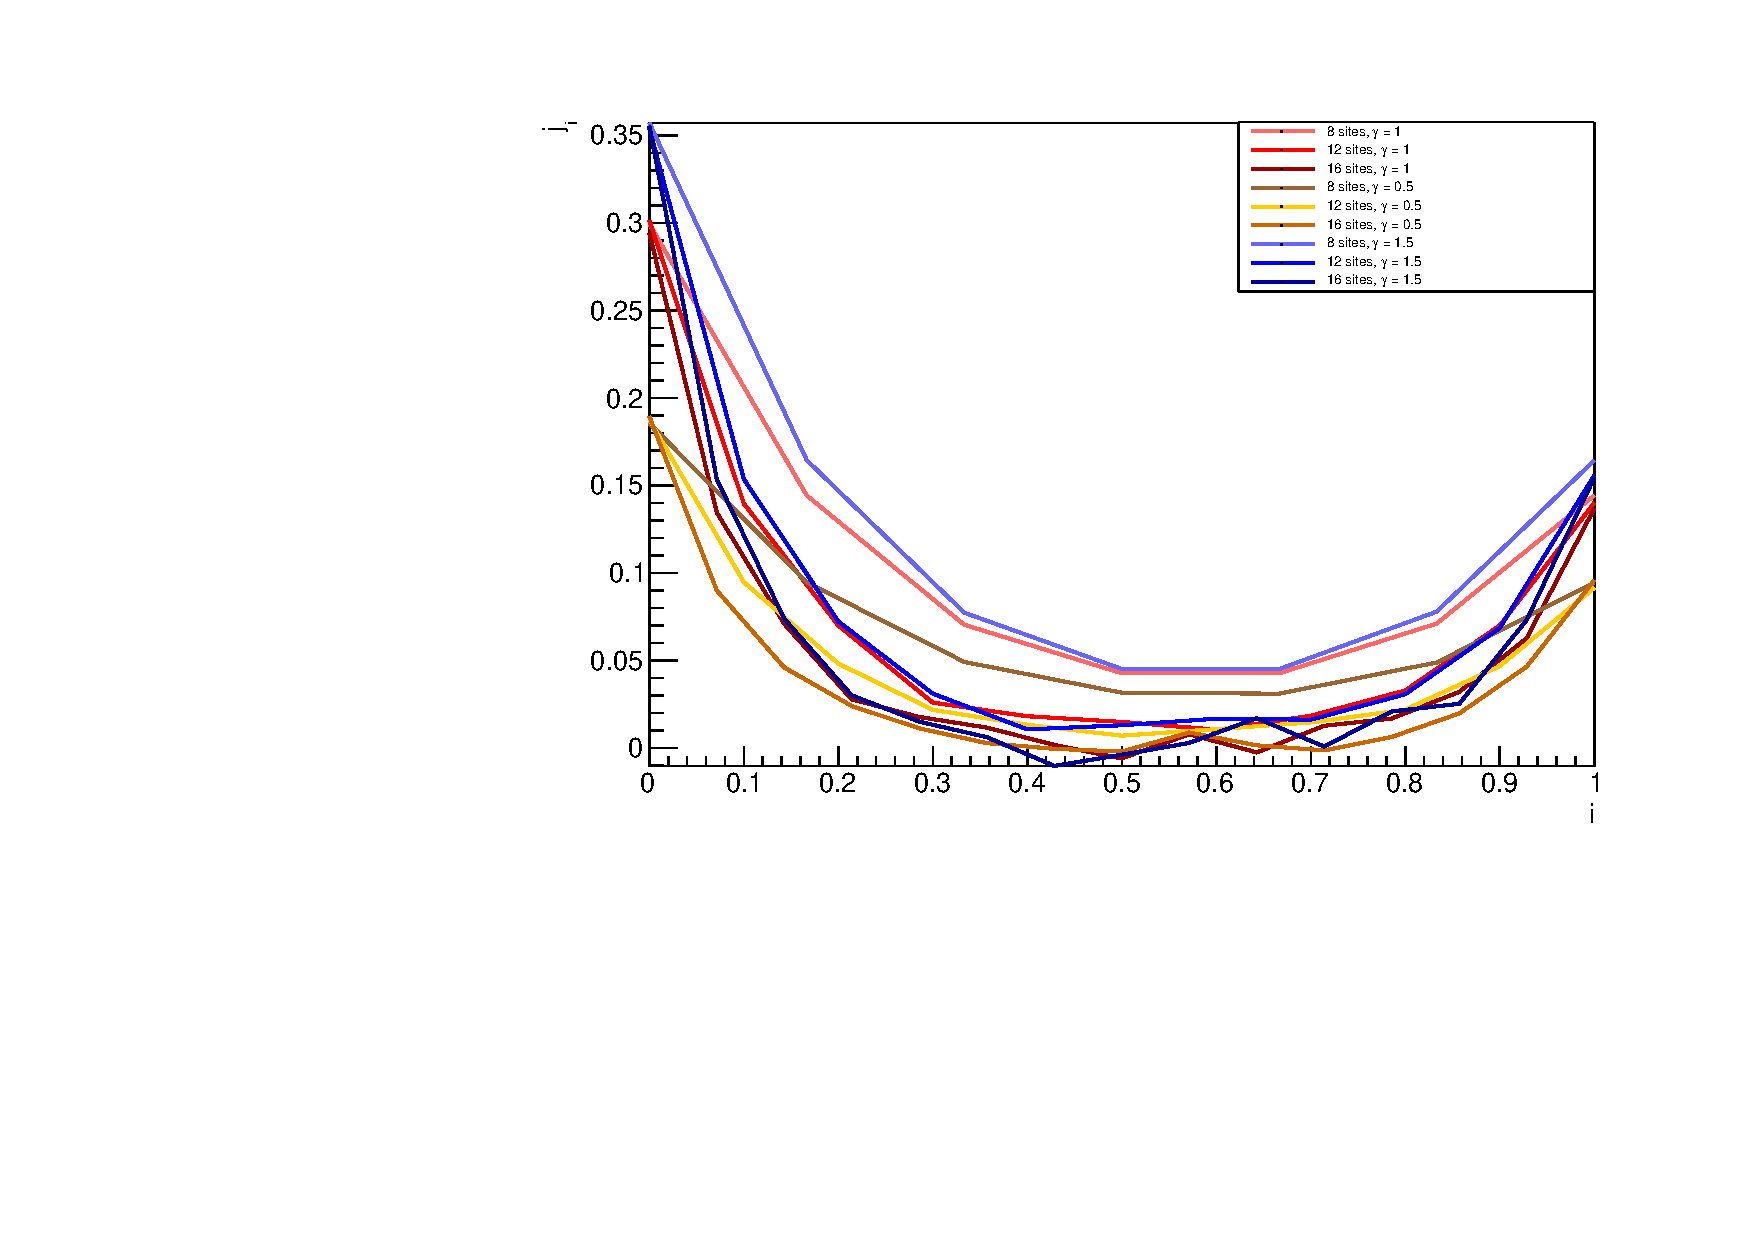
\includegraphics[scale=0.7]{Figures/SpinCurrcomparisonVSsizeANDdissipationRate.pdf}
    \caption{Spin current for the model at fixed $J_z = 1$, for several values of $\gamma$.}
    \label{fig:SpinCurrcomparisonVSsizeANDdissipationRate}
\end{figure}

It is interesting noting that the peak values reach a maximum and then decrease, as shown in fig.~\ref{fig:PeakValueSpinCurrVSgamma_8sites}. This can be explained analyzing the curve. First of all, for small values (i.e. $\gamma \sim 0.5$) there is a non-null spin current; as said, for a certain value of $\gamma$ the spin current reaches the maximum value and then begins to decrease tending asymptotically to zero. While $\gamma$ grows, the dissipation acquires a more important role over the Hamiltonian dynamics, the system is driven so that its spin current is zero. This is consistent with the trend shown in fig.~\ref{fig:FIT_PeakLMvsGamma_J1051} of the positive peak value of $\langle \sigma^z \rangle$ and in fig.~\ref{fig:FIT_16sites_4thSiteVSgamma} of the value of $\langle \sigma^z \rangle$ for the forth site of the chain, in which while $\gamma$ increases the magnetization tends asymptotically to a constant value. 

\begin{figure}[H]
    \centering
    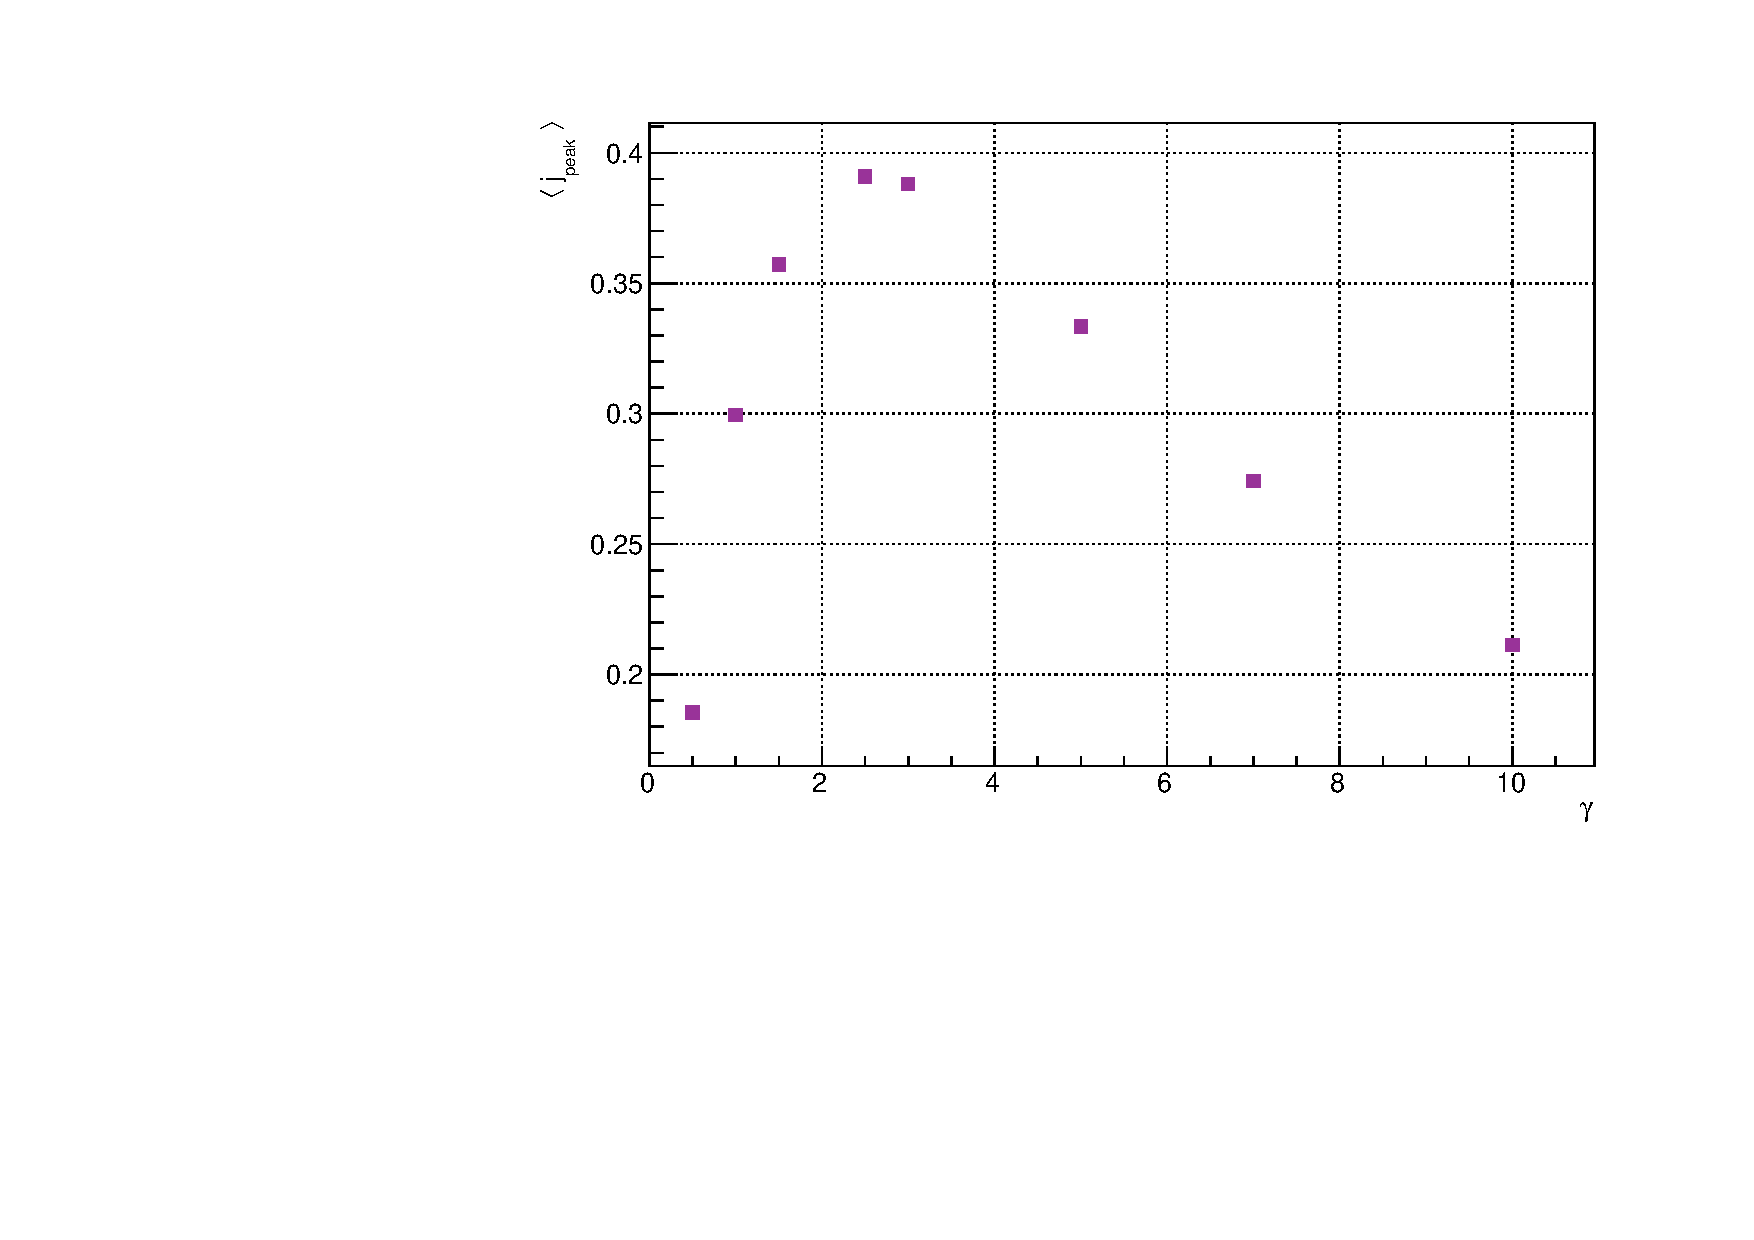
\includegraphics[scale=0.7]{Figures/PeakValueSpinCurrVSgamma_8sites.pdf}
    \captionsetup{width=1.\linewidth}
    \caption{Peak values of spin current for several values of $\gamma$. Data are obtained from MPO method.}
    \label{fig:PeakValueSpinCurrVSgamma_8sites}
\end{figure}


%%%%%%%%%%%%%%%%%%%%%%%%%%%%%%%%%%%%%%%%%%%%%%%%%%%%%%%%%%%%%%%%%%
%%%%%%%%%%%%%%%%%%%%%%%%%%%%%%%%%%%%%%%%%%%%%%%%%%%%%%%%%%%%%%%%%%
%%%%%%%%%%%%%%%%%%%%%%%%%%%%%%%%%%%%%%%%%%%%%%%%%%%%%%%%%%%%%%%%%%
\section{The CSR Method: Limitations and Usability}
The CSR method, described in section~\ref{chapter3_csr}, has been studied and implemented in order to analyze the model described in the last section. The algorithm is written in pseudocode in appendix~\ref{AppendixA}.

In this section, it is shown that the CSR method is not a suitable method for investigating systems described by a model such as the one under consideration.

In order to reveal this, we can easily see the case of a 4-sites chain for the proposed model. In particular, we can study the magnetization profile of the chain, i.e. the steady-state expectation value $\langle \sigma^z \rangle$ of the Pauli spin- matrix $\sigma^z$ for each site:
\begin{equation*}
    \langle \sigma^z \rangle = \Tr(\sigma^z \rho),
\end{equation*}
being $\rho$ the steady-state density matrix of the system.

\begin{figure}[H]
    \centering
    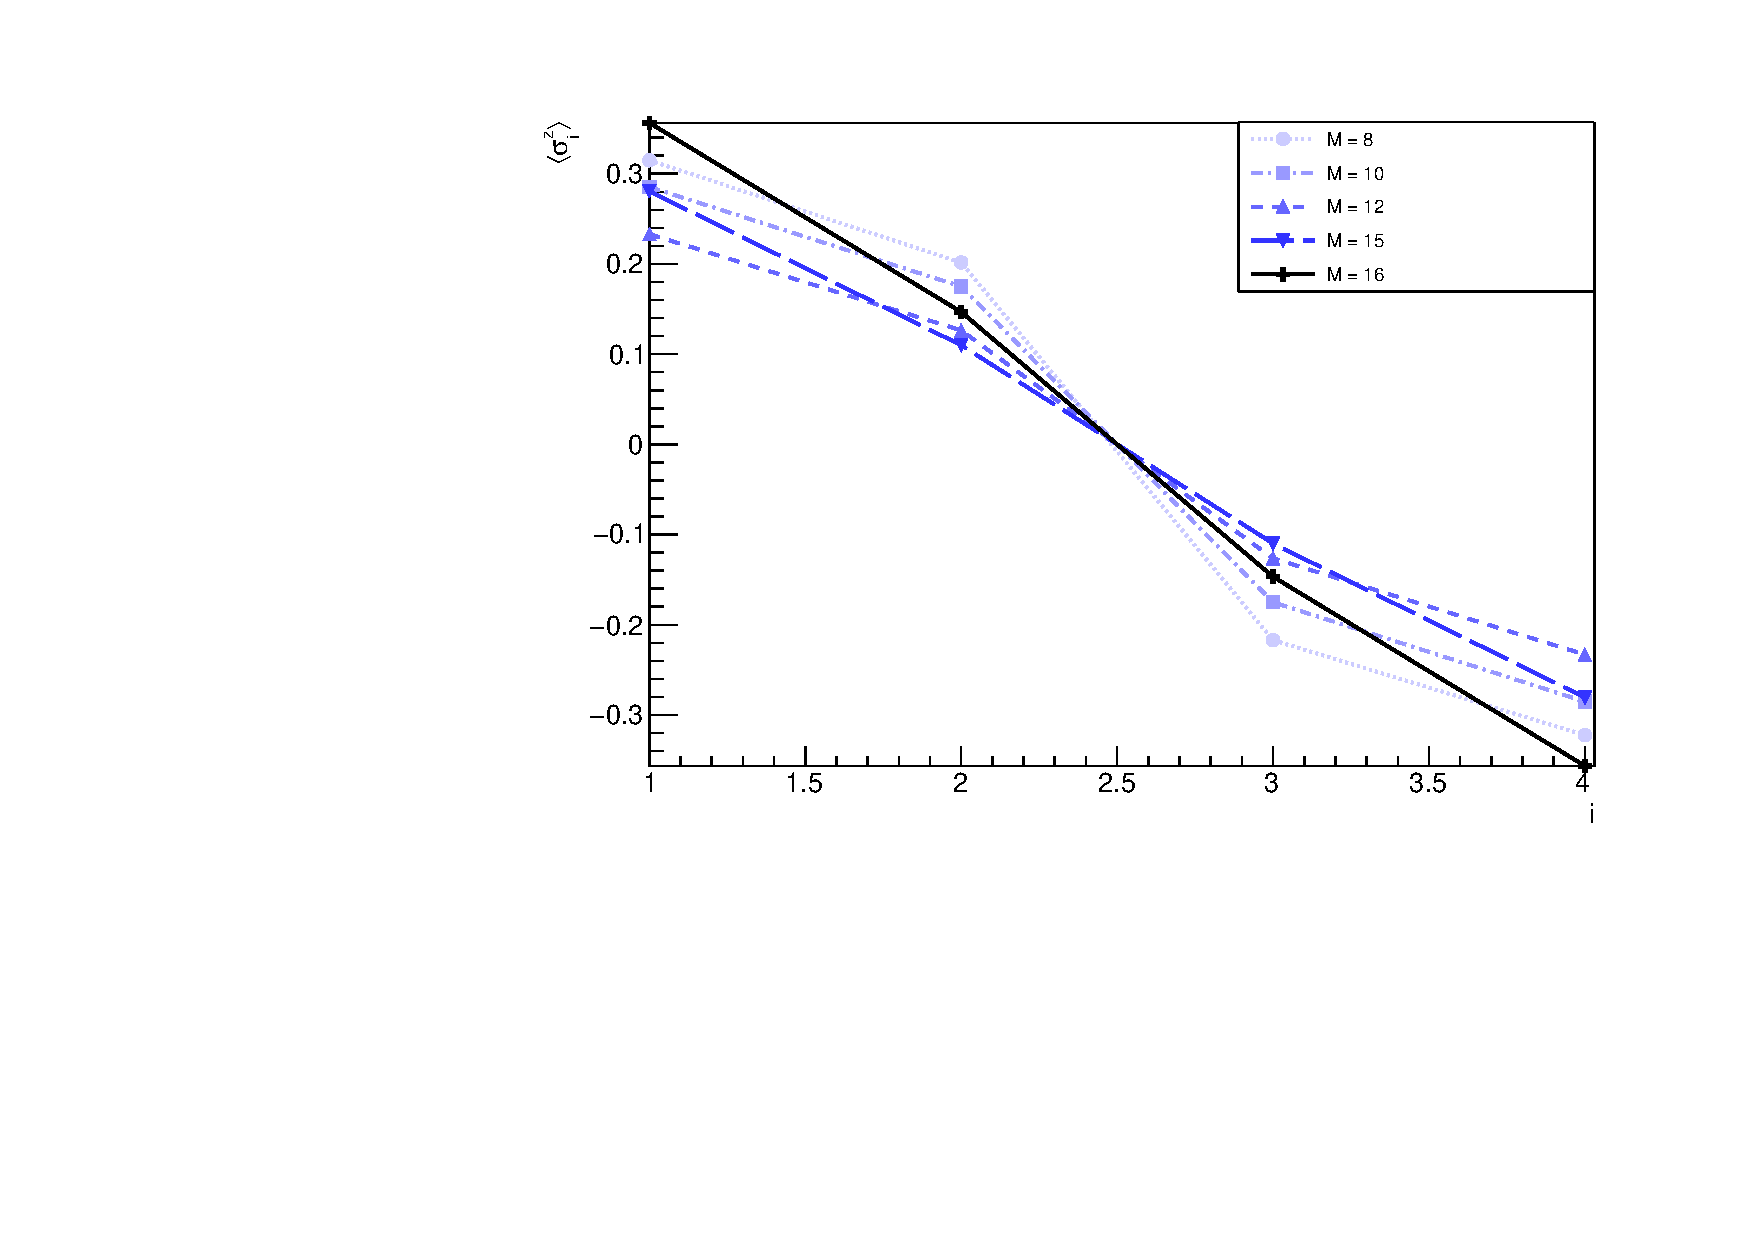
\includegraphics[scale=0.7]{Figures/4sites/4sites_LM_convergenceIncreasingM.pdf}
    \caption{Spin profile of a 4-sites chain for the model described above with $J_z=1$ for several values of corner-space dimensions $M \times M$. The cyan markers are those representing the expectation value of the magnetization calculated by means of a complete set of states of Hilbert space (which has dimension $2^4$).}
    \label{fig:4sites_LM_convergenceIncreasingM}
\end{figure}

As shown in figure~\ref{fig:4sites_LM_convergenceIncreasingM}, it is clear that for such a system the convergence has not been reached. Even for $M = 15$, that covers almost the total Hilbert space dimension, the results are not the convergent ones.

On the other hand, if we consider a model in which every site is coupled to a dissipator, we can see how the magnetization profile gets to convergence starting from $M = 9$ already.


\begin{figure}[H]
    \centering
    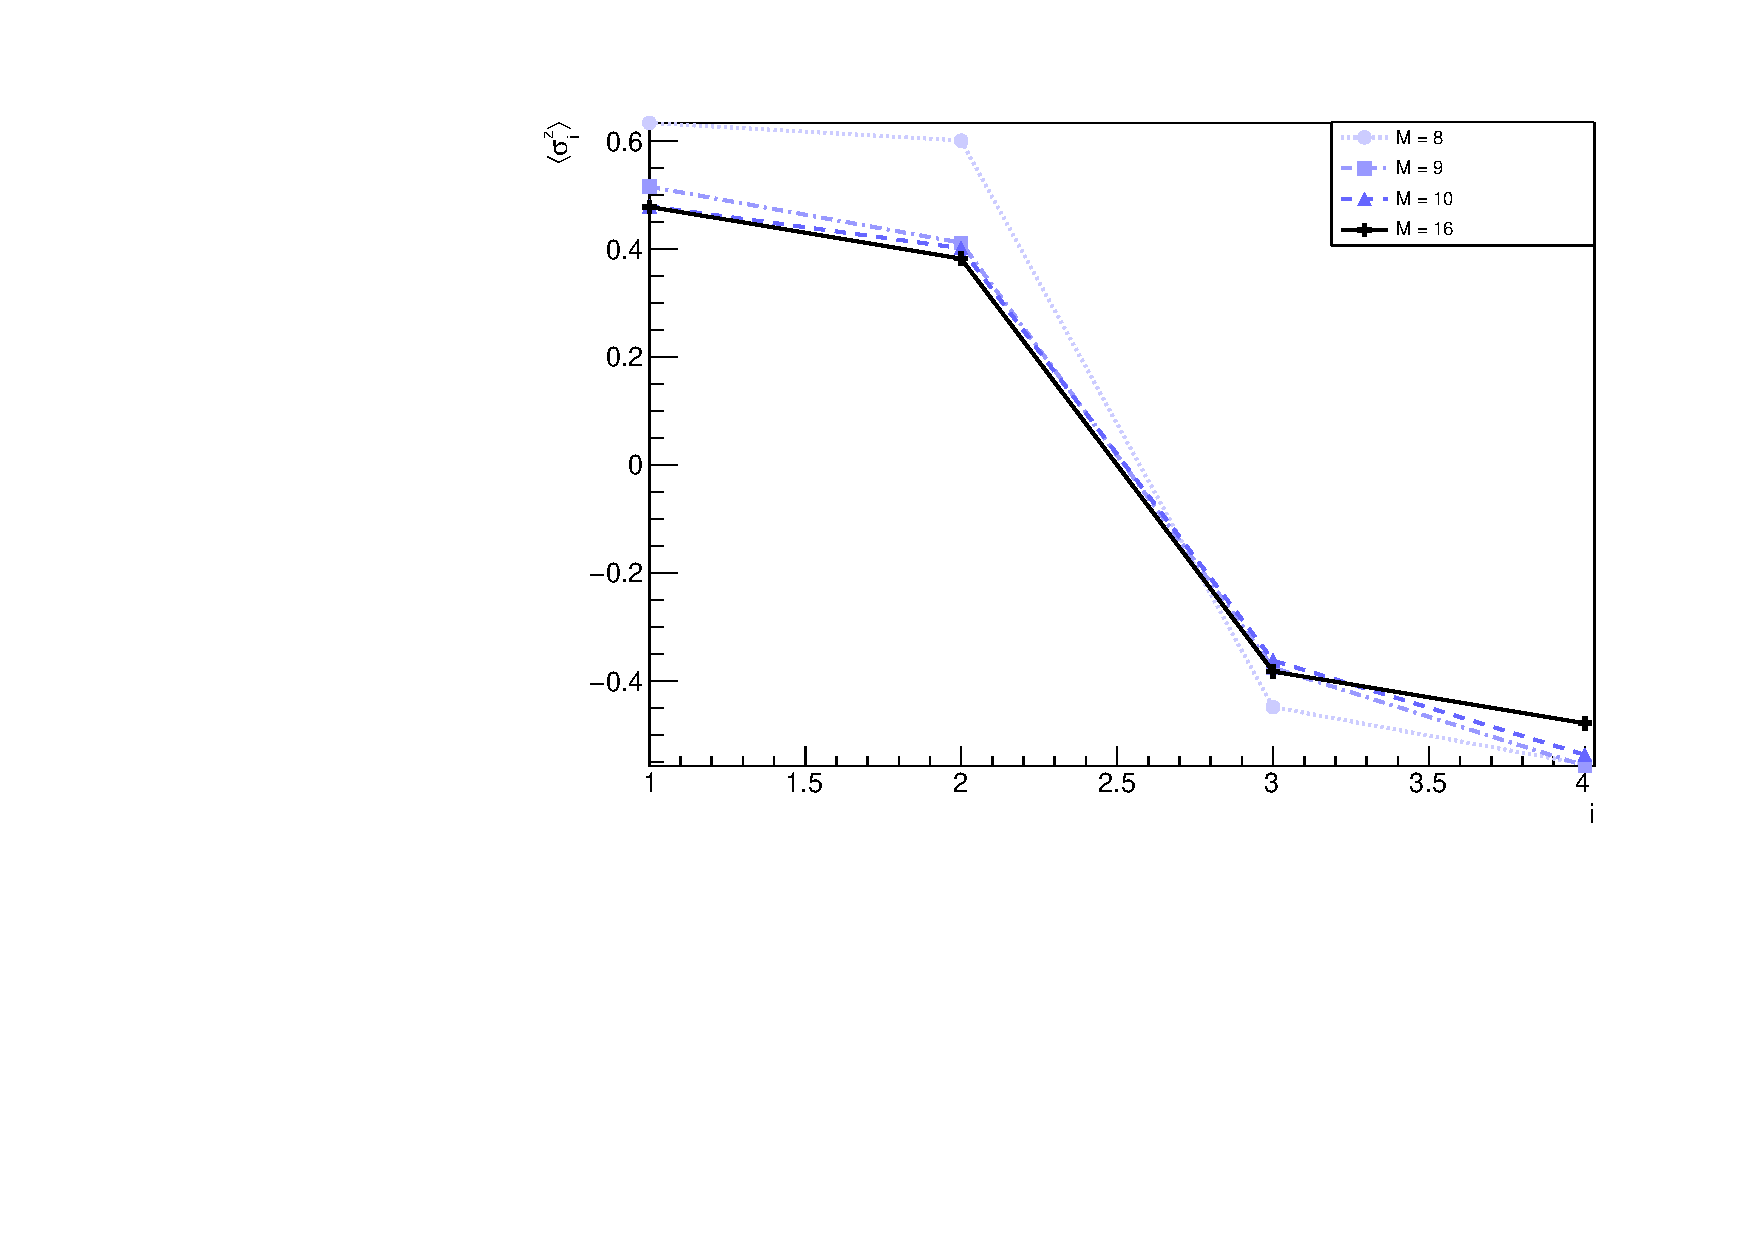
\includegraphics[scale=0.7]{Figures/4sites/4sites_totalDissipators.pdf}
    \caption{Spin profile of a 4-sites chain in which every spin of the chain is coupled to a dissipator. In this case, the convergence is reached for $M<\text{dim}(\mathcal{H})$.}
    \label{fig:4sites_totalDissipators}
\end{figure}

In order to confirm the limitations of this method, the same comparison is done for a longer chain, made up by 8 sites. In this case, the results of CSR method are compared to those of MPO method, since a brute-force diagonalization of the Liouvillian operator would not be possible: it would require a huge amount of memory. We have reason to believe that the results obtained from MPO method are plausible, as we will see in the next sections.

\begin{figure}[H]
    \centering
    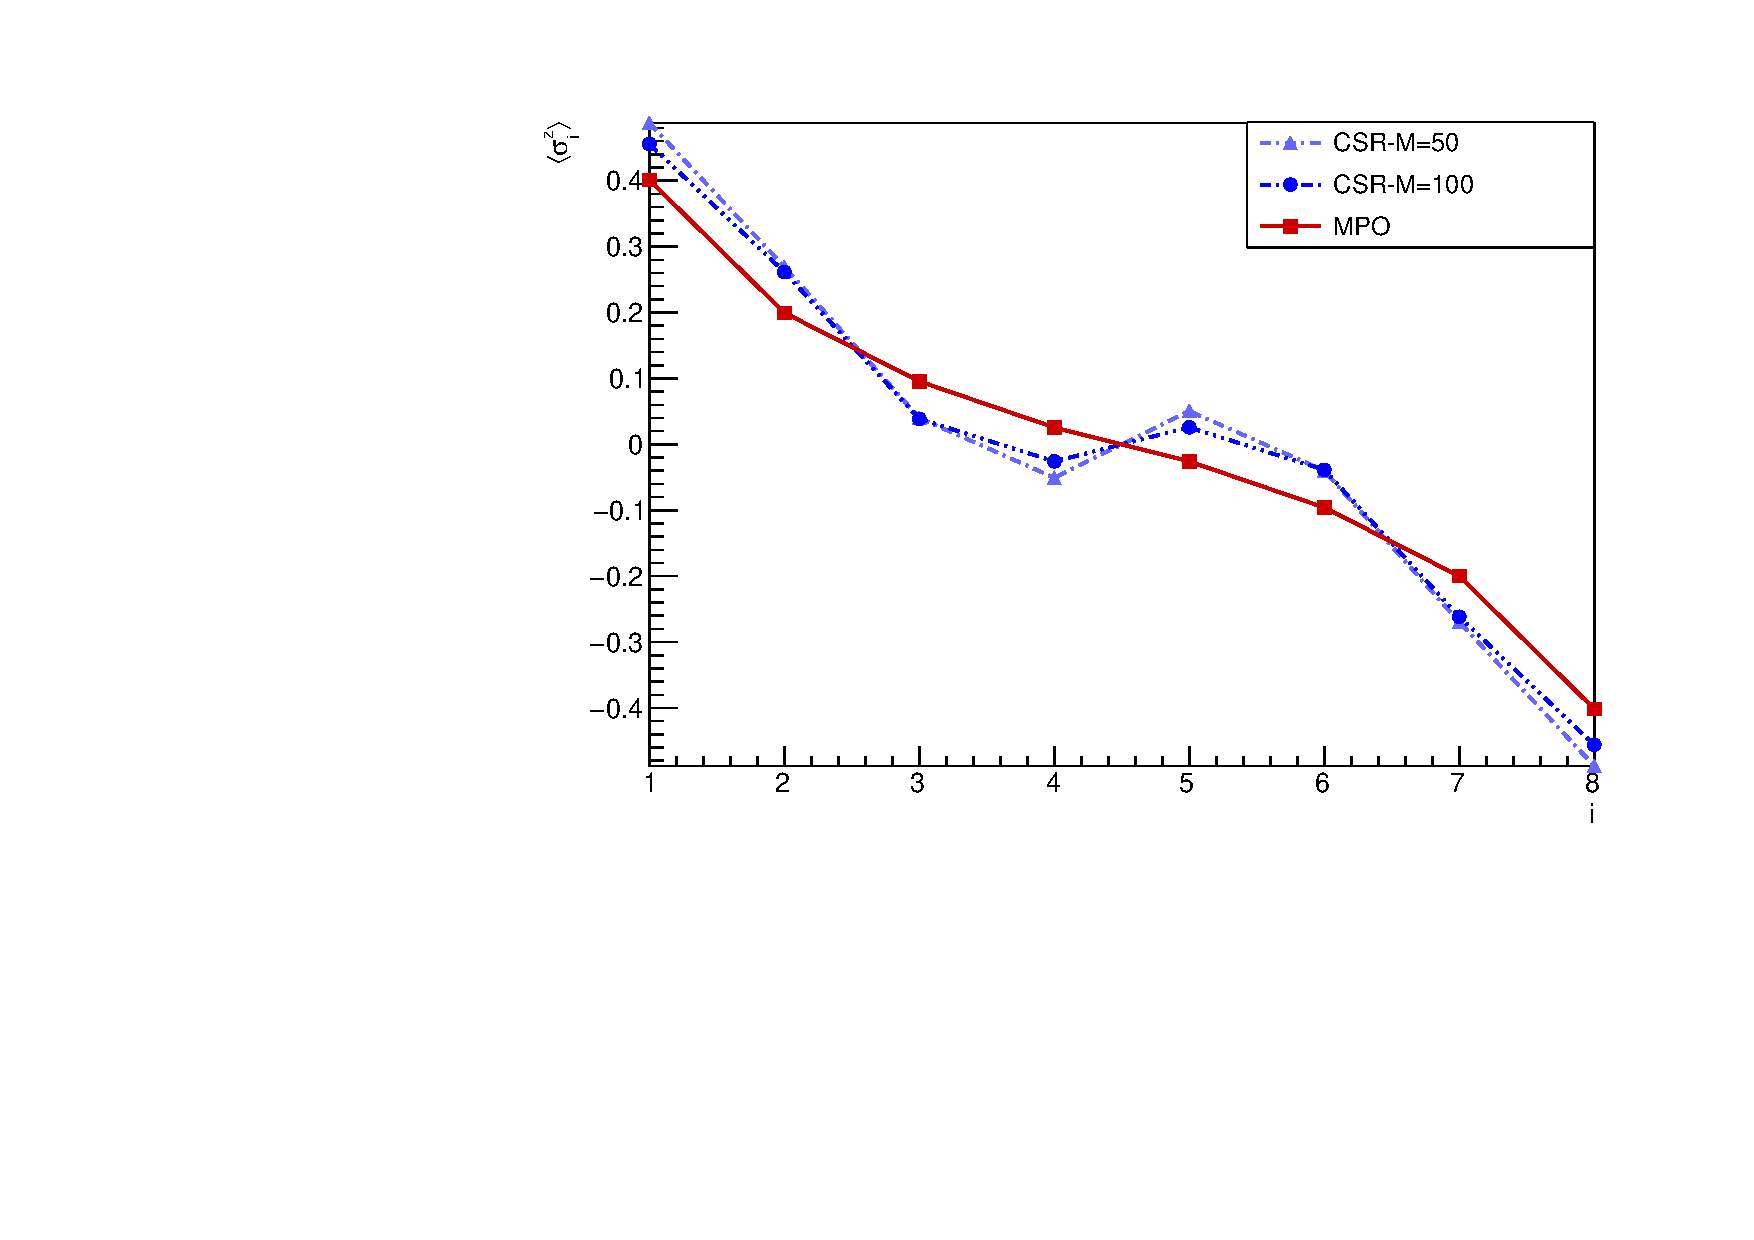
\includegraphics[scale=0.7]{Figures/8sites/1U1D_comparisonCSR_MPO_8site.pdf}
    \caption{Spin profile of a 8-sites chain for the model described in sec.\ref{sec:model}. Significant differences between the data obtained for $M=50$ and $M=100$ are not noticed.}
    \label{fig:1U1D_comparisonCSR_MPO_8site}
\end{figure}

\begin{figure}[H]
    \centering
    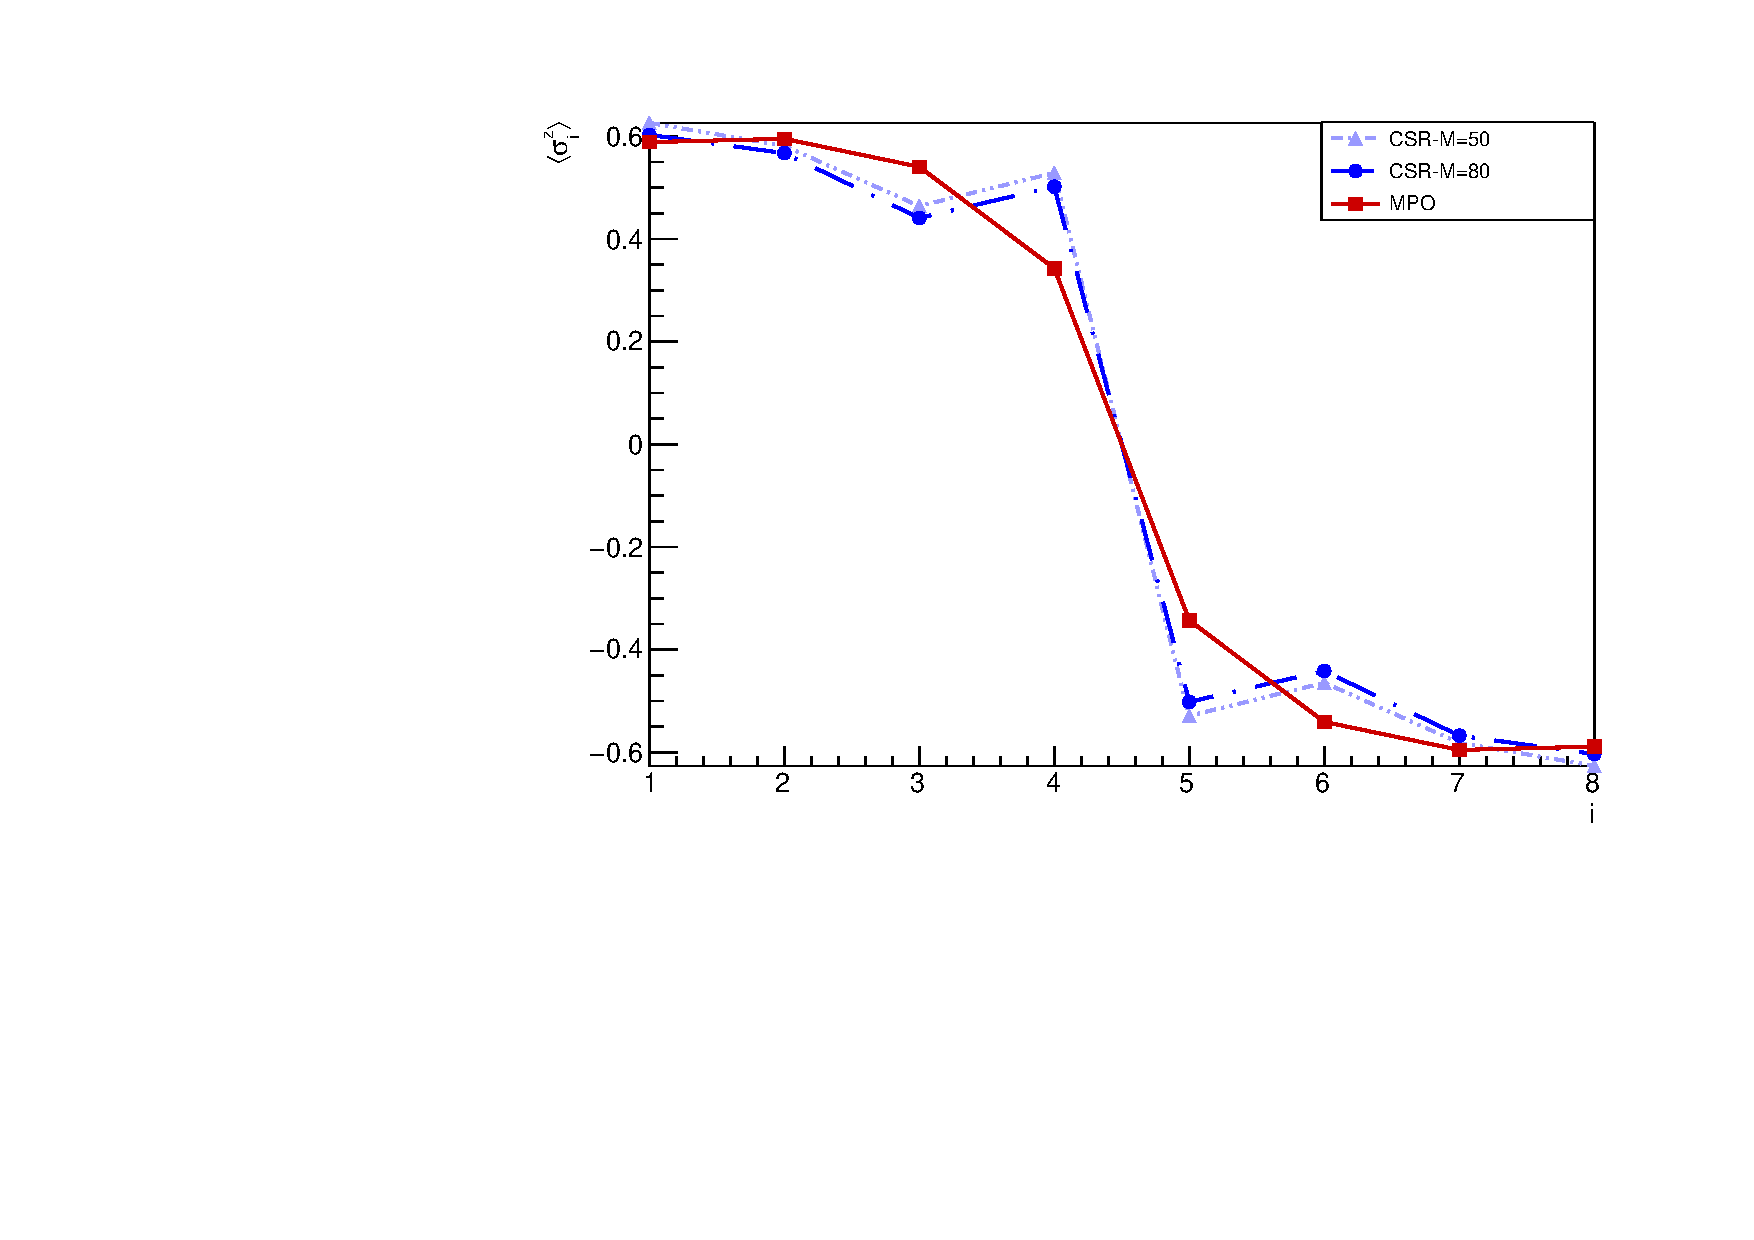
\includegraphics[scale=0.7]{Figures/8sites/8sites_MPOvsCORNER_4U4D.pdf}
    \caption{Spin profile of a 8-sites chain in which every spin of the chain is coupled to a dissipator.}
    \label{fig:8sites_MPOvsCORNER_4U4D}
\end{figure}

In conclusion, in fig.~\ref{fig:LMComparison16s1051} it is displayed the magnetization profile of a 16-sites chain obtained by CSR and MPO methods.

\begin{figure}[H]
    \centering
    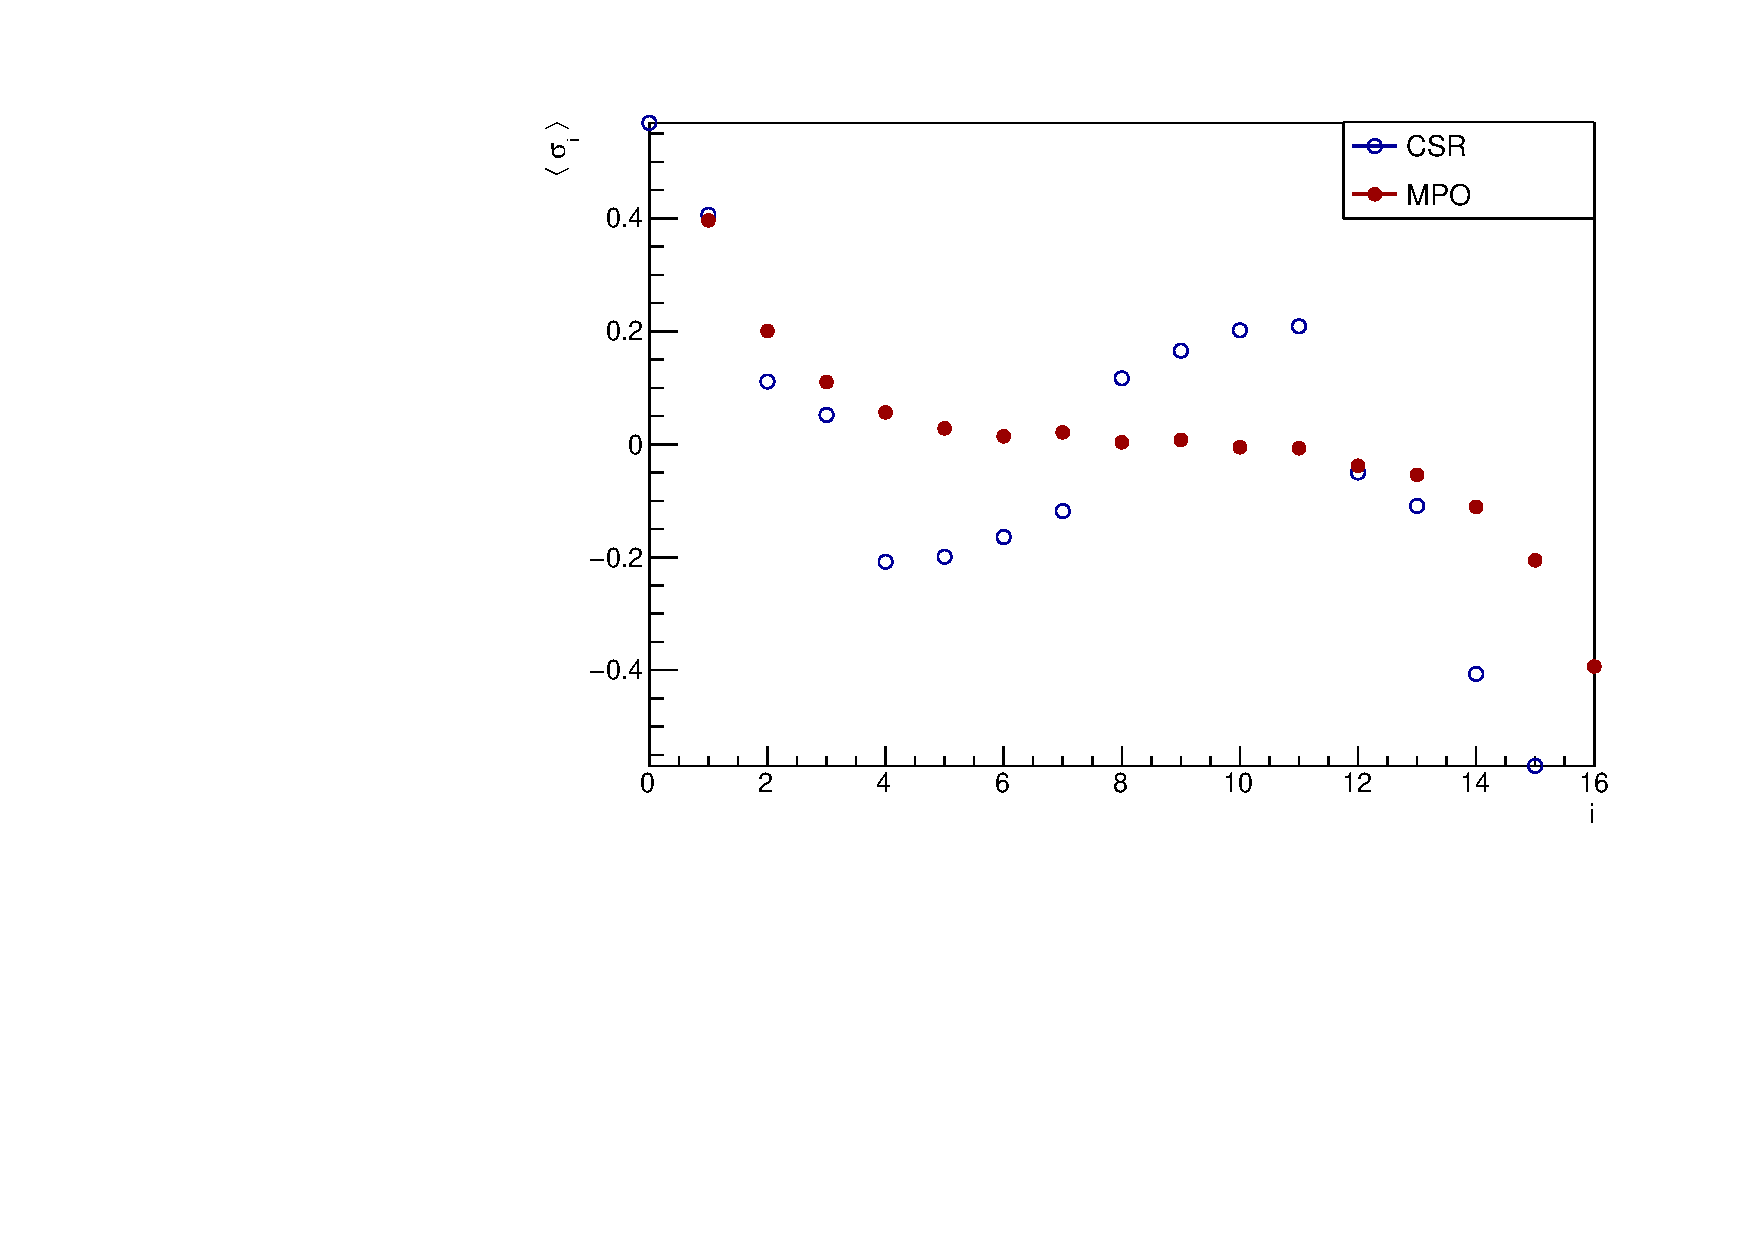
\includegraphics[scale=0.7]{Figures/16sites/LMComparison16s1051.pdf}
    \caption{Spin profile for a 16-sites chain for the model described in section~\ref{sec:model}. Data in red are obtained from MPO method, with m = 80 and T = 2000 and data in blue are obtained from CSR method, with M = 65. It is self-evident the inadequacy of the corner-space method, for the model under study.}
    \label{fig:LMComparison16s1051}
\end{figure}

\begin{figure}[H]
    \centering
    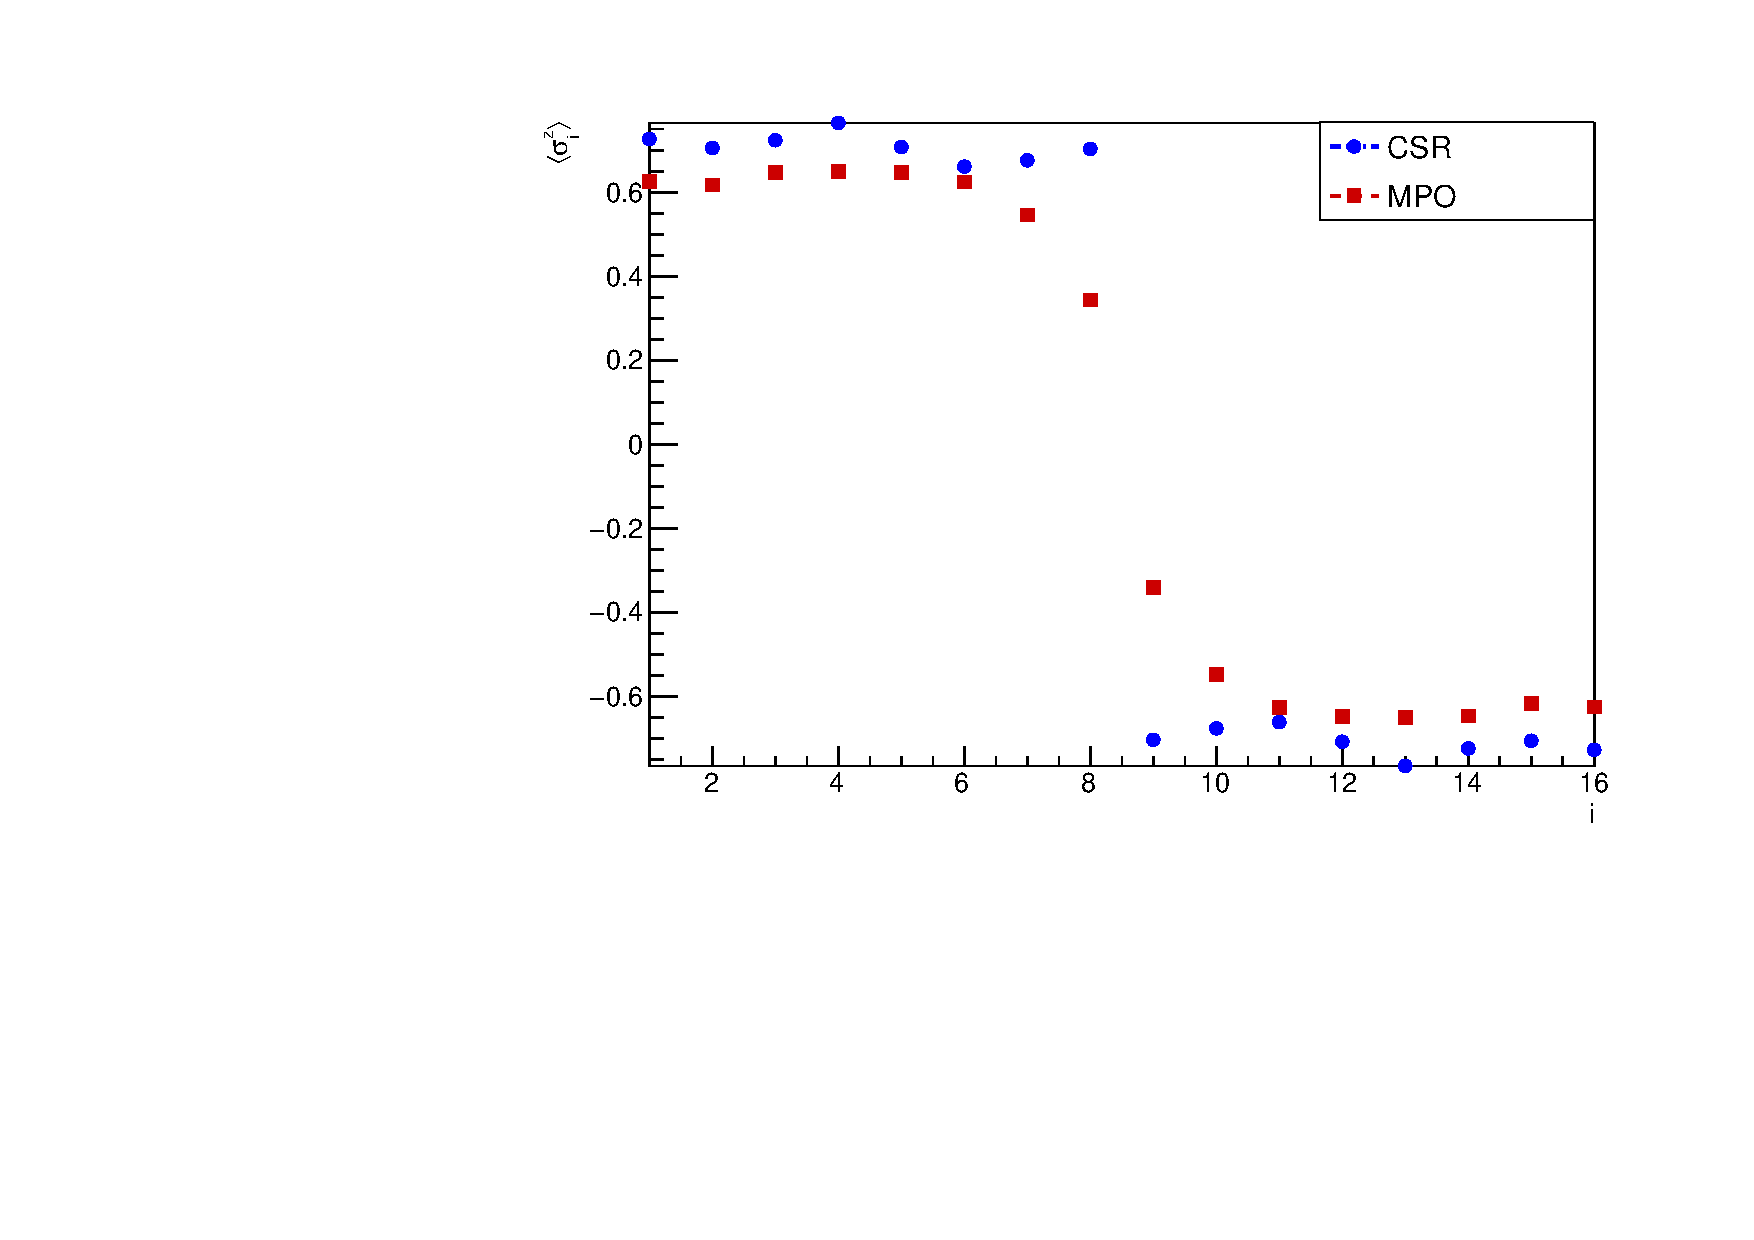
\includegraphics[scale=0.7]{Figures/8U8D_comparisonCSRvsMPO.pdf}
    \caption{Spin profile for a 16-sites chain in which every spin of the chain is coupled to a dissipator. The dimension of the corner-space is $M=65$.}
    \label{fig:LMComparison16s1051}
\end{figure}